% -*-memoria.tex-*-
% Este fichero es parte de la plantilla LaTeX para
% la realización de Proyectos Final de Carrera, protegido
% bajo los términos de la licencia GFDL.
% Para más información, la licencia completa viene incluida en el
% fichero fdl-1.3.tex

% Copyright (C) 2009 Pablo Recio Quijano 

%-------------------------------------------------------
% ---- Plantilla para libros / memorias PFC -----

% Realizada por Pablo Recio Quijano y Noelia Sales Montes 
% Formato de portada y primera página tomado del PFC de
% Francisco Javier Vázquez Púa, en su proyecto 'libgann'
% -------------------------------------------------------

\documentclass[a4paper,11pt]{book}

\usepackage{./estilos/estiloBase} % Basicamente son todas las
                                  % librerias usadas. En caso de que
                                  % falten librerias se van añadiendo
                                  % al fichero.
\usepackage{./estilos/colores}  % Algunos colores ya generados, para
                                % los algunos estilos más avanzados.
\usepackage{./estilos/comandos} % Algunos comandos personalizados

\graphicspath{{./imagenes/}} % Indicamos la ruta donde se encuentran
                             % las imagenes, para ahorrarnos la ruta
                             % completa, y solo modificar aquí si en
                             % un momento dado lo movemos

\begin{document}

% Renombramos las figuras y las tablas
\renewcommand{\figurename}{Figura}
\renewcommand{\listfigurename}{Índice de figuras}
\renewcommand{\tablename}{Tabla}
\renewcommand{\listtablename}{Índice de tablas}
\renewcommand{\lstlistingname}{Listado}
\renewcommand*\lstlistlistingname{Índice de listados}

\pagestyle{empty}
% -*-portada.tex-*-
% Este fichero es parte de la plantilla LaTeX para
% la realización de Proyectos Final de Carrera, protejido
% bajo los términos de la licencia GFDL.
% Para más información, la licencia completa viene incluida en el
% fichero fdl-1.3.tex

% Fuente tomada del PFC 'libgann' de Javier Vázquez Púa

\begin{titlepage}

  \begin{center}

    
\includegraphics[scale=0.2]{logo_uca.png} \\
    
    \vspace{2.0cm}
    
    \LARGE{\textbf{ESCUELA SUPERIOR DE INGENIERÍA}} \\
    
    \vspace{1.0cm}
    
    \Large{\textbf{INGENIERÍA TÉCNICA EN INFORMÁTICA DE GESTIÓN}} \\
    
    \vspace{3.0cm}
    
    \Large{Dominous: simulador libre de dominó} \\
    
    \vspace{2.0cm}
    
    \Large{Ignacio Palomo Duarte} \\
  
    \vspace{0.5cm}

    \large{\today}
    
  \end{center}
\end{titlepage}

\cleardoublepage

% -*-primerahoja.tex-*-
% Este fichero es parte de la plantilla LaTeX para
% la realización de Proyectos Final de Carrera, protejido
% bajo los términos de la licencia GFDL.
% Para más información, la licencia completa viene incluida en el
% fichero fdl-1.3.tex

% Fuente tomada del PFC 'libgann' de Javier Vázquez Púa

\begin{center}

  
\includegraphics[scale=0.2]{logo_uca.png} \\

  \vspace{2.0cm}

  \Large{ESCUELA SUPERIOR DE INGENIERÍA} \\

  \vspace{1.0cm}

  \large{INGENIERO TÉCNICO EN INFORMÁTICA DE GESTIÓN} \\

  \vspace{2.0cm}

  \large{DOMINOUS: SIMULADOR LIBRE DE DOMINÓ} \\

  \vspace{1.0cm}

\end{center}

\begin{itemize}
\item \large{Departamento: Lenguajes y Sistemas Informáticos}
\item \large{Directores del proyecto: Manuel Palomo Duarte e Inmaculada Medina Bulo}
\item \large{Autor del proyecto: Ignacio Palomo Duarte}
\end{itemize}

\vspace{1.0cm}

\begin{flushright}
  \large{Cádiz, \today} \\

  \vspace{2.5cm}

  \large{Fdo: Ignacio Palomo Duarte}
\end{flushright}

\cleardoublepage
\pagestyle{plain}

\frontmatter % Introducción, índices ...

% -*-previo.tex-*-
% Este fichero es parte de la plantilla LaTeX para
% la realización de Proyectos Final de Carrera, protegido
% bajo los términos de la licencia GFDL.
% Para más información, la licencia completa viene incluida en el
% fichero fdl-1.3.tex

% Copyright (C) 2009 Pablo Recio Quijano 

\section*{Agradecimientos}

Gracias a los que han estado conmigo desde siempre, a las nuevas incorporaciones y, sobre todo, a mi padre.

\cleardoublepage

\section*{Licencia} % Por ejemplo GFDL, aunque puede ser cualquiera

Este documento ha sido liberado bajo Licencia GFDL 1.3 (GNU Free
Documentation License). Se incluyen los términos de la licencia en
inglés al final del mismo.\\

Copyright (c) 2011 Ignacio Palomo Duarte.\\

Permission is granted to copy, distribute and/or modify this document under the
terms of the GNU Free Documentation License, Version 1.3 or any later version
published by the Free Software Foundation; with no Invariant Sections, no
Front-Cover Texts, and no Back-Cover Texts. A copy of the license is included in
the section entitled "GNU Free Documentation License".\\

\cleardoublepage

\section*{Notación y formato}

Cuando nos refiramos a un programa en concreto, utilizaremos la
notación: \programa{emacs}.\\

Cuando nos refiramos a un comando, o función de un lenguaje, usaremos
la notación: \comando{quicksort}.\\

Extractos de ficheros con texto plano o código aparecerán

\begin{lstlisting} [language=Python, numbers=left]
class nombre_de_la_regla:
    def __init__(self):
        # inicializamos los atributos que sean necesarios
        pass
    def go(self, left_tile, right_tile, board, tiles, log):
        return ficha, lado, tiempo_pensando
\end{lstlisting}

\cleardoublepage

\tableofcontents
\listoffigures
\listoftables
\lstlistoflistings


\mainmatter % Contenido en si ...

\chapter{Introducción}
% -*-cap1.tex-*-
% Este fichero es parte de la plantilla LaTeX para
% la realización de Proyectos Final de Carrera, protejido
% bajo los términos de la licencia GFDL.
% Para más información, la licencia completa viene incluida en el
% fichero fdl-1.3.tex

% Copyright (C) 2009 Pablo Recio Quijano 

\section{¿Por qué un simulador de dominó}

A la hora de embarcarse en el desarrollo de un Proyecto Fin de Carrera, la primera duda es obvia: ¿Sobre qué va a versar mi proyecto?.

El Proyecto Fin de Carrera es el culmen a un largo período de aprendizaje, exámenes y vivencias y experiencias, y por estas razones la elección de una temática para el proyecto es compleja, ya que tenemos diferentes necesidades, limitaciones e impulsos:
\begin{enumerate}
    \item Por una parte el proyecto es una facción más de nuestros estudios universitarios, que debemos solventar con éxito, y esta circunstancia nos puede llevar a buscar un proyecto más recortado o limitado en cuanto a requerimientos de tiempo y conocimiento.
    \item Pero por otra parte nuestra faceta de ingenieros nos impulsa a aprender, a enfrentarnos con nuevos problemas y dificultades, a atacar ejercicios mentales duros e interesantes para hacer sudar nuestra mente.
\end{enumerate}

Y después de tantear varios proyectos que tenía en mente, mi tutor me presentó la posibilidad de embarcarme en el desarrollo de un simulador de dominó. Al principio tomé la idea un poco en broma, ya que la temática en principio puede parecer poco tecnológica, demasiado localizada o con escaso atractivo, pero una vez analizado, el proyecto tenía todo lo que le podía pedir:
\begin{enumerate}
    \item El apartado de Inteligencia Artificial es muy complejo, con lo cual se puede abordar de diferentes maneras, aplicando diferentes técnicas de sistemas expertos. Además es un problema de elevada complejidad computacional si intentamos resolverlo mediante simples árboles de decisión: como el juego se desarrolla dentro de un marco de conocimiento limitado (no conocemos las fichas de los demás jugadores) se produce una explosión combinatoria que nos obliga a buscar otros métodos y herramientas.
    \item Por otro lado FIXME
\end{enumerate}

\section{Estructura de la memoria}


\chapter{Conceptos básicos}
% -*-cap2.tex-*-
% Este fichero es parte de la plantilla LaTeX para
% la realización de Proyectos Final de Carrera, protegido
% bajo los términos de la licencia GFDL.
% Para más información, la licencia completa viene incluida en el
% fichero fdl-1.3.tex

% Copyright (C) 2009 Pablo Recio Quijano 

En este capítulo se comentarán las bases del proyecto: fundamentos del dominó y diseño de sistemas expertos.

\section{El dominó}

A continuación se detalla una breve historia del juego del dominó y similares y después se comentan las estrategias fundamentales para jugar el dominó internacional (el que normalmente suele jugarse en España e Iberoamérica).

\subsection{Historia del dominó}

El dominó, deporte y pasatiempo a un tiempo, es un juego que ha ganado adeptos a lo largo de la historia. Según explica \textbf{Miguel Lugo} en su libro Dominó Competitivo \cite{lugo08} éste “es entretenido y fácil de
aprender. Ya desde pequeños comenzamos a jugar al dominó con frutas o con animales en lugar de hacerlo
con puntos”. Además, éste ha ganado popularidad durante los últimos años hasta el punto de televisar
torneos en Europa, Norteamérica y Latinoamérica.

\begin{quote}
“En 2001 la Federación Internacional de Dominó (con sede en Barcelona, España) celebró el primer
Congreso Internacional. El año siguiente se llevó a cabo el primer Campeonato del Mundo de Dominó en La
Habana (Cuba). El ‘Mundial’ continúa celebrándose anualmente a partir de este punto, en España, México,
Venezuela y EEUU" (Lugo, 2008: 1).
\end{quote}

Así pues Lugo señala que el dominó nunca antes ha estado tan reconocido en todo el mundo como ahora, que
incluso se puede jugar por Internet. \\

La página web Dominó en Línea \cite{website:dominoenlinea} recoge que en la actualidad el dominó se juegan en todo el
mundo aunque resalta que es “especialmente popular en América Latina, donde los dominós se consideran
como el juego nacional de numerosos países del Caribe”. Así, también menciona los torneos anuales y
los clubes locales de dominó.

\begin{quote}
El origen del dominó parece ser muy antiguo, al menos en lo que se refiere a juegos similares y quizá
pretéritos al actual” (González Sanz, 2010:22)
\end{quote}

Cuenta \textbf{González Sanz} en su libro El arte del dominó: teoría y práctica \cite{sanz00} que algunos historiadores
creen que puede tener origen chino, ya que éstos jugaban a un juego parecido con impresiones en piedra. Este pudo llegar a Europa a través de mercaderes y viajeros, entre los que se cita al célebre
Marco Polo, los cuales y fruto de los intercambios culturales de la época, trajeron el dominó a este
lado del mundo, más en concreto a la Península Itálica, primer lugar de Europa donde se ha datado la
práctica de este juego. \\

\textbf{Benito Ruipérez} \cite{mora90} también señala que se trata de un juego muy antiguo, de unos 400 años de historia,
aunque dice que se desconoce su origen y etimología (1990:7). Por otro lado, este autor comenta que
llego a Italia desde China en el siglo XVIII, sin embargo, relata que no está probado. “Versiones
coincidentes aseguran que el dominó entró en Europa a través de Italia (con lo que también se puede
atribuir su invención a los italianos, al menos el sistema de juego europeo)”, recoge Ruipérez. \\

Los italianos lo pusieron de moda introduciéndolo en España y Francia a mediados del siglo XVIII,
llegando más tarde a popularizarse de modo extraordinario. A finales del mismo siglo apareció en
Inglaterra, donde fue calificado de ‘juego infantil’, según Ruipérez “nada más lejos de la realidad”.
\textbf{Joseph Strutt} publicó un libro Deportes y Pasatiempos en 1801, en el que, entre otros disparates,
demostró un gran desconocimiento del juego. Así, escribió: “El dominó no tiene mayor interés que
el ponerlo en conocimiento de las personas mayores de este país” (Ruipérez, 1990:7). \\

Precisamente \textbf{Martin Gardner}, experto en juegos, explica que en la literatura occidental no hay
referencias a este juego hasta mediados del siglo XVIII, en que empezaron a jugarse en Italia y
Francia las primeras partidas. Desde ahí, el juego se extendió al resto del continente, y más tarde,
a Inglaterra y América. En Occidente, la colección normal de piezas de dominó ha consistido siempre
en 28 teselas o losetas formadas por dos cuadrados adyacentes, que contienen todos los posibles
pares de dígitos, de 0 hasta 6. \\

\begin{figure}[h]
  \label{Martin_Gardner}
  \begin{center}
    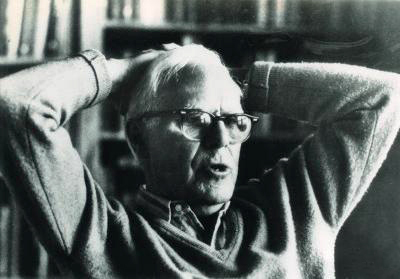
\includegraphics[scale=0.5]{Martin_Gardner.jpeg}
  \end{center}
  \caption{Martin Gardner, divulgador científico y filósofo de la ciencia estadounidense.}
\end{figure}


Respecto al juego chino, Gardner, que colaboró más de 20 años en la sección “Juegos Matemáticos” de
la revista \textbf{Scientific American}, comenta en su libro Circo Matemático que en los dominós chinos,
llamado kwat p’ai, no existen piezas con caras en blanco. Éstos contienen todas las combinaciones
por pares desde el (1-1)  hasta el (6-6), donde tres de los seis puntos de cara son también rojos.
Los dominós coreanos son idénticos, con la única particularidad de que en el as, el punto es mayor
que en las demás piezas. En los dominós chinos, cada pieza tiene un nombre pintoresco: el (6-6)
es el “cielo”; el (1-1) es “la tierra”, el (5-5) es la “flor del ciruelo”, el (6-5), “la cabeza de
tigre”, etc. Los nombres de las piezas son iguales a los que reciben los 21 resultados posibles del
lanzamiento de un par de dados. \\

Ruipérez añade que el invento se les achaca a los chinos “pero no ha de ser muy fiable, ya que el
dominó de chinos y coreanos es muy distinto al que se practica en Europa” (1990:7). Así lo describe
en su Libro del dominó:

\begin{quote}
“El dominó oriental consta de 21 fichas, que representan las permutaciones matemáticas resultantes
de tirar dos dados (cada mitad de una ficha vale por un lado), el ‘uno’ y el ‘cuatro’ son rojos;
además, en los dados chinos intervienen 11 fichas repetidas, con lo que suman un total de 32 fichas
el conjunto de, y para, este juego. Las fichas repetidas se llaman ‘civiles’ y las otras ‘militares’,
distinción importante para ciertos juegos de dominó en China y Corea”.
\end{quote}

González Sanz (2010:22) señala que los dominós chinos “suelen ser en la actualidad de cartón, en vez
de la madera, marfil, pasta, o ébano que es lo habitual en los occidentales, y se manejan como naipes”.
Y al igual que ocurre en Europa y América, con estas piezas se realizan numerosos juegos. Respecto a
los distintos juegos de dominó chinos y coreanos, este autor nos remite a Games of the Orient de Stewart
Culin, obra de 1895 reimpresa en 1958 por Charles Tuttle como la mejor referencia. Asimismo apunta que
no existe un dominó propio en Japón – frente al resto de países asiáticos – y dice que en este país se
juega con el sistema occidental. \\

\begin{figure}[h]
  \label{}
  \begin{center}
    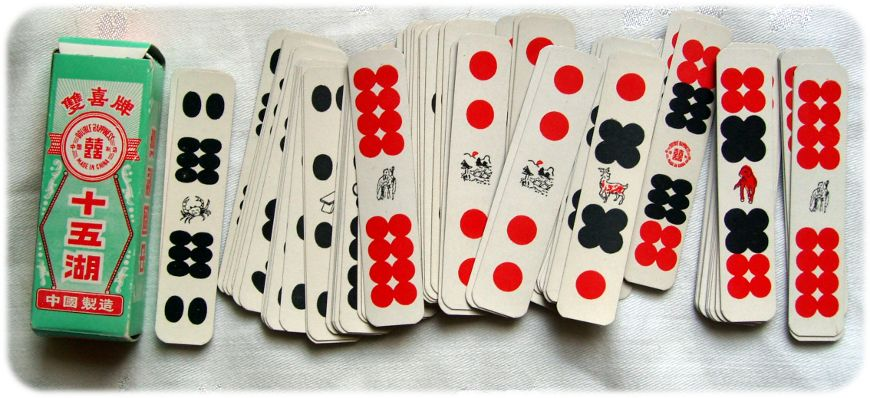
\includegraphics[scale=0.6]{chinese.jpg}
  \end{center}
  \caption{Cartas de dominó chino \textbf{“Double Happiness”} --- los símbolos representan diferentes
            circunstancias y bendiciones de la vida }
\end{figure}

Sin embargo, y aunque por lo que señalan algunos autores el origen asiático del dominó es el más
extendido, también existen otras versiones que atribuyen el invento del juego a árabes o egipcios,
“sosteniendo que no hay pruebas para relacionar claramente el dominó europeo con el chino, pudiendo
ser dos invenciones independientes y separadas en el tiempo” (2010:23). González también cuenta que
se conocen otras versiones del juego como la esquimal o la coreana, con distinto número de fichas
y palos al clásico. \\

Por otro lado, otros autores (desde la página Dominó en Línea \cite{website:dominoenlinea}) apuntan que el dominó
de origen más antiguo se habría encontrado en la tumba de Touthankamon en Egipto. Y que los dominós nacieron de la derivación del juego de dados indio, conocido en Europa bajo el dado a seis-cara, los chinos modificaron este dado en parte plana reversible representando puntos, de 1 en 6 puntos. En Europa sería apareció una cara suplementaria, el blanco. \\

En el apartado de curiosidades que se apunta en esta web podemos destacar que la palabra “dominó”
sería a causa de la semejanza entre las partes de las fichas del juego y la ropa de las religiosas
de las Dominicas (blanco cubierto de un cabo negro). Sin embargo, el autor Ruipérez en el Libro
del Dominó apunta otros posibles orígenes al término, algunos muy parecidos al ya apuntado. De hecho, existe una variante del juego que se juega con fichas de tres caras y se llama \emph{Trimino}, haciendo un juego de do(s)-mino por tri-mino \cite{website:trimino}\\

En este sentido, señala este autor que su nombre se debe, según unos, al revestimiento negro que
llevan sus fichas por el reverso (la espalda), como si fueran cubiertas por un dominó (capuchón
que usaban en el coro, durante el invierno, los monjes). Y según otros, a que tal juego, por su
sencillez, “prueba inequívoca de que no se conocían las técnicas que se usan hoy en día, o de alta
escuela, que son las que se explican en este libro”, estuvo muy en uso en los conventos, y cuando
uno de los jugadores ganaba una partida decía: ‘Benedicamus Dómino’. Una tercera versión para
explicar el nombre afirma que por aquel entonces alguien ya detectó que para ‘manejar’ bien estas
fichas tenía que tener ‘dominio’ de sí mismo (control de lo jugado y de lo pendiente por jugar) en
cada mano, y podría decir, cada vez que querían jugar con estas fichas, ‘vamos a practicar unas
manos al juego del dominio’, habiendo degenerado o perfeccionado el dicho hasta quedar en el juego
del dominó (Ruipérez, 1990:9). \\

En cuanto a la documentación escrita de este juego, este mismo autor,
Ruipérez, señala que el primer libro que hace referencia al juego del
dominó data del año 1786, editado en Amsterdam, según consta en la
Biblioteca Nacional de Bruselas. En total, este autor señala que hay
más de un centenar de libros hasta la fecha (1984), según consta
también en distintas bibliotecas nacionales de Europa y
Latinoamérica. Aunque para este autor no han tenido suficiente éxito
porque no se profundiza en el tema sino que se relatan someramente las
reglas básicas del mismo. En una consulta en la Biblioteca Nacional
aparece como primer libro en español sobre el tema \textbf{Tratado del Juego del Domino, sus Reglas, Combinaciones y Preceptos para ser un buen jugador} de Martínez~\cite{Martinez}, publicado en 1872. \\

En 1982 y después en 1984, más reformado y actualizado, aparece en Barcelona el libro \textbf{ABC del dominó},
de J.M. Vilabella, que denota un conocimiento más amplio del tema comparado con lo que se había
escrito hasta ese momento, dando explicaciones más amplias de cómo se desarrollan las jugadas,
“aunque muy pocas y con muy pocas variantes”, (Ruipérez, 1990:8)

\subsubsection{Tipología de dominós}

Como hemos visto, a lo largo y ancho del mundo existen diferentes tipos de dominó de los que no
siempre los autores coinciden con un solo origen. Aunque para catalogar tales juegos como dominó sí
deben tener una serie de características en común. 

\begin{quote}
Generalizando el concepto de dominó, podríamos decir que es un juego cuyas fichas se encuentran
divididas en dos partes, las cuales señalan mediante incisiones o muescas, un número concreto entre
los posibles palos o números admitidos. Estas fichas contendrán en su totalidad todas las
combinaciones posibles de estos palos, comenzando por la ausencia de puntos o palo de blancos
(González Sanz, 2010:24).
\end{quote}

La Real Academia de la Lengua Española en su primera acepción define este juego como aquel que
“se hace con 28 fichas rectangulares divididas en dos cuadrados, cada uno de los cuales lleva marcados
de uno a seis puntos, o no lleva ninguno. Cada jugador pone por turno una ficha que tenga número
igual en uno de sus cuadrados al de cualquiera de los dos que están en los extremos de la línea de
las ya jugadas, y gana quien primero coloca todas las suyas o quien se quede con menos puntos, si
se cierra el juego”. De este modo, la RAE acota algo más el término acercándose a lo que conocemos
como dominó occidental. \\

\begin{figure}[h]
  \label{Dominoes}
  \begin{center}
    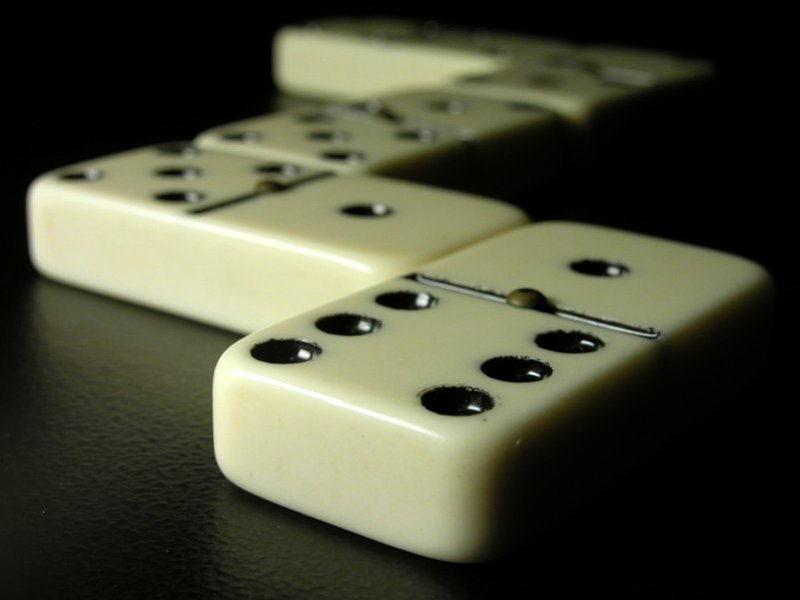
\includegraphics[scale=0.3]{Dominoes.jpg}
  \end{center}
  \caption{Fichas de dominó europeo}
\end{figure}

Según la página Dominó en Línea \cite{website:dominoenlinea} “los dominós son de simples bloques de construcción
que pueden armarse de innombrables maneras con el fin de crear una gran variedad de juegos. Es un
juego que exige mucha capacidad y de estrategia”. \\

Ruipérez define el domino europeo en “un conjunto de veintiocho fichas, por lo general negras y
totalmente lisas por un lado, el reverso o la espalda, y por el otro lado, el anverso o la cara,
divididas en dos mitades con fondo blanco y señaladas con agujeros o puntitos negros; en el centro
de la cara llevan un tornillito con cabeza redondeada, que es el que apoya en la mesa y facilita
el movimiento de las fichas cuando éstas han de ser movidas (barajadas), para que los participantes
cojan sus fichas e inicien la jugada o la mano correspondiente. Tiene siete fichas denominadas
dobles, por en sus medias partes de la cara la misma cantidad de puntitos, a excepción de la
doble blanca, que no lleva ninguno”. \\

\subsection{Reglas básicas}

Aunque las reglas del dominó son sencillas y conocidas por un gran conjunto de lectores, daremos una
serie de pinceladas rápidas sobre las reglas más básicas, siempre recordando que estamos desarrollando
una partida de dominó siguiendo las reglas de la modalidad \emph{Dominó Internacional}. \\

El objetivo del juego es alcanzar una determinada puntuación previamente fijada, jugando para ello las
manos o rondas que sean precisas. En el caso del Dominó Internacional, el número de puntos son 200. En esta modalidad se enfrentan dos equipos, cada uno formado por una pareja de jugadores dispuestos en la mesa de forma alternativa. \\

Antes de empezar, las fichas se colocan boca abajo sobre la mesa y se revuelven para que los jugadores
las recojan al azar en igual número cada uno. Cada jugador cogerá 7 fichas. La primera ronda la comenzará
el jugador que posea el seis doble. En las siguientes rondas, empezará el jugador a la derecha del que
empezó la ronda anterior. Podrá comenzar usando cualquier ficha, no tiene porqué ser doble. \\

En su turno cada jugador colocará una de sus piezas con la restricción de que dos piezas sólo pueden
colocarse juntas cuando los cuadrados adyacentes sean del mismo valor. Si un jugador no puede colocar
ninguna ficha en su turno tendrá que pasar el turno al siguiente jugador. \\

La mano continúa hasta que se da alguna de las dos situaciones:
\begin{itemize}
    \item Alguno de los jugadores se queda sin fichas por colocar en la mesa. En este caso el jugador se
        dice que dominó la partida y la pareja ganadora sumará la totalidad de los puntos no jugados,
        es decir, la suma de los puntos en las fichas que resten por jugar a ambas parejas.
    \item En caso de cierre --- es decir, cuando a pesar de quedar fichas en juego ninguna pueda colocarse ---
        ganará la pareja cuyas fichas sumen menos puntos. Esta situación solamente ocurre cuando el mismo número
        está en ambos extremos del juego, y las siete fichas de ese número ya han sido jugadas. En este caso
        gana la pareja/jugador que menos puntos tenga en sus fichas, y se le suman los puntos del perdedor al ganador.
        Al igual que en el anterior caso, la pareja ganadora sumará la totalidad de los puntos no jugados,
        es decir, la suma de todos los puntos en las fichas que resten por jugar a ambos equipos.
\end{itemize}

\begin{figure}[h]
  \label{cierre}
  \begin{center}
    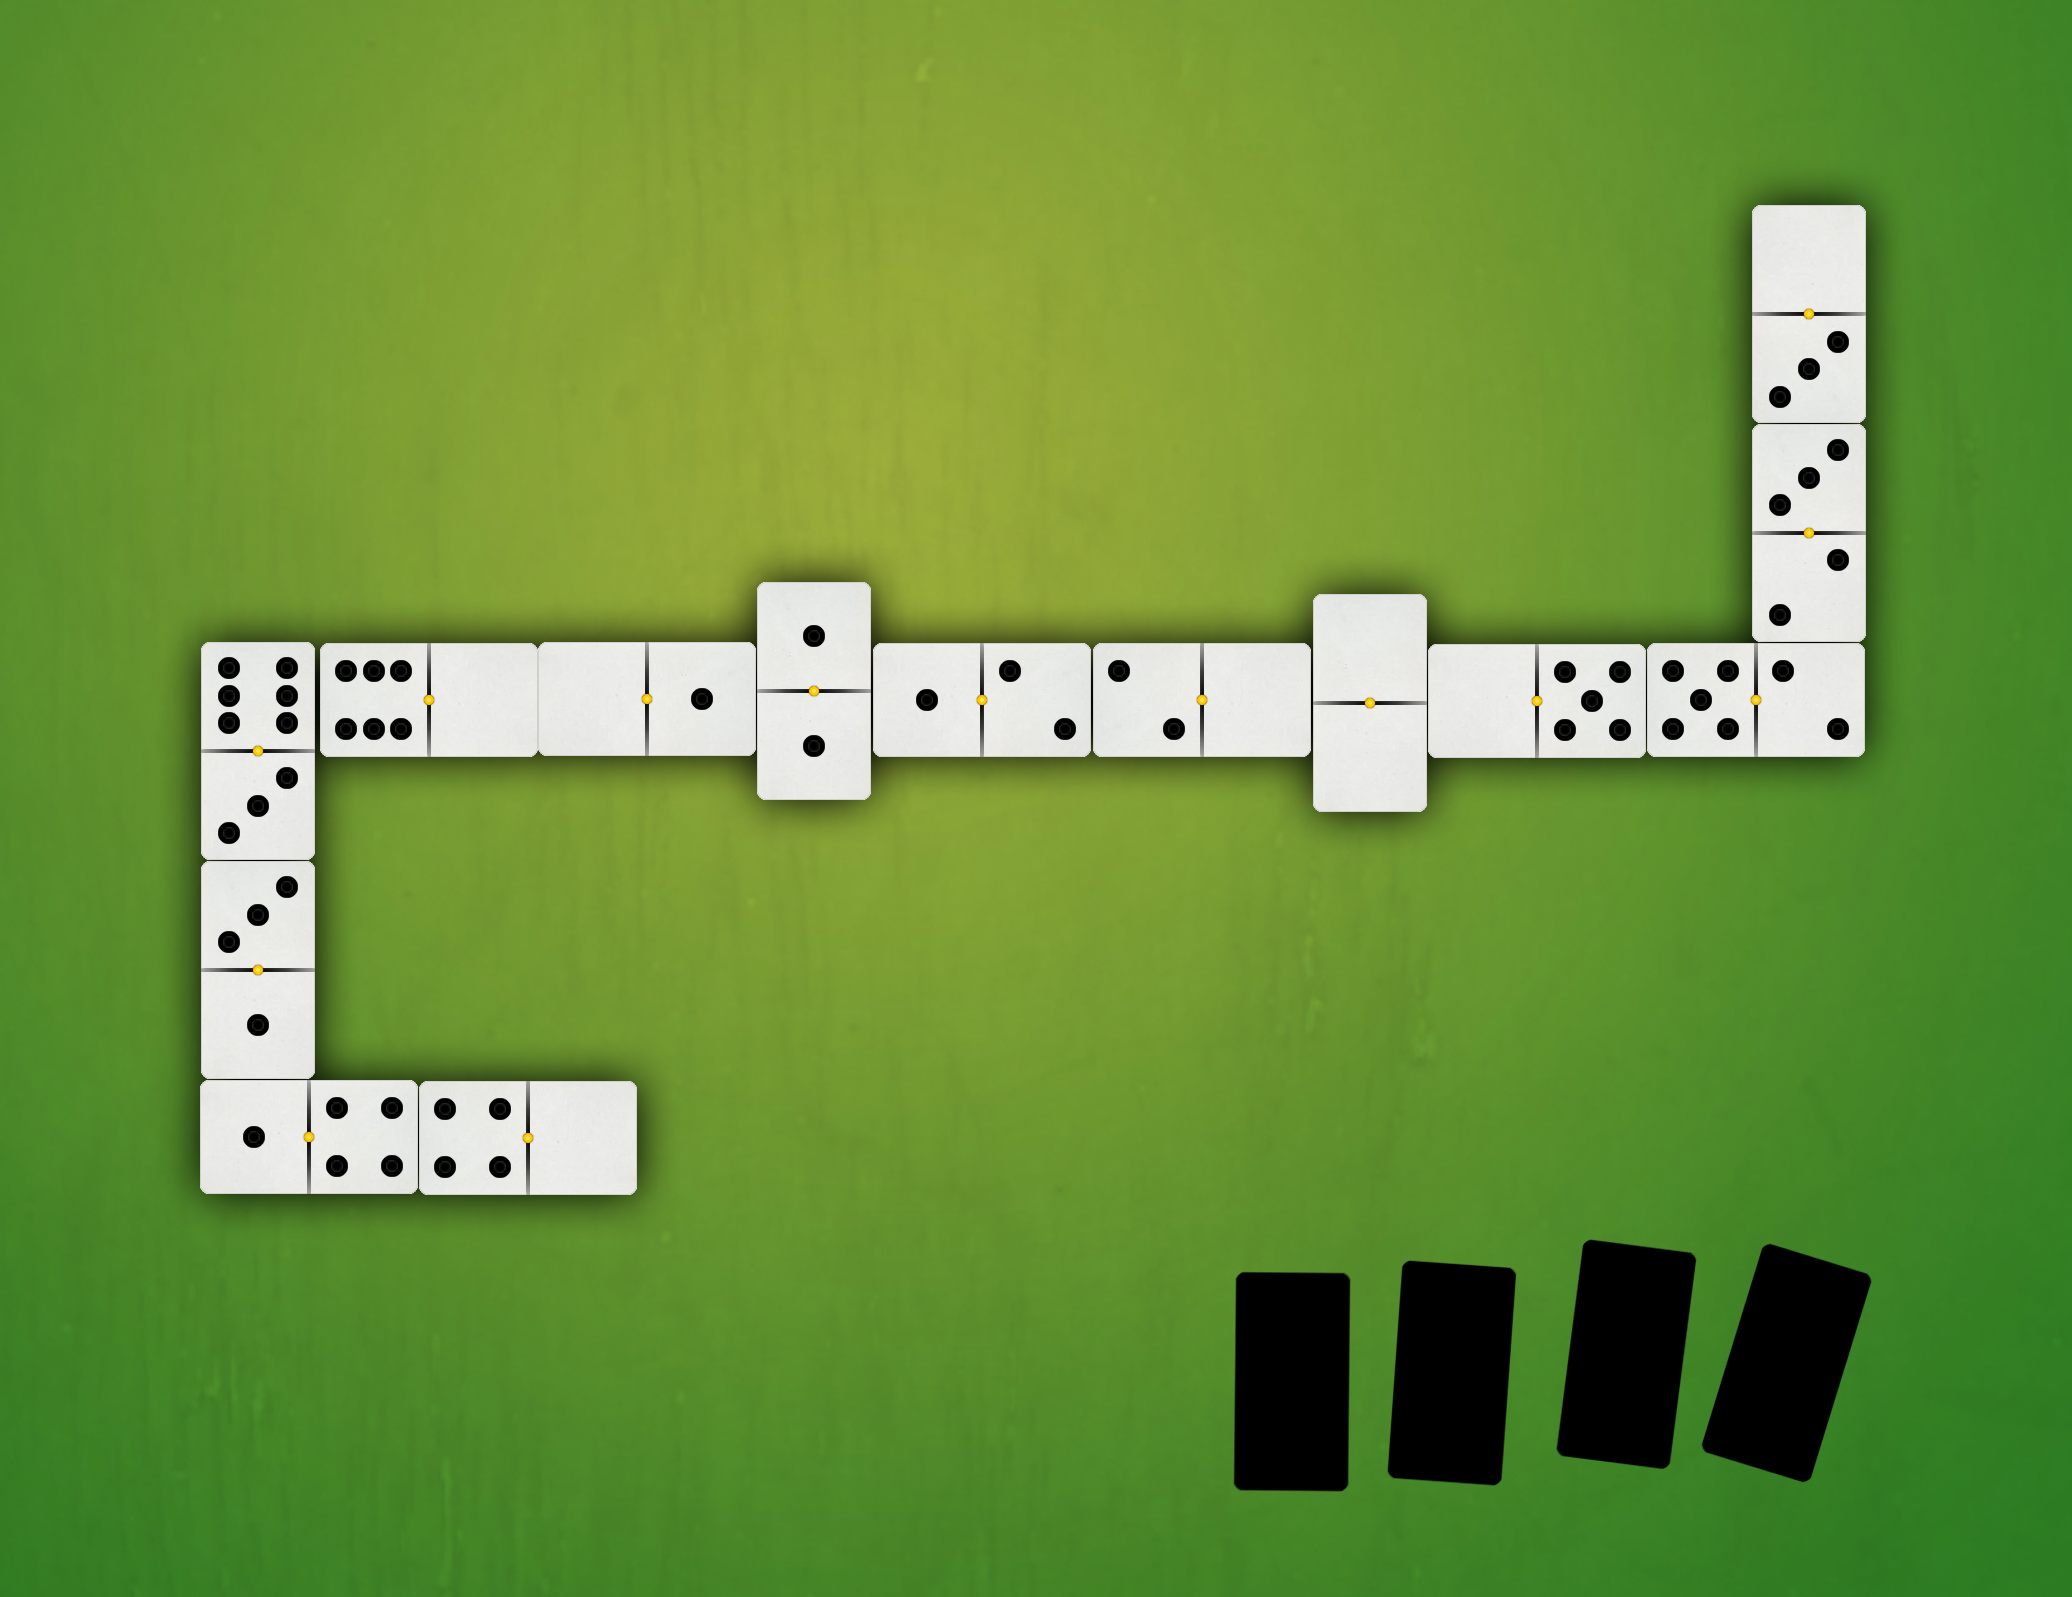
\includegraphics[scale=0.2]{cierre.png}
  \end{center}
  \caption{Ejemplo de partida terminada en cierre. Se han colocado todas las blancas, por lo que no es posible
            que algún jugador continúe la partida}
\end{figure}


La partida finaliza una vez que un equipo ha alcanzado o superado los 200 puntos. \\

\subsection{El dominó es un juego de señores}

Una gran frase que resume la filosofía del Dominó es que \emph{el dominó es un juego de señores}. Esta frase
viene a describir tanto la filosofía del juego como parte de las reglas que lo normalizan, y tendrá mucha
repercusión en cuanto al diseño del sistema experto, por lo que que pasamos a explicarla a continuación. \\

Durante el transcurso de una partida de dominó las parejas no pueden comunicar ningún tipo de información
que pueda afectar al desarrollo normal de la partida, estando totalmente prohibidos cualquier tipo de gestos
entre jugadores destinados a comunicar futuras intenciones, fichas o estrategias conjuntas. Pero existe
una excepción a esta regla. \\

La única seña o gesto válido en el juego del dominó es \emph{la pensada}. Cuando toca el turno de jugar, se tiene la
opción de pensar durante un tiempo relativamente largo para hacerle entender al compañero que se tienen
varias fichas del mismo número que va a tapar o que va a cuadrar. O por el contrario, jugar de inmediato,
sin pensar, indica que no se tienen más fichas de ese número. \\

Por lo tanto, a la hora de colocar una ficha sobre la mesa podemos --- aunque quizás tendríamos que decir que 
debemos --- comunicar cierto tipo de información a todos los jugadores de la mesa. Esta información resulta
tremendamente valiosa, y puede hacer que la partida se decante sobre un equipo o sobre el otro. \\

Hemos resaltar y aclarar que, como bien dicta la frase de que \emph{el dominó es un juego de señores},
esta seña no puede utilizarse para confundir o engañar al contrario, y en los diferentes torneos o campeonatos
de dominó supone la descalificación inmediata.


\subsection{Juego por parejas}
\label{juegoporparejas}

El juego por parejas que caracteriza el dominó internacional, a diferencia de otros tipos de modalidades,
determina las estrategias que han de seguirse para que un equipo consiga la victoria, ya que esta únicamente
se consigue trabajando en equipo; como juego de mesa por equipos, necesita imprescindible colaboración
mutua entre compañeros si se quiere conseguir la victoria común. \\

En el desarrollo de una partida los jugadores van desempeñando consecutivamente diferentes roles. Para designar
a cada jugador, es común utilizar la siguiente nomenclatura: 

\begin{description}
    \item[j1] Jugador mano que inicia la mano
    \item[j2] Jugador a la derecha del que inicia la partida
    \item[j3] Compañero del jugador que inicia la mano
    \item[j4] Compañero del jugador j2, tiene a su derecha al jugador que inicia la mano.
\end{description}

Desde el punto de vista de un jugador concreto, las posibilidades son: \\
\begin{description}
    \item[Ser el jugador mano --- jugador que inicia la partida] Este jugador es el que debe dominar la mano, ya
        que al comenzar está orientando la partida hacia la posición que le interesa; normalmente, intentará
        que el juego se mueva por el palo del que tenga más fichas. Este jugador también cuenta
        con la ventaja de que, al ser el primero que coloca ficha (salvo que no pueda jugar algún turno), es el que tiene siempre igual o menor número
        de fichas que cualquier otro jugador y puede quedarse sin ninguna antes. \\
        Por estas circunstancias, es el único jugador que puede (y debe) jugar para beneficio propio.
    \item[Segundo jugador --- jugador a la derecha del que inicia la partida] La labor de este jugador es
        evitar que el jugador mano desarrolle su estrategia, \emph{matando} las fichas con las que inicie e intentando
        reorientar la partida hacia una posición más ventajosa para él o para su compañero.
    \item[Tercer jugador --- compañero del jugador mano] Este jugador debe apoyar en la medida de lo posible
        la estrategia del jugador mano. Su juego está supeditado en origen a colocar fichas del palo con el
        que haya comenzado su compañero, con la intención de facilitarle el juego y que pueda dominar a ese palo. \\
    \item[Cuarto jugador --- a la izquierda del jugador mano] este jugador debe intentar matar las fichas que coloque
        la pareja del jugador mano, y evitar que el juego se desarrolle por el palo al que abrió el jugador mano.
\end{description}

Más tarde, dependiendo de las circunstancias de la partida, los roles
pueden ir cambiando al no poder jugar algunos jugadores sus turnos. En
todo caso, el jugador referencia será el que tenga menos fichas que el
resto, pues, si no pasara ningún turno, ganría la partida. Este puede
intentar ganarla por sí mismo si contempla la posibilidad y estima que
sus adversarios están a la espera de sus movimientos.


\subsection{Técnicas avanzadas}

% TODO

Soltar dobles

Cierres

Salida en falso

Jugar para el otro

Exceso de fichas de un tipo (de un sólo número, dobles, etc).


\section{Inteligencia artificial}

A la hora de afrontar un proyecto que simule cierto comportamiento \emph{humano}, debemos usar técnicas de Inteligencia Artificial, en busca de herramientas y metodologías que nos ayuden a afrontar este difícil problema, probablemente uno de los más complicados dentro de la Ingeniería Informática. 

\subsection{Sistemas expertos}

Para implementar la inteligencia de los contrincantes de Dominous se utilizará un
\textbf{sistema experto}~\cite{Giarratano:1989:ESP:583478}.
El desarrollo de sistemas expertos es una rama de la Inteligencia Artificial, que imita los mecanismos y la forma de
pensar de un experto en cierta materia para resolver problemas de su campo de aplicación. Esto lo hace adecuado ara un juego como el dominó, cuyas estrategias ganadoras son conocidas. Estos sistemas tiene un gran implantación en diversas ramas de la ciencia, como medicina, ingeniería o sistemas de decisiones para negocios.\\

\subsubsection{Arquitectura general}

Si consideramos el sistema una caja negra, el usuario del sistema experto sólo tiene que proporcionarle información sobre el problema y recibirá como respuesta el consejo del sistema. Para ello el sistema incorpora internamente dos elementos: la base de conocimiento (donde se almacena la información conocida) y el motor de inferencia (que permite obtener las respuestas adecuadas a partir de la información que el usuario introdujo y la base de conocimiento). La figura~\ref{fig:sistexp} muestra esta arquitectura. \\

\begin{figure}[h]
  \label{fig:sistexp}
  \begin{center}
    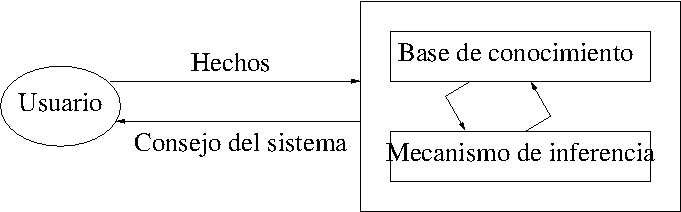
\includegraphics[scale=0.6]{sistexp.png}
  \end{center}
  \caption{Esquema conceptual de un sistema experto}
\end{figure}

\subsubsection{Desarrollo de un sistema experto}

El proceso de construcción de un sistema experto se denomina ingeniería del conocimiento. Se basa en una serie de fases que se iteran hasta conseguir un sistema adecuado (figura~\vref{fig:des_sistexp}). En una primera etapa el ingeniero de conocimiento tiene una entrevista con el experto, del que intenta obtener sus conocimientos. Después los implementa en el sistema. Y, por último, el experto evalúa el sistema. Si la evaluación no es del todo satisfactoria, se repite el proceso para refinar el resultado. \\

\begin{figure}[h]
  \label{fig:des_sistexp}
  \begin{center}
    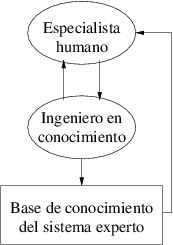
\includegraphics[scale=0.8]{des_sistexp.png}
  \end{center}
  \caption{Desarrollo de un sistema experto}
\end{figure}


\subsection{Sistemas expertos basados en reglas}

De los diversos tipos de sistemas expertos que existen~\cite{ShuHsienLiao200593} este trabajo se centrará en los sistemas expertos basados en reglas. Estos son los más adecuados para un simulador de dominó al ser este un problema con conocimiento parcial del entorno (esto es, se saben las fichas que hay en la partida, pero no qué jugador tiene cada una de ellas) y cuya inteligencia está bien estudiada y expresada en reglas concretas~\cite{Borrajo1990129}. Aún así, existe en la bibliografía una aproximación basada en redes bayesianas~\cite{PFCRoss}. \\

No este el primer trabajo en este sentido, pues existen diferentes aplicaciones de los sistemas expertos basados en reglas a todo tipos de juegos, desde sistemas en tiempo real~\cite{DBLP:conf/robocup/FathzadehMMS05} a diversos juegos de tablero (como~\cite{PFCRecio} o~\cite{PFCChaves}). \\

Los sistemas expertos basados en reglas (sistemas expertos a secas a partir de
ahora) suelen estar dividido en seis partes principales, como se
observa en la figura \ref{fig:arq_sistexp_reg}. A continuación se
detallan cada una de ellas.

\begin{figure}[h]
  \begin{center}
    \resizebox{0,8\linewidth}{!}{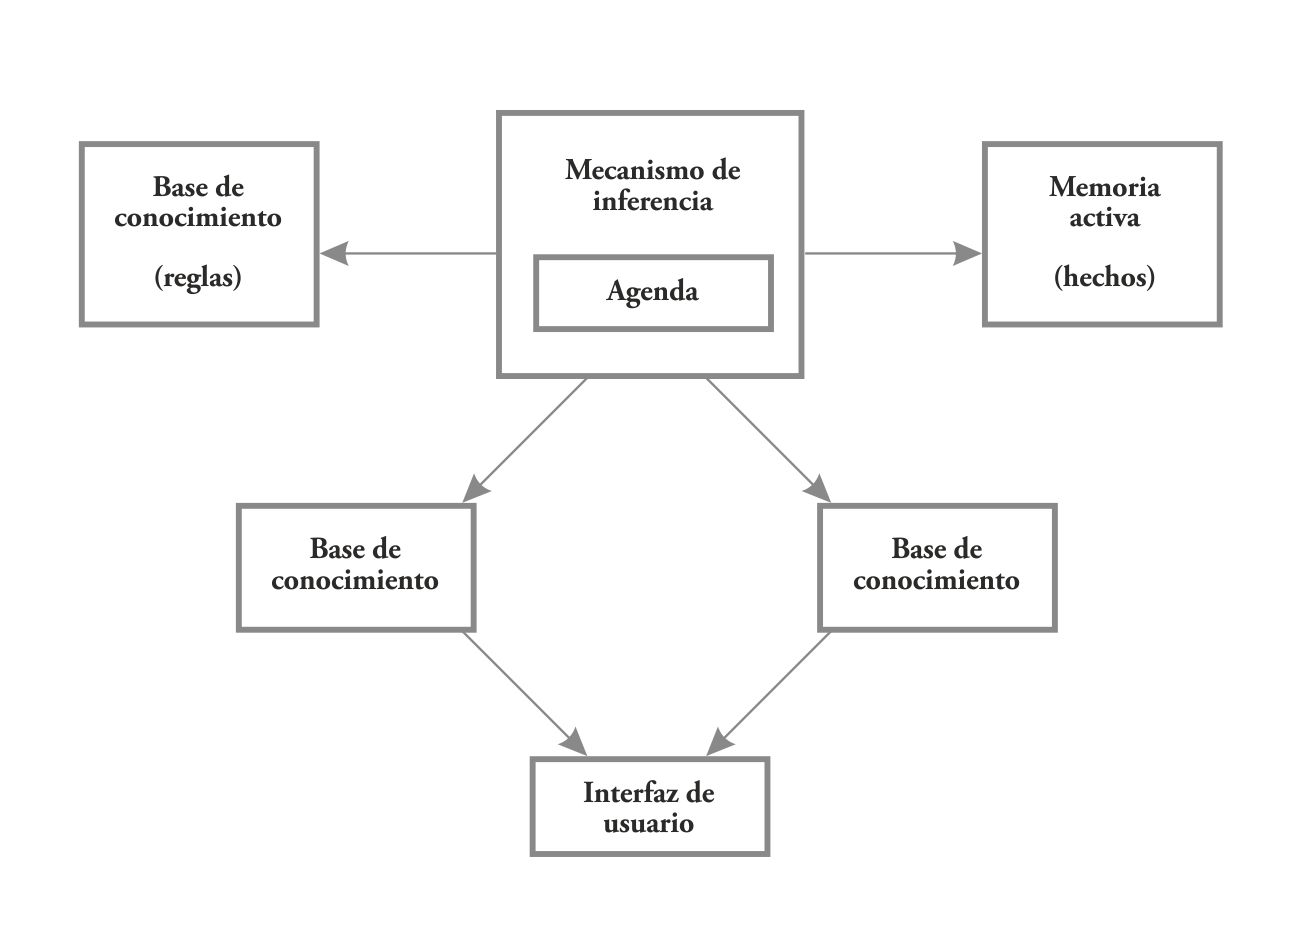
\includegraphics{arq_sistexp_reg.png}}
  \end{center}
  \caption{Arquitectura general de un sistema experto basado en reglas.}
  \label{fig:arq_sistexp_reg}
\end{figure}

\begin{description}
    \item[Base de conocimiento] Contiene conocimiento extraído del experto en forma de reglas.
    \item[Base de hechos (o Memoria activa de trabajo)] Contiene los hechos sobre un problema que se conocen.
    \item[Mecanismo de inferencia] Motor que implementa el proceso de
      razonamiento humano. Comprueba las reglas que satisface la
      memoria activa y ejecuta la que corresponda. Incluye la Agenda,
      que es el conjunto de reglas satisfechas en un momento dado.
    \item[Módulo de justificación (o Medio de explicación)] Detalla el razonamiento utilizado por
      el sistema para llegar a la conclusión proporcionada al usuario.
    \item[Medio para la adquisición de conocimiento] Permite al
      usuario introducir nuevo conocimiento en el sistema sin tener
      que mediar el ingeniero de conocimiento. El sistema suele
      recibir ejemplos para aprender de ellos.
    \item[Interfaz de usuario] Implementa la interacción del usuario con
      el sistema. La interacción la puede realizar tanto una persona
      como otro sistema que desee hacer uso del sistema experto.
\end{description}

En los siguientes apartados se desarrollan los elementos más
importantes: la memoria activa, la base de conocimiento y el motor de
inferencia.

\subsubsection{Memoria activa}

Mantiene una base de datos con la información del sistema. Esta
varía constantemente, tanto por información que se reciba
del exterior (del problema, en general) como por la información
interna que modifiquen las reglas de la base de conocimiento. \\

Está formada por dos tipos de elementos: las plantillas y los
objetos. Las plantillas definen la estructura de la información que se
almacena. En concreto especifican los atributos (del inglés
\emph{slots}) que podrán tener los objetos. Y los objetos en sí
almacenan información de acuerdo a la estructura indicada en las
plantillas.


\subsubsection{Base de conocimiento}

La base de conocimiento (también llamada \emph{sistema de producción}) de un
sistema experto es el conjunto formado por todo el conocimiento que
tiene el sistema en un momento dado. Existen sistemas en los que el
conocimiento se mantiene constante a través del tiempo (la mayoría), y
otros en los que el sistema aprende conocimiento a lo largo de su
vida. \\

El conocimiento se almacena en forma de reglas. Las reglas suelen
estar almacenadas como expresiones ``Si CONDICIÓN entonces
ACCIÓN''. Un ejemplo sería:

\begin{lstlisting}[caption={Regla en pseudocódigo}, numbers=left]
  (defrule biblioteca-regla-1
    (libro (titulo ?X) (estado retraso) (prestado-a ?Y))
    (persona (nombre ?Y) (domicilio ?Z))
    =>
    (mandar-nota-retraso ?X ?Y ?Z))
\end{lstlisting}

Esta regla en lenguaje natural se podría leer línea a línea:
\begin{lstlisting}[caption={Regla en lenguaje natural}, numbers=left]
Regla 1:
  Si
    hay un libro, titulado X, con retraso, y 
    prestado a una persona de nombre Y
    Y
    el domicilio de la persona Y es Z
  Entonces
    mandarle una nota de retraso a Y en Z del libro X
\end{lstlisting}

El libro y persona en concreto deben de estar en la memoria activa. Y
las acciones (como ``mandar-nota-retraso'' del ejemplo) se definen en
funciones escritas por el usuario. \\

En la bibliografía se suele denominar antecedente (o parte izquierda
de la regla\footnote{En inglés \emph{Left-Hand-Side}
  (\emph{L.H.S.}).}) a la condición que tiene el ``Si'', y
consecuente (o parte derecha de la regla \footnote{En inglés
  \emph{Right-Hand-Side} (\emph{R.H.S.}).}) a su acción. \\


\subsubsection{Motor de inferencia}

Su cometido es aplicar el conjunto de reglas del tipo ``si-entonces''
de la base de conocimiento al conjunto de datos que están en la
memoria activa en un momento dado. \\

La \emph{agenda} es el conjunto de reglas que se pueden ejecutar en un
momento del tiempo dado. Hay que tener en cuenta que no es lo mismo la
activación que la ejecución de una regla. La activación indica que la
regla se puede disparar (porque se satisface su condición en el
``Si''). Pero en un instante del tiempo puede haber más más de una
regla activa. Y si una de ellas se ejecuta (se dispara) puede provocar
cambios en la memoria activa e introducir o eliminar reglas de la
agenda. Además hay que tener en cuenta que en algunos sistema (sobre
todo en sistemas en tiempo real) la memoria activa puede estar
recibiendo información constantemente, lo que provoca muchas
modificaciones en la agenda tras disparar una regla y actualizar la información del mundo real. \\

En concreto, el método seguido para determinar qué regla de la agenda
se dispara se denomina \emph{estrategia de resolución de
  conflictos}. Existen muchas de ellas, que pueden ser combinadas:
asignando prioridades a las reglas, disparar primero las reglas menos
usadas (o más las usadas), disparar las reglas con mayor (o menor)
número de condiciones, etc. \\

El algoritmo más simple para implementar el motor de inferencia
(llamado \emph{regla de aproximación a la búsqueda de hechos}) sería
recorrer circularmente de modo indefinido el conjunto de reglas,
buscando reglas que se satisfagan y ejecutándolas. El problema es que
tiene una complejidad computacional de orden $O(R*F^P)$, siendo
\emph{R} el número de reglas, \emph{P} la media de comprobaciones por
el \emph{L.H.S.} de cada regla y \emph{F} la cantidad de reglas de la
base de conocimiento. Evidentemente, este orden no es deseable para
sistemas grandes, pues se dispara al incrementarse las comprobaciones
por regla, por lo que pueden necesitarse optimizaciones~\cite{springerlink:10.1007/1155698575}. Sin embargo, como veremos, es suficiente para problemas
pequeños como puede ser jugar una partida de dominó.





\chapter{Planificación}
% -*-cap2.tex-*-
% Este fichero es parte de la plantilla LaTeX para
% la realización de Proyectos Final de Carrera, protejido
% bajo los términos de la licencia GFDL.
% Para más información, la licencia completa viene incluida en el
% fichero fdl-1.3.tex

% Copyright (C) 2009 Pablo Recio Quijano 

\section{Planificación}

Para el desarrollo de \textbf{Dominous} se decidió utilizar el modelo evolutivo iterativo incremental para el ciclo de
vida del proyecto. La decisión fue tomada ya que, a pesar de tener acotado el ámbito y los requisitos del programa,
la funcionalidad concreta de cada uno de los apartados se desconocía en un principio.

El modelo iterativo incremental es un modelo de tipo evolutivo que está basado en varios ciclos cascada realimentados aplicados
repetidamente, con una filosofía iterativa. Como se comenta en CITE, al final de cada iteración se le
realiza una entrega al cliente final; en este caso, el cliente ha sido el tutor del proyecto, que a cada iteración iba
dictando las líneas maestras generales a tomar a cada nuevo paso.

Las ventajas de utilizar un modelo iterativo incremental son básicamente los siguientes:
\begin{enumerate}
    \item Construir un sistema pequeño es siempre menos costoso en términos de riesgo.
    \item Al ir desarrollando parte de las funcionalidades, es más fácil determinar si los requerimientos
            planeados para los niveles subsiguientes son correctos.
    \item Si se comete algún error grave, sólo la última iteración necesita ser descartada.
    \item Reduciendo el tiempo de desarrollo de un sistema (en este caso en incremento del sistema) decrecen las
            probabilidades que esos requerimientos de usuarios puedan cambiar durante el desarrollo.
    \item Los errores de desarrollo realizados en un incremento, pueden ser arreglados antes del comienzo del próximo incremento.
\end{enumerate}

El proyecto \textbf{Dominous} consta de tres subsistemas que son los que ocupan el grueso del desarrollo:
\begin{enumerate}
    \item El primero es el motor de la partida: Controla los jugadores, las fichas en la mesa, la partida, situaciones irregulares
            y cualquier otro elemento referente únicamente al ámbito del dominó.
    \item Por otro lado está el motor gráfico, que será la interfaz entre la partida y el usuario, permitiendo el movimiento
            fluído por las diferentes secciones del programa e interactuando de forma directa con el motor de la partida,
            mostrando las fichas actuales y habilitando la interacción del jugador con el mundo.
    \item Y por último tenemos el motor de Inteligencia Artificial. Este motor será el que alimente la inteligencia
            y las acciones y decisiones de los jugadores controlados por el ordenador.

\subsection{Incrementos realizados}

A continuación se citan los diferentes incrementos que se han ido realizando en el desarrollo del proyecto.

\subsubsection{Preliminares}

El primer paso a la hora de enfrentarse a un proyecto es decidir las herramientas que vamos a utilizar. En principio se
pensó utilizar el lenguage C++ por dos sencillas razones:
\begin{enumerate}
    \item Por un lado es un lenguaje que hemos aprendido en la carrera, se ha utilizado en varias asignaturas de
            diferentes ramas, con lo cual la comodidad y familiaridad que podemos tener a la hora de programar
            es un punto importante a tener en cuenta.
    \item Tampoco podemos olvidar que, al ser un lenguaje compilado, la velocidad de ejecución que se consigue
            es interesante, y mucho más tratándose de temas como la inteligencia artificial (donde puede ser
            necesario un uso intensivo de los recursos del sistema) o el desarrollo de videojuegos (en el que
            la potencia del ordenador repercute en una mejor experiencia del usuario)
\end{enumerate}
    


\chapter{Análisis}
% ANÁLISIS

\section{Toma de requisitos}

En el desarrollo de esta aplicación la toma de requisitos se hizo mediante reuniones con el tutor del proyecto,
que realizaba el papel de cliente potencial de la misma. Después de varias reuniones se obtuvo el listado de requisitos
que se muestra en las siguientes secciones:


\subsection{Requisitos de interfaces externas}

En este apartado se van a describir los requisitos de conexión entre el software y el hardware, así como la interfaz
del usuario.\\

De la interfaz entre el software y el hardware se encarga la librería SDL, mediante el wrapper pygame --- y por encima
la capa que añade Gloss--- que, al ser un sistema preestablecido, no será necesario analizarlo ni diseñarlo,
simplemente haremos uso de él.\\

Así que pasamos a definir el interfaz entre el videojuego y el usuario. Todas las ventanas de la aplicación podrán
ser mostradas a pantalla completa o en formato de ventana con una resolución de 800 por 600 píxeles. A
continuación se definen las distintas ventanas con las que el usuario se puede encontrar:

\begin{description}
    \item[Ventana de introducción] Esta primera ventana mostrará únicamente el logotipo de Dominous, situando al usuario
            en contexto para iniciarlo en la ejecución del programa
    \item[Ventana del menú principal] La ventana del menú principal muestra el menú de inicio de Dominous, en el que
            el usuario podrá elegir entre las opciones más generales del juego, entre las que se encuentran:
            \begin{itemize}
                \item Partida clásica
                \item Laboratorio
                \item Opciones
                \item Tutorial
                \item Salir
            \end{itemize}
            Este menú y los siguientes que se describan serán completamente manejados por el ratón y bastará
            un clic encima de una opción para acceder a ella.
    \item[Ventana de selección de personaje] Esta ventana mostrará una interfaz que permite al usuario elegir los
            diferentes participantes que se enfrentarán en la siguiente partida. En caso del modo laboratorio
            se elegirán los cuatro jugadores, y en caso de partida clásica serán tres jugadores controlados por
            el ordenador más el jugador humano.
    \item[Ventana de partida] Esta será la ventana principal de todo el juego. Mostrará una partida de dominó
            de dos equipos, el tablero e información de la partida, e irá actualizando el tablero según se vaya
            desarrollando la misma partida. Mediante la pulsación de la tecla ESC o clic sobre el botón menú se
            desplegará el menú interno de la partida, que permitirá abandonarla a pesar de no haberse terminado
            la partida actual.
    \item[Ventana de laboratorio] La ventana de laboratorio proporciona una interfaz para que el usuario de la
            aplicación pueda generar un conjunto elevado de partidas entre dos equipos definidos, con la idea
            de poder decidir qué pareja presenta las mejores características de Inteligencia Artificial.
    \item[Ventana del modo tutorial] Por último la ventana del modo tutorial mostrará al usuario información sobre
            el juego del dóminó mediante un conjunto de presentaciones, para que el mismo usuario pueda aprender
            más sobre el mundo del dominó sin necesidad de salir de la aplicación.
\end{description}


\subsection{Requisitos funcionales}

Los requisitos funcionales que el sistema debe ofrecer al usuario son los siguientes:
\begin{itemize}
    \item Poder jugar una partida de dominó con tres jugadores más controlados por el ordenador.
    \item Enfrentar a dos parejas de jugadores controlados por ordenador, haciendo que jueguen un gran número
            de partidas seguidas en modo automático (esto es, sin visualizar la partida que se desarrolla y
            mostrando únicamente las victorias), con la finalidad de poder decidir qué pareja posee una
            inteligencia artificial más avanzada.
    \item Acceder al modo tutorial, para realizar un aprendizaje de las normas, técnicas y usos del dominó.
    \item Cambiar el tipo de juego para que cuatro jugadores manejados por la máquina puedan desarrollar una
            partida en modo visual.
    \item Seleccionar otro tema gráfico para que, tanto fichas como tablero como otros elementos gráficos, cambien
            a gusto del usuario, eligiendo entre cierto abanico de temas.
    \item Cambiar de modo ventana a modo pantalla completa.
\end{itemize}


\subsection{Requisitos de rendimiento}

El rendimiento de la aplicación debe ser tal que permita un desempeño agradable de la partida. Este requisito
hace referencia principalmente a los siguientes asuntos:
\begin{itemize}
    \item El sistema de inteligencia artificial debe ser lo suficientemente ágil y estar ajustado y
            perfeccionado para que los tiempos empleados en cálculos de toma de decisiones no ralenticen
            la partida. Se cuenta como asunto el que, en el desarrollo de una partida de dominó, los tiempos de
            espera también se interpretan, por lo que debemos realizar los cálculos dentro de un cierto
            margen de tiempo.
    \item Por otro lado, el motor gráfico debe estar optimizado para que el usuario no aprecie movimientos
            bruscos a la hora de manejar la aplicación. No olvidemos que estamos desarrollando un videojuego,
            así que el programa debe mostrar cierta agilidad a la hora de realizar movimientos y transiciones
            entre los diferentes estados de la partida, incluyendo menús, fichas, o asuntos relativos a la
            interfaz, como puede ser el arrastrar una ficha a su lugar correspondiente.
\end{itemize}

Es importante recordar en todo momento que estamos desarrollando una aplicación en tiempo real, por lo que
debe primar la velocidad sobre otros factores como el consumo de memoria principal.


\subsection{Restricciones de diseño}
Como bien comentábamos en el punto anterior, a la hora de realizar el diseño de la aplicación tienen que
primar los tiempos de respuesta sobre el consumo de recursos de la memoria principal o secundaria. Esta
es la principal restricción que tendrá el diseño de nuestra aplicación.\\

Los videojuegos están pensados para ejecutarse como aplicación principal, no para compartir recurssos
con otros programas; por esta razón se permite que consuman muchos recursos.


\subsection{Requisitos del sistema software}

La aplicación debe cumplir con los siguientes requisitos de sistema:
\begin{itemize}
    \item La aplicación debe ejecutarse de forma multiplafatorma, incluyendo como mínimo los sistemas operativos:
        \begin{itemize}
            \item En Microsoft Windows --- Realizándose las pruebas en la versión Windows 7 con las últimas actualizaciones
            \item En sistemas GNU/Linux --- Utilizando la distribución Ubuntu en su versión 10.04 con su instalación
                    por defecto y con todas las actualizaciones del sistema.
        \end{itemize}
    \item El código de la aplicación no debe ser dependiente del sistema operativo en el que se desarrolle la aplicación,
            y debe ser un código mantenible y fácilmente ampliable para futuras mejoras y versiones.
\end{itemize}

\section{Modelo de casos de uso}

Para describir los comportamientos que tendrá el sistema, utilizaremos el lenguaje guaje de modelado de sistemas UML;
éste representa los requisitos funcionales de todo el sistema, centrándose en qué hace pero no en cómo lo hace.\\

A continuación describimos uno por uno cada caso de uso.

\subsection{Diagrama de casos de uso}

Como primer paso, debemos mostrar el diagrama de casos de uso que representa la funcionalidad completa de la aplicación.
El esquema utilizado es el siguiente:
\begin{enumerate}
    \item Identificar los usuarios del sistema y sus posibles roles.
    \item Para cada rol definido, identificar todas las formas que tiene de interactuar con el sistema. En el caso
            de Dominous, existe un único rol de acceso a la aplicación, por lo que la especificación de usuario
            será única.
    \item Crear todos los casos de uso para poder describir los objetivos que se desean cumplir.
    \item Estructurar y definir esos casos de uso.
\end{enumerate}

\begin{figure}[h]
  \label{diagrama-casos-uso}
  \begin{center}
    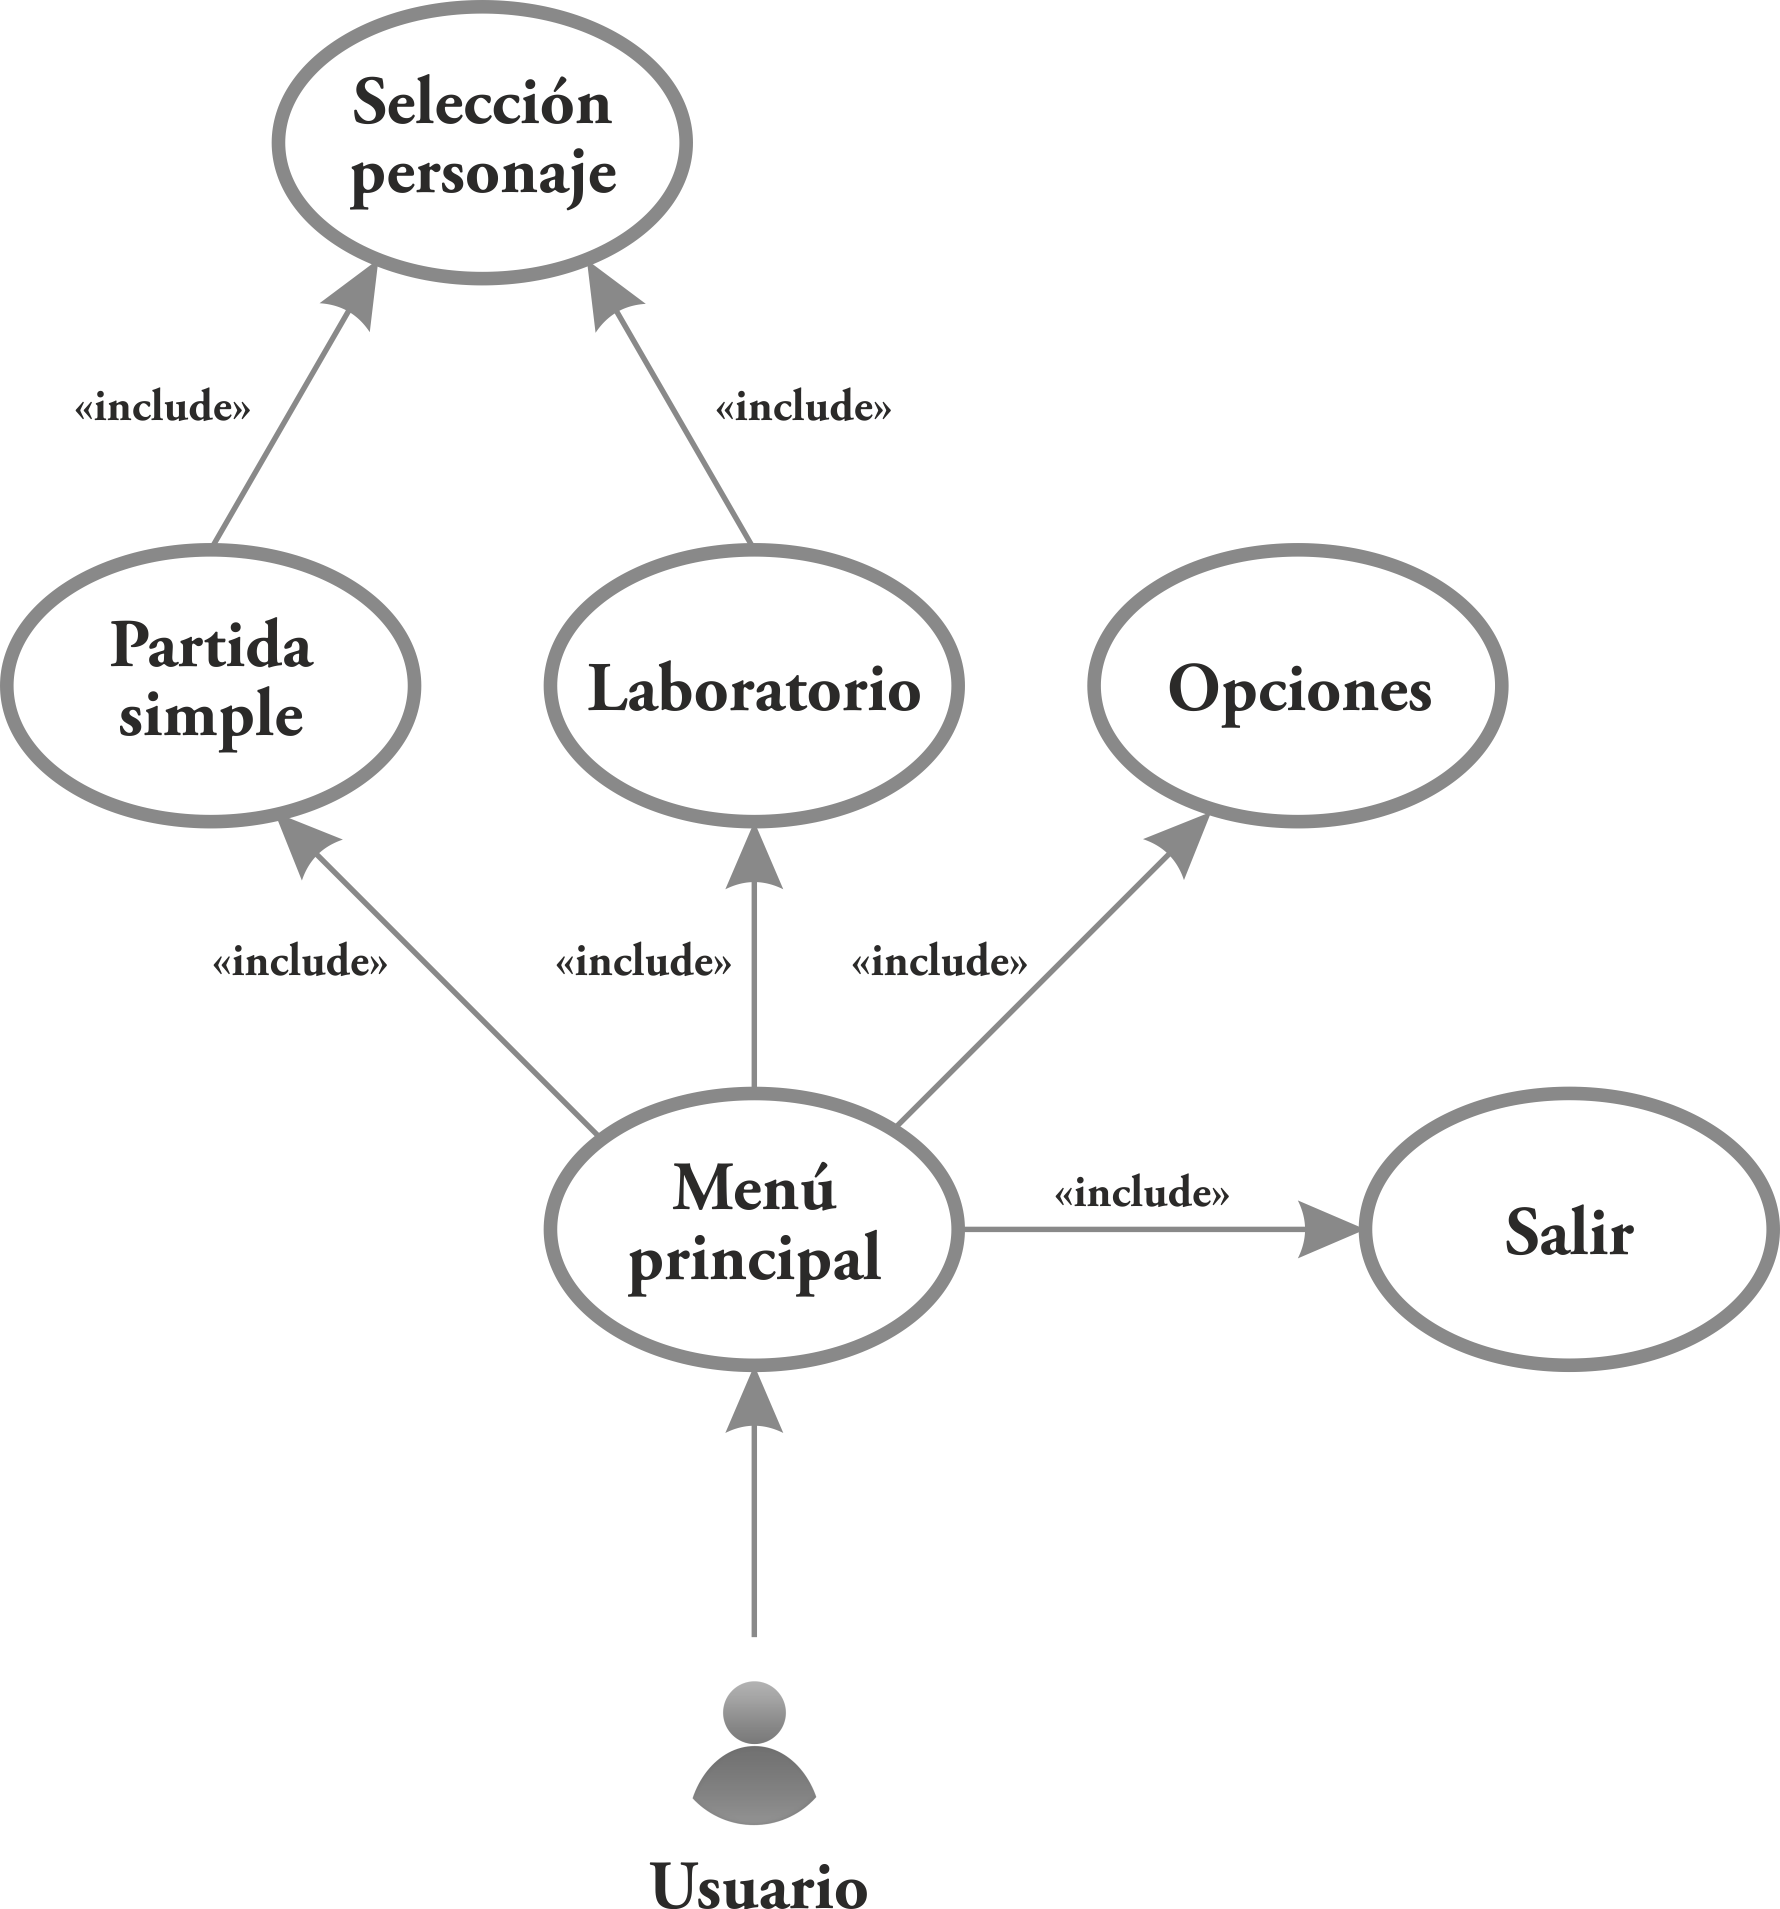
\includegraphics[scale=0.7]{diagrama_casos_de_uso.png}
  \end{center}
  \caption{Diagrama de casos de uso del sistema}
\end{figure}


\subsection{Descripción de los casos de uso}

A continuación pasamos a la descripción de los casos de uso. Para ello se va a utilizar una notación formal
usando plantillas, con la intención y finalidad de que este texto sea legible y comprensible por
un usuario que no sea experto.

\subsubsection{Caso de uso: Menú principal}

\begin{description}
    \item[Caso de uso] Menú principal
    \item[Descripción] Se muestra el menú principal de la aplicación, desde donde es posible acceder a los
        diferentes modos de juego y a las opciones.
    \item[Actores] Usuario
    \item[Precondiciones] Ninguna
    \item[Postcondiciones] Ninguna
    \item[Escenario principal] $\quad$
        \begin{enumerate}
            \item El sistema muestra el menú principal del juego en la pantalla
            \item El usuario selecciona el modo \textbf{partida simple}
            \item El sistema inicia el modo de elección de jugadores
        \end{enumerate}
    \item[Extensiones --- flujo alternativo] $\quad$
        \begin{description}
            \item[*a ] El usuario cierra la ventana de la aplicación y sale de la aplicación
            \item[2a ] El usuario pulsa sobre el botón de laboratorio, dirigiéndose a ese apartado de la aplicación
            \item[2b ] El usuario pulsa el botón de tutorial, dirigiéndose a ese apartado de la aplicación
            \item[2c ] El usuario pulsa sobre las opciones, dirigiéndose a ese apartado de la aplicación
            \item[2d ] El usuario pulsa sobre el botón de salir, cerrándose la aplicación
        \end{description}
   
\end{description}

\subsubsection{Caso de uso: Salir}

\begin{description}
    \item[Caso de uso] Salir.
    \item[Descripción] Primeramente se muestra la pantalla de información de la aplicación --- con más datos
            sobre desarrolladores, licencias y cualquier otra información que pueda resultar de interés para
            el usuario.
    \item[Actores] Usuario.
    \item[Precondiciones] Ninguna.
    \item[Postcondiciones] Se sale de la aplicación.
    \item[Escenario principal] $\quad$
        \begin{enumerate}
            \item El sistema muestra la pantalla de información.
            \item El usuario pulsa sobre cualquier lugar de la aplicación.
            \item La aplicación se cierra.
        \end{enumerate}
    \item[Extensiones --- flujo alternativo] $\quad$
        \begin{description}
            \item[*a ] El usuario cierra la ventana de la aplicación y sale de la aplicación.
        \end{description}
\end{description}
 

\subsubsection{Caso de uso: Partida simple}

\begin{description}
    \item[Caso de uso] Partida simple.
    \item[Descripción] El usuario pulsa el botón partida simple con la intención de comenzar una partida
            de dominó con las opciones por defecto, esto es, jugando por parejas con tres jugadores más
            controlados por el ordenador. El usuario selecciona su pareja de equipo y sus dos adversarios, y
            da comienzo la partida
    \item[Actores] Usuario.
    \item[Precondiciones] Ninguna.
    \item[Postcondiciones] Se jugará una partida de \textbf{Dominous}
    \item[Escenario principal] $\quad$
        \begin{enumerate}
            \item El usuario desea jugar una partida.
            \item El usuario selecciona la opción de menú \textbf{partida simple}.
            \item \texttt{include} \textsc{selección de jugadores}.
            \item El sistema inicializa y muestra la partida actual por pantalla
            \item Por cada mano que se desarrolle:
                \begin{enumerate}
                    \item El usuario y el sistema interactúan durante la partida.
                    \item El sistema muestra quién ha ganado la mano.
                \end{enumerate}
            \item El sistema muestra quién ha ganado al final de la partida.
            \item El sistema cierra la partida y muestra de nuevo el menú principal.
        \end{enumerate}
    \item[Extensiones --- flujo alternativo] $\quad$
        \begin{description}
            \item[*a ] El usuario cierra la ventana de la aplicación y sale de la aplicación.
            \item[2a ] El usuario pulsa sobre cualquier otra opción del menú que no sea la de realizar una
                    partida simple --- se rompe el flujo y se redirige al usuario a la opción elegida. 
            \item[5a ] El usuario pulsa el botón de menú y pulsa en salir de la partida. Se termina la partida
                    actual y se vuelve al menú principal.
        \end{description}
\end{description}

\subsubsection{Caso de uso: Laboratorio}

\begin{description}
    \item[Caso de uso] Laboratorio
    \item[Descripción] El usuario desea realizar pruebas y análisis sobre las diferentes habilidades de cada jugador
            controlado por la Inteligencia Artificial del programa, enfrentando a dos equipos de jugadores a un alto
            número de partidas, y calculando el mejor equipo según el número de victorias alcanzadas.
    \item[Actores] Usuario.
    \item[Precondiciones] Ninguna.
    \item[Postcondiciones] Se realizará una competición a 100 partidas, cada partida jugada a 200 puntos, enfrentando
            a las dos parejas de jugadores seleccionados previamente.
    \item[Escenario principal] $\quad$
        \begin{enumerate}
            \item El usuario desea acceder al modo laboratorio.
            \item El usuario selecciona la opción de menú \textbf{laboratorio}.
            \item \texttt{include} \textsc{selección de jugadores}.
            \item El sistema comienza con los enfrentamientos entre ambas parejas
            \item El sistema finaliza los enfrentamientos y destaca al equipo ganador
            \item El sistema cierra el modo laboratorio y muestra de nuevo el menú principal.
        \end{enumerate}
    \item[Extensiones --- flujo alternativo] $\quad$
        \begin{description}
            \item[*a ] El usuario cierra la ventana de la aplicación y sale de la aplicación.
            \item[*b ] El usuario pulsa el botón de salir del modo laboratorio y se vuelve al menú principal.
            \item[2a ] El usuario pulsa sobre cualquier otra opción del menú que no sea la de realizar una
                    partida simple --- se rompe el flujo y se redirige al usuario a la opción elegida.
            \item[4a ] El usuario pulsa el botón de pausa --- se realiza una pausa en el desarrollo de las
                    partidas, hasta el momento en el que el usuario vuelve a pulsar el botón de pausa y se
                    reanudan los enfrentamientos
            \item[4b ] El usuario pulsa el botón de reiniciar --- se resetean a cero los contadores de partidas,
                    puntos y cualquier otra estadística sobre la que se realice el conteo, y se comienza a
                    desarrollar de nuevo un nuevo conjunto de enfrentamientos.
            \item[6a ] El usuario pulsa el botón de salir del modo laboratorio y se vuelve al menú principal.
        \end{description}
\end{description}

\subsubsection{Caso de uso: Opciones}

\begin{description}
    \item[Caso de uso] Opciones
    \item[Descripción] El usuario decide cambiar alguna elemento de la configuración con la que se desarrollan
            las partidas y que modifican el comportamiento transversal de la aplicación.
    \item[Actores] Usuario.
    \item[Precondiciones] Ninguna.
    \item[Postcondiciones] Se cambian las opciones que se desean modificar por parte del usuario, y se vuelve
            de nuevo al menú principal.
    \item[Escenario principal] $\quad$
        \begin{enumerate}
            \item El usuario desea acceder y cambiar las opciones del juego.
            \item El usuario selecciona la opción de menú \textbf{opciones}.
            \item El sistema muestra todas las opciones.
            \item El usuario pulsa en volver.
            \item El sistema guarda en la configuración general del juego las opciones seleccionadas, para
                    que en posteriores ejecuciones se mantengan las mismas opciones previamente seleccionadas.
            \item El sistema muestra de nuevo el menú principal.
        \end{enumerate}
    \item[Extensiones --- flujo alternativo] $\quad$
        \begin{description}
            \item[*a ] El usuario cierra la ventana de la aplicación y sale de la aplicación.
            \item[*b ] El usuario pulsa el botón volver y se retorna al menú principal.
            \item[2a ] El usuario pulsa sobre cualquier otra opción del menú que no sea la de realizar una
                    partida simple --- se rompe el flujo y se redirige al usuario a la opción elegida.
            \item[3a ] El usuario pulsa en \textbf{modo de juego} --- el sistema va rotando entre las diferentes
                    opciones de juego, que son dos: \textbf{modo de juego un jugador} (el jugador humano participa
                    de la partida) y \textbf{modo de juego solo computadora} (todos los jugadores participantes
                    estarán controlados por la máquina).
            \item[3b ] El usuario pulsa en \textbf{tema gráfico} --- el sistema va rotando entre los distintos
                    temas gráficos que están instalados en la aplicación, y que más tarde cambiarán el aspecto
                    visual de la partida.
            \item[3c ] El usuario pulsa en \textbf{velocidad de juego} --- el sistema permite elegir entre tres
                    tipos de velocidades para la partida: \textbf{velocidad normal}, en el que la partida
                    transcurre a una velocidad pausada y cómoda, \textbf{velocidad rápida}, en el que los jugadores
                    manejados por la máquina colocan las fichas sin realizar pausas para pensar, y \textbf{velocidad
                    extra rápida}, en el que, además de no realizar pausa, las fichas se mueven cuatro veces
                    más rápido de la velocidad normal de juego.
            \item[3d ] El usuario pulsa en \textbf{modo ventana} --- El sistema permite cambiar entre dos modos
                    de visualización del juego: \textbf{modo ventana}, en el que la aplicación se muestra dentro de
                    una ventana controlada por el gestor de ventanas nativo del sistema, y el \textbf{modo pantalla
                    completa}, donde la acción ocupa toda la pantalla activa del usuario.
        \end{description}
\end{description}

\subsubsection{Caso de uso: Selección de personaje}

\begin{description}
    \item[Caso de uso] Selección de personaje.
    \item[Descripción] El usuario desea seleccionar los jugadores que participarán en el siguiente juego
            a desarrollar, ya sea \textbf{partida simple} o modo \textbf{laboratorio}.
    \item[Actores] Usuario.
    \item[Precondiciones] El usuario ha pulsado previamente una de estas dos opciones del menú principal:
            \textbf{partida simple} o modo \textbf{laboratorio}.
    \item[Postcondiciones] Se guardará en configuración los jugadores seleccionados por el usuario para el
            posterior desarrollo del juego.
    \item[Escenario principal] $\quad$
        \begin{enumerate}
            \item El usuario debe seleccionar los personajes que participarán en el juego
            \item El sistema muestra los jugadores actuales.
            \item El usuario selecciona los personajes que jugarán la partida o partidas siguientes.
            \item El usuario está satisfecho con su elección y pulsa el botón de jugar.
            \item El sistema guarda la información de los jugadores seleccionados.
            \item El sistema pasa al siguiente paso, que puede ser \textbf{partida simple} o modo
                    \textbf{laboratorio}, dependiendo del estado de la precondición.
        \end{enumerate}
    \item[Extensiones --- flujo alternativo] $\quad$
        \begin{description}
            \item[*a ] El usuario cierra la ventana de la aplicación y sale de la aplicación.
            \item[*b ] El usuario pulsa el botón de volver, con lo que se retorna al menú principal.
            \item[3a ] El usuario pulsa sobre cada jugador, con la intención de seleccionar aquellos que
                    jugarán la partida o partidas siguientes. A cada pulsación, el sistema mostrará el
                    siguiente jugador existente en el sistema, de forma cíclica.
        \end{description}
\end{description}

\section{Modelo conceptual de datos}

Este apartado del análisis sirve para especificar los requisitos del sistema y las relaciones estáticas que
existen entre ellos. \\

Para este fin se utiliza como herramienta los \textbf{diagramas de clase}. En estos diagramas se representan
las clases de objetos, las asociaciones entre dichas clases, los atributos que componen las clases y las
relaciones de integridad.

\subsection{Diagrama de clases conceptuales}

En este apartado se presenta una lista de las principales clases que formarán parte del sistema y una pequeña
descripción sobre la labor que desempeña cada una.

\begin{description}
    \item[AI]
    \item[Config]
    \item[Dominoes]
    \item[Dominous]
    \item[Engine]
    \item[Finish]
    \item[Gloss]
    \item[Intro]
    \item[Lab]
    \item[Menu]
    \item[Selectplayers]
    \item[Sound]
    \item[Tools]
    \item[Tutorial]
\end{description}


\chapter{Diseño}
% -*-cap2.tex-*-
% Este fichero es parte de la plantilla LaTeX para
% la realización de Proyectos Final de Carrera, protegido
% bajo los términos de la licencia GFDL.
% Para más información, la licencia completa viene incluida en el
% fichero fdl-1.3.tex

% Copyright (C) 2009 Pablo Recio Quijano 

\section{Introducción}

El primer paso que vamos a dar para describir el diseño de la aplicación será describir los requisitos del
sistema necesarios para poder ejecutar la aplicación, y posteriormente comentaremos las herramientas que se
van a usar para el desarrollo de la aplicación.

\section{Definición de los requisitos del sistema}

Los requisitos hardware y software necesarios para poder ejecutar con soltura la aplicación son los siguientes:

\begin{itemize}
	\item Sistema operativo Microsoft Windows en su versión Windows 7, o sistemas basados en GNU/Linux tales como
		la distribución Ubuntu en su versión 10.04.
	\item Últimas actualizaciones del sistema instaladas, drivers y demás aplicaciones propias del sistema
		configuradas correctamente.
	\item Procesador igual o superior a 1,6 GHz.
	\item Memoria RAM igual o superior a 512 MB
	\item Tarjeta gráfica con aceleración 3D con un mínimo de 128 MB
	\item En versiones basadas en Linux, se requieren las siguientes librerías:
		\begin{itemize}
			\item python-pygame
			\item python-setuptools
			\item PyOpenGL
			\item PyOpenGL-accelerate
		\end{itemize}
	\item Por otro lado, si el sistema está basado en Microsoft Windows, necesitaremos:
		\begin{itemize}
			\item Pygame
			\item Python OpenGL and Gloss
		\end{itemize}
\end{itemize}

\section{Herramientas utilizadas}

\subsection{Librería gráfica}

Para todo el tema del aspecto gráfico, mi tutor me recomendó que utilizara las librerías SDL\footnote{Simple
Directmedia Layer}, ya que son unas librerías orientadas al desarrollo de videojuegos con varias particularidades:
\begin{itemize}
    \item Son completas, ya que permiten gestionar operaciones de dibujo en dos dimensiones, efectos de
            sonido y música, carga y gestión de imágenes, subsistemas de control de métodos de entrada,
            etcétera, por lo que contamos con una solución global para desarrollar videojuegos.
    \item Están programas en C, por lo que se puede esperar un buen rendimiento de las librerías en
            diferentes entornos.
    \item Multiplataforma: es compatible oficialmente con los sistemas Microsoft Windows, GNU/Linux,
            Mac OS y QNX, además de otras arquitecturas y sistemas menos comunes como Sega Dreamcast, Sony PSP,
            WebOS, Google Android o Symbian entre otros.
    \item Tampoco hay que mantener al margen la característica de que cuenta con wrappers a otros lenguajes
            de programación como entre los que se encuentran C++, Ada, C\#, BASIC, Erlang, Lua, Java o Python, por
            lo que nos da bastante libertad para elegir un lenguaje de programación principal
    \item Publicado bajo licencia LGPL, con todas las ventajas que conlleva.
    \item Y por último no hay que menospreciar que mi tutor emplea SDL a la hora de impartir la asignatura
            de diseño de videojuegos, y contar con esa base de conocimiento nos ayudará a desarrollar más rápidamente
            y solucionar antes nuestros posible problemas.
\end{itemize}

\begin{figure}[h]
  \label{logo-sdl}
  \begin{center}
    
\includegraphics[scale=0.5]{SDL.png}
  \end{center}
  \caption{Logotipo de la librería Simple DirectMedia Layer}
\end{figure}

En este aspecto, la utilización de las librerías SDL estaba clara. Potencia, comodidad, multiplataforma y con la posibilidad
de utilizar diferentes lenguajes de programación.\\

\subsection{Lenguaje de programación}

Una vez que tocamos el tema de los lenguajes de programación, entra en escena la problemática sobre qué lenguaje
utilizar. En principio se pensó emplear el lenguaje C++ por dos sencillas razones:

\begin{enumerate}
    \item Por un lado es un lenguaje que hemos aprendido en la carrera, se ha utilizado en varias asignaturas de
            diferentes ramas, con lo cual la comodidad y familiaridad que podemos tener a la hora de programar
            es un punto importante a tener en cuenta.
    \item Tampoco podemos olvidar que, al ser un lenguaje compilado, la velocidad de ejecución que se consigue
            es interesante, y mucho más tratándose de temas como la inteligencia artificial (donde puede ser
            necesario un uso intensivo de los recursos del sistema) o el desarrollo de videojuegos (en el que
            la potencia del ordenador repercute en una mejor experiencia del usuario)
\end{enumerate}

Pero hay que detenerse un momento y pensar en la naturaleza del proyecto. Aunque el programa a desarrollar sea un
videojuego, no hay que olvidar que hay diferentes tipos de juegos, que pueden condicionar o influir en nuestra forma
de programarlo. En el caso del dominó, lo primero que debemos tener en cuenta es que el apartado gráfico no va a
requerir de una gran potencia o despliegue de efectos: el dominó es un juego pausado y a diferencia de otros
videojuegos lo importante en este caso es mostrar al usuario la información de la partida de una forma clara y sencilla,
para que el jugador evalúe las posibilidades de acción y actúe en consecuencia.\\

\begin{figure}[h]
  \label{logo-python}
  \begin{center}
    
\includegraphics[scale=0.3]{python.png}
  \end{center}
  \caption{Logotipo de Python - Copyright Python Software Foundation}
\end{figure}


Si tenemos en cuenta estas circunstancias, existen otros lenguajes que también deben entrar en juego,
como por ejemplo \textbf{Python}. Buscando las diferencias, ventajas y desventajas de Python frente a C++,
obtenemos el siguiente listado:

\begin{enumerate}
    \item Python es un lenguaje de programación multiparadigma ya que soporta orientación a objetos,
            programación imperativa y, en menor medida, programación funcional.
    \item Al igual que C++ es multiplataforma, y está publicado con la licencia \textbf{Python Software Foundation
            License}, que es una licencia de software libre permisiva, compatible con la GPL.
    \item La sintaxis de Python es muy clara, simple, expresiva y legible, con lo cual los programas
            desarrollados bajo Python son más sencillos de entender \cite{Pilgrim:2004:DP:983200}.
    \item Python es un lenguaje interpretado, a diferencia de C++ que es compilado. Este aspecto podría suponer una
            desventaja ya que al ser interpretado puede resultar más lento, pero analicemos pausadamente estos
            factores:
        \begin{itemize}
            \item Como ya hemos comentado previamente, nuestra aplicación, a pesar de enmarcarse dentro de las
                    facciones de un videojuego, no requiere de grandes alardes de potencia gráfica como podría
                    suponerse, ya que es un tipo de juego pausado y donde cómo se muestra la información
                    es mucho más importante que la velocidad o los efectos de vídeo e imágenes.
            \item A pesar de ser interpretado, un gran conjunto de las funcionalidades de python --- como librerías o
                    funciones básicas del lenguaje --- están programadas internamente en C, así que podríamos
                    verlo como que estamos utilizando la comodidad de Python sobre la potencia de C, uniendo
                    lo mejor de ambos mundos.
        \end{itemize}
\end{enumerate}

\subsection{Diseño y estilo visual de interfaces}

El diseño visual que se ha desarrollado para la interfaz se ha creado desde cero, buscando los siguientes objetivos:
\begin{itemize}
    \item Líneas sencillas, minimalistas, sin recargar innecesariamente la pantalla
    \item Botones grandes, para que sea fácil de utilizar por usuarios de edad avanzada.
    \item Textos con un punto de letra elevado, facilitando la rápida lectura y legibilidad del texto.
\end{itemize}

\begin{figure}[h]
  \label{interfaz}
  \begin{center}
    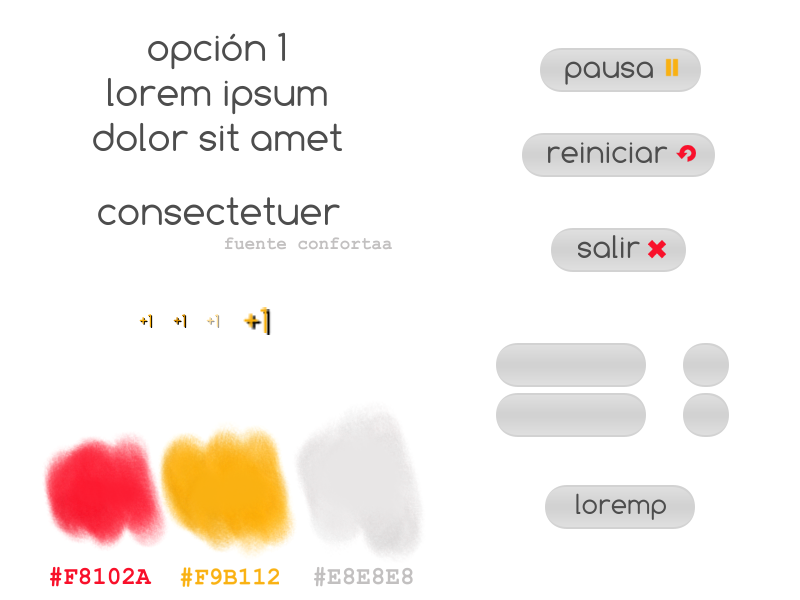
\includegraphics[scale=0.5]{ui.png}
  \end{center}
  \caption{Diferentes elementos utilizados en la interfaz}
\end{figure}

\subsection{Documentación del código}

Por otro lado, para gestionar toda la documentación del proyecto se decidió utilizar las siguientes herramientas:
\begin{itemize}
    \item \LaTeX\ para escribir la memoria, ya que es una forma robusta y fiable de escribir una memoria para
            un Proyecto Fin de Carrera, descartándose otras posibles opciones por no ser adecuadas para la escritura
            de un documento de estas características. Para facilitar la compilación dispone de la herramienta
            GNU Make~\cite{pdf:make}.
    \item Doxygen para la documentación del código fuente, porque además de documentar de manera sencilla y fácil
            de leer el mismo código fuente, genera una documentación en diferentes formatos. Además,
        \begin{itemize}
            \item Doxygen funciona con lenguajes como C++, C, Java, Objective-C, Python, Fortran, VHDL, PHP o C\#
                    (entre otros), por lo que se puede acomodar a nuestras necesidades. Incluso existe una
                    herramienta llamada \textbf{Doxypy} que nos permite reutilizar los comentarios \emph{tipo Python}
                    y adaptarlos a Doxygen, con lo cual ahorramos trabajo y cumplimos con la normativa
                    de código Python.
        \end{itemize}
\end{itemize}

\subsection{Sistema de control de versiones}

El código del proyecto Dominous, está alojado por completo dentro de
la forja que proporciona Rediris, la red española para Interconexión
de los Recursos InformáticoS de las universidades y centros de
investigación, donde tiene su web
oficial~\cite{website:dominous}. Esta forja es básicamente una
instalación de GForge~\cite{website:gforge} con un repositorio
Subversion (SVN) asociado a cada proyecto. \\

Subversion permite llevar un control exahustivo de todos los ficheros e iteraciones de código que se realizan en él,
permitiendo volver a versiones anteriores de código, comprobar diferencias entre versiones o ficheros y cualquier otra
operación propia de un sistema de control de versiones. \\

Se evaluaron otros sistemas de control de versiones distribuidos como GIT, Bazaar o Mercurial, pero se desecharon
básicamente porque, por un lado, este proyecto cuenta únicamente con un desarrollador, y multitud de ventajas que
ofrecen los sistemas de control de versiones distribuidos dejan de tener sentido, si tenemos en cuenta esta circunstancia
del proyecto, y por otro lado la integración de SVN con Rediris (con las ventajas de visualización de código y versiones
que ofrece ViewCVS) decantaron la decisión sobre el lado de SVN.

\section{Interfaz gráfica}

Tomando los resultados obtenidos en la fase de análisis es necesario diseñar una interfaz gráfica amigable
para el usuario y desde la cual se pueda interactuar con la aplicación. Para el diseño de las interfaces
se intentará en todo momento que sean usables además de intentar conseguir que el usuario no pueda
introducir datos erróneas para que no produzca comportamientos anómalos. \\

\begin{figure}[h]
  \label{fig:pantallas_interfaz}
  \begin{center}
    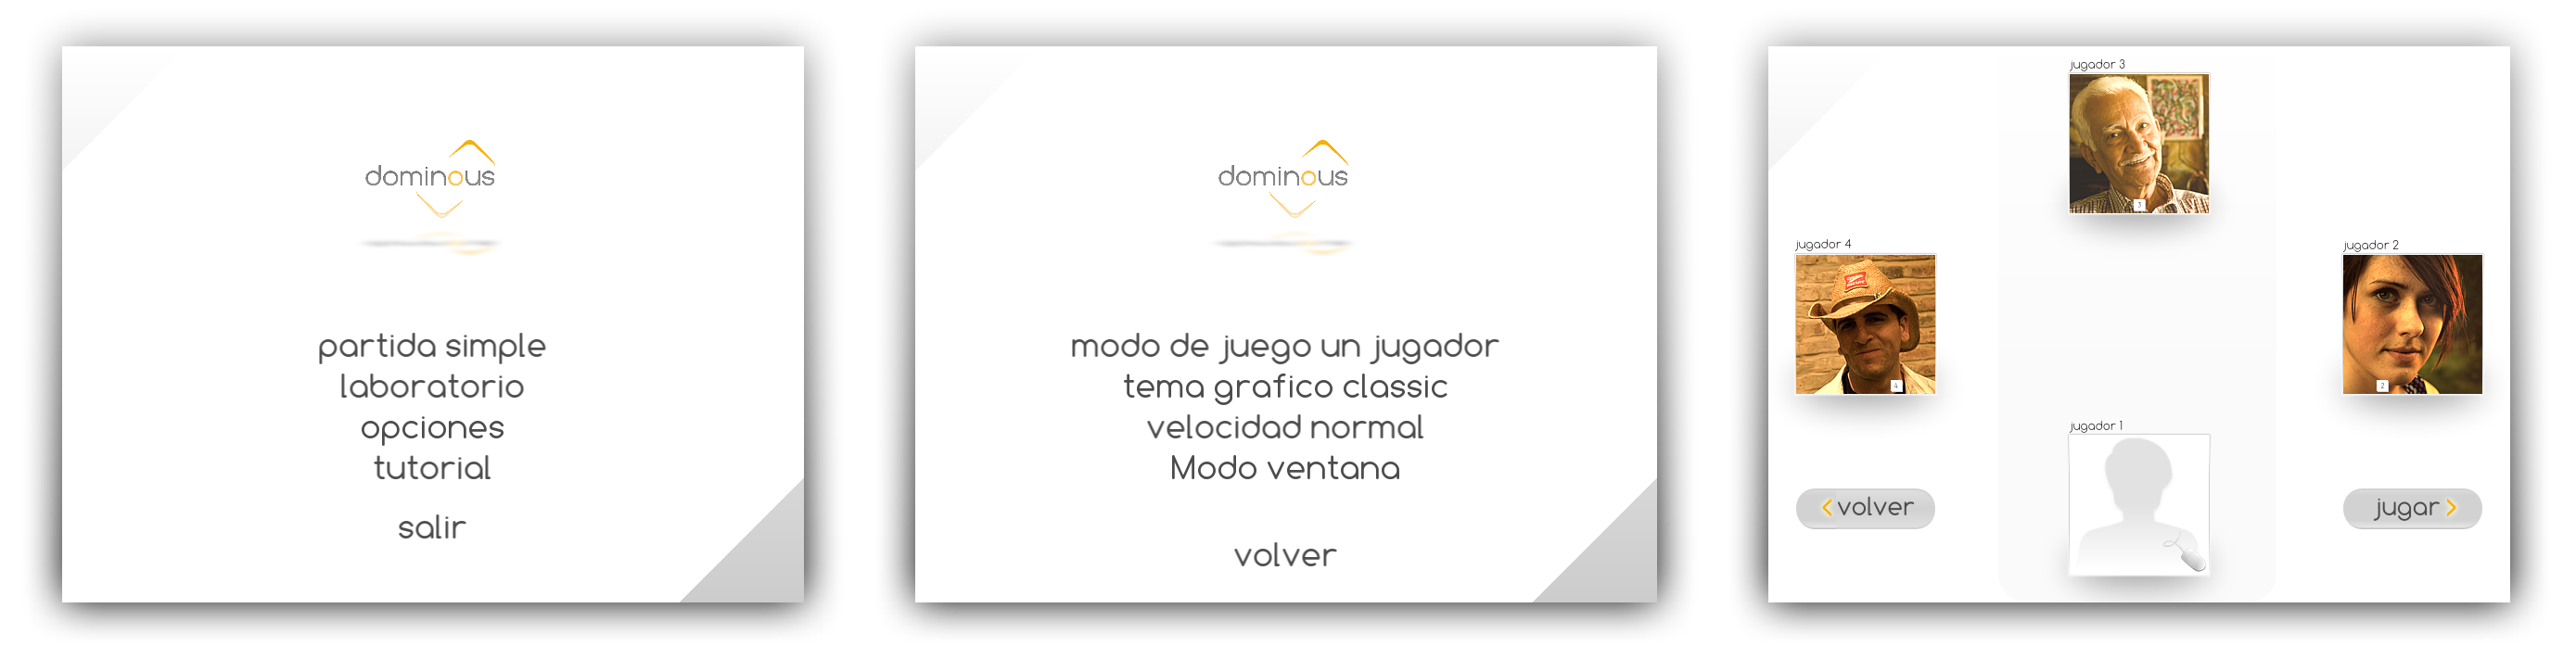
\includegraphics[scale=0.25]{interfaz.png}
  \end{center}
  \caption{Varias pantallas con la interfaz de Dominous}
\end{figure}

\subsection{Diagrama de interacción entre interfaces gráficas}

En el siguiente diagrama~\ref{fig:diagramainteraccioninterfaces} podemos observar la interacción entre
las distintas interfaces gráficas desarrolladas para la aplicación. \\

\begin{figure}[h]
  \label{fig:diagramainteraccioninterfaces}
  \begin{center}
    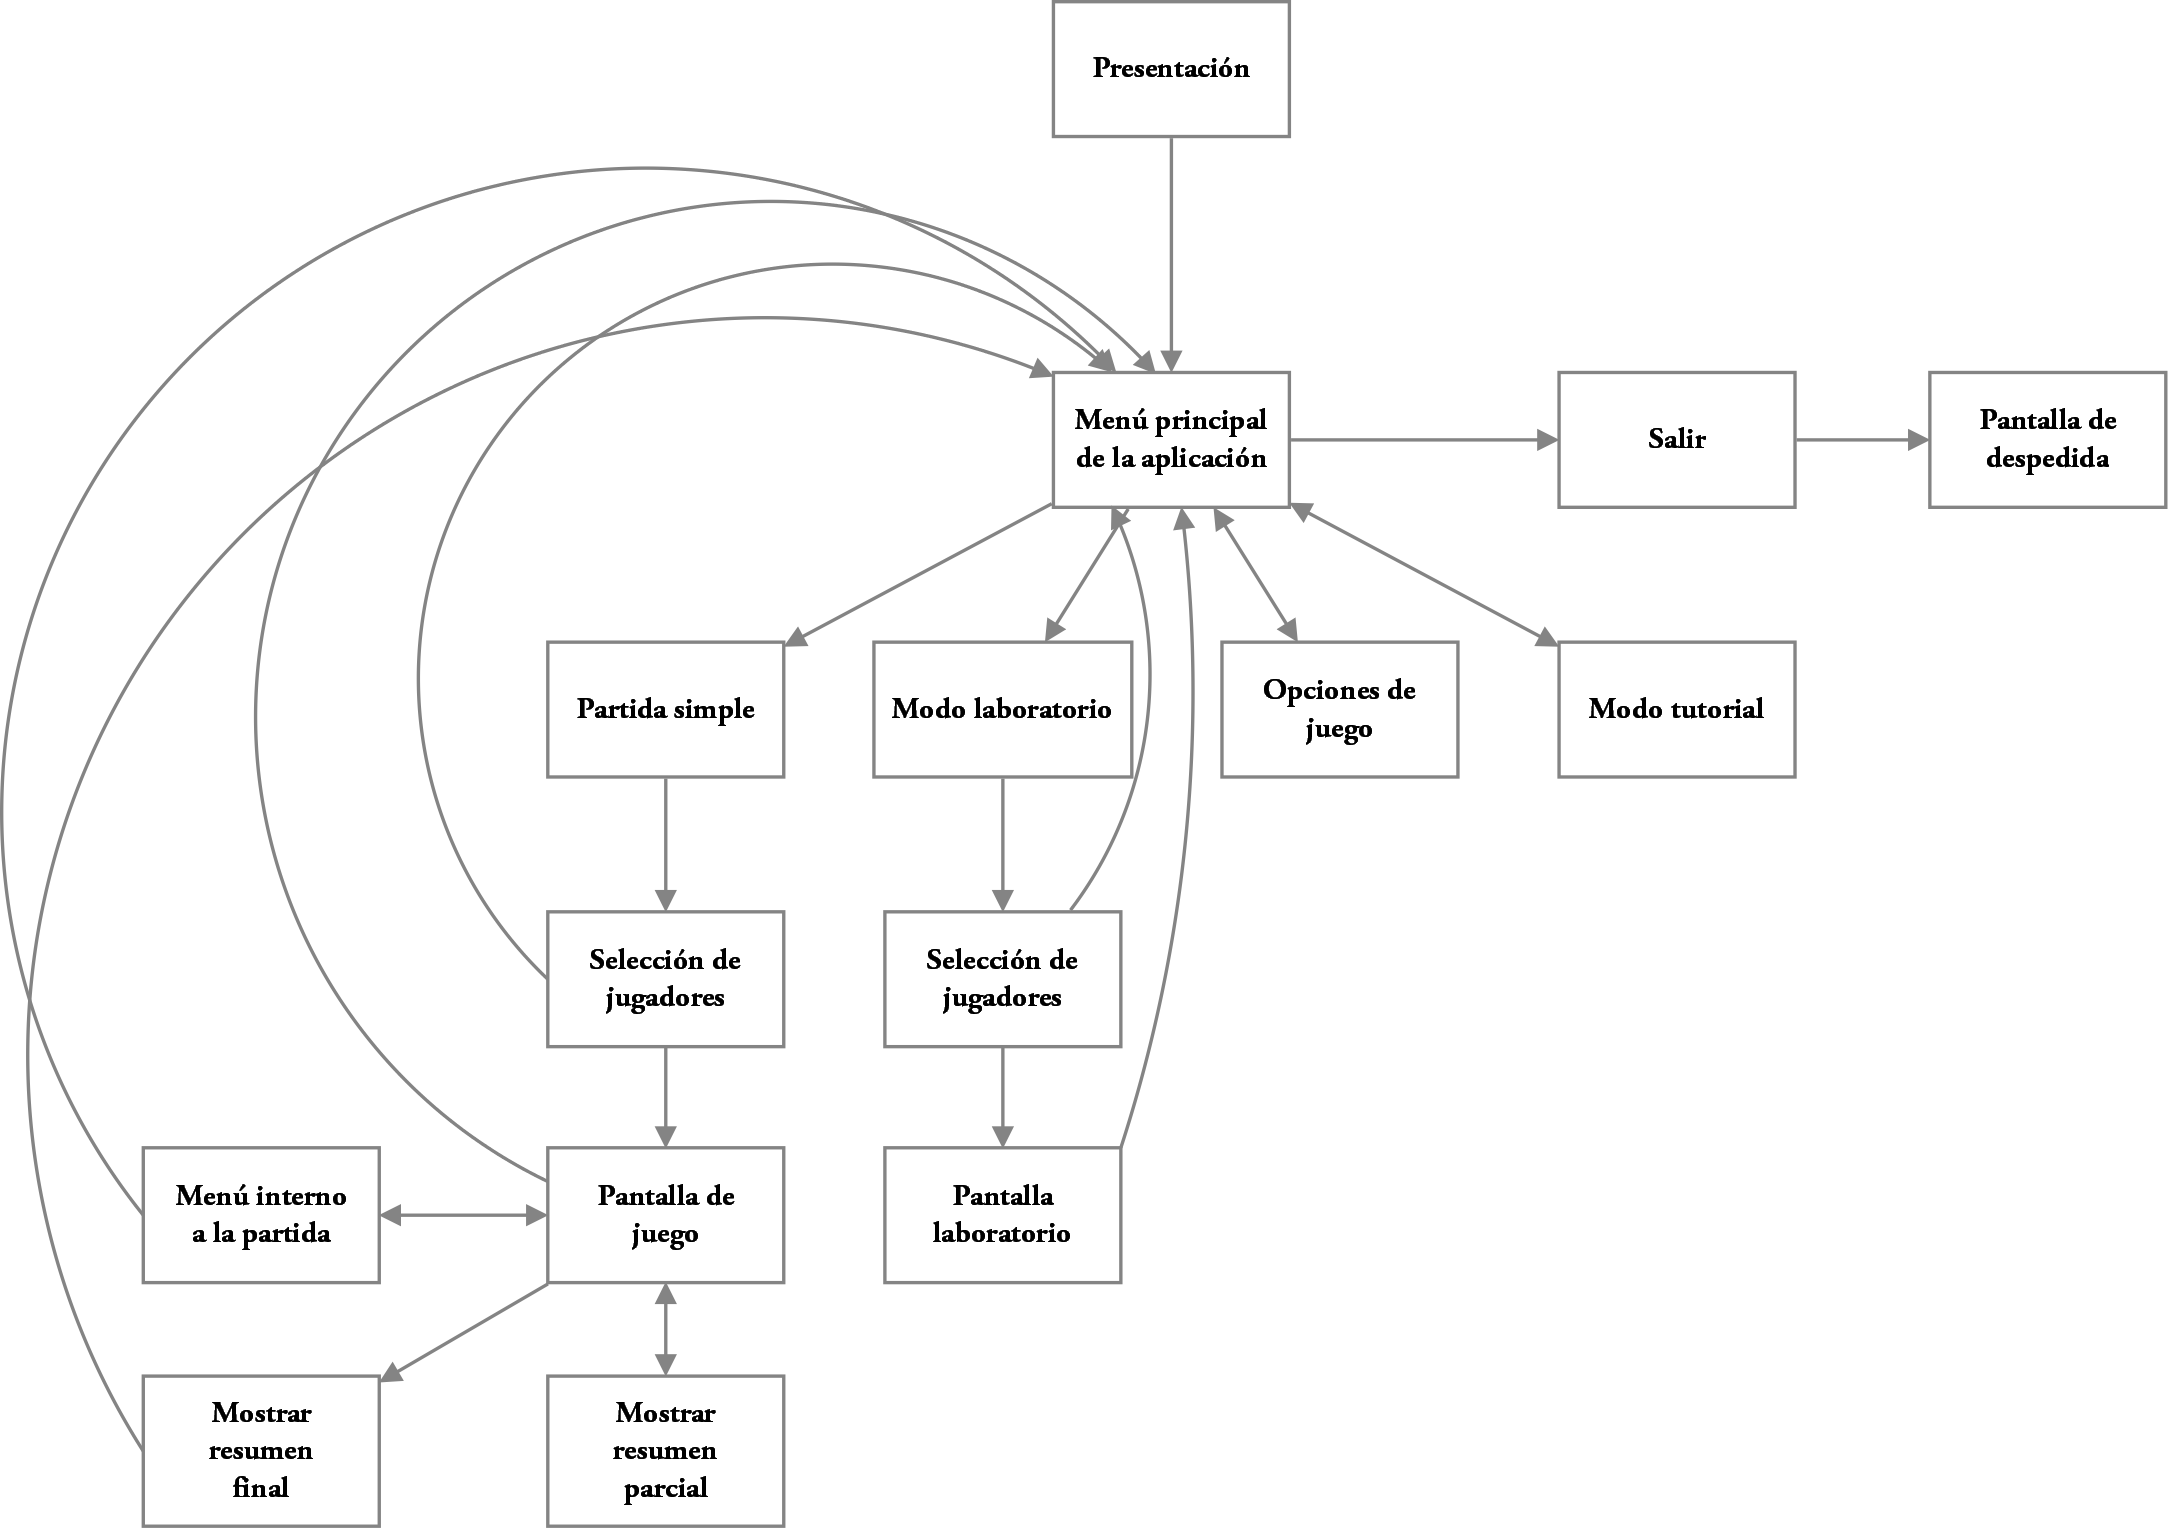
\includegraphics[scale=0.15]{diagrama_interfaces.png}
  \end{center}
  \caption{Diagrama de interacción entre interfaces}
\end{figure}

\section{Diagrama Entidad -- Relación}

La aplicación \textbf{Dominous} realiza un almacenamiento limitado de información, por lo que no se estima necesario
realizar un diagrama Entidad -- Relación con este fin.

\section{Diagrama de clases de diseño}

A continuación se muestra el diagrama de clases de diseño para \textbf{Dominous} (figura~\vref{fig:diagrama_clases_diseno}).

\begin{figure}[h]
  \label{fig:diagrama_clases_diseno}
  \begin{center}
%    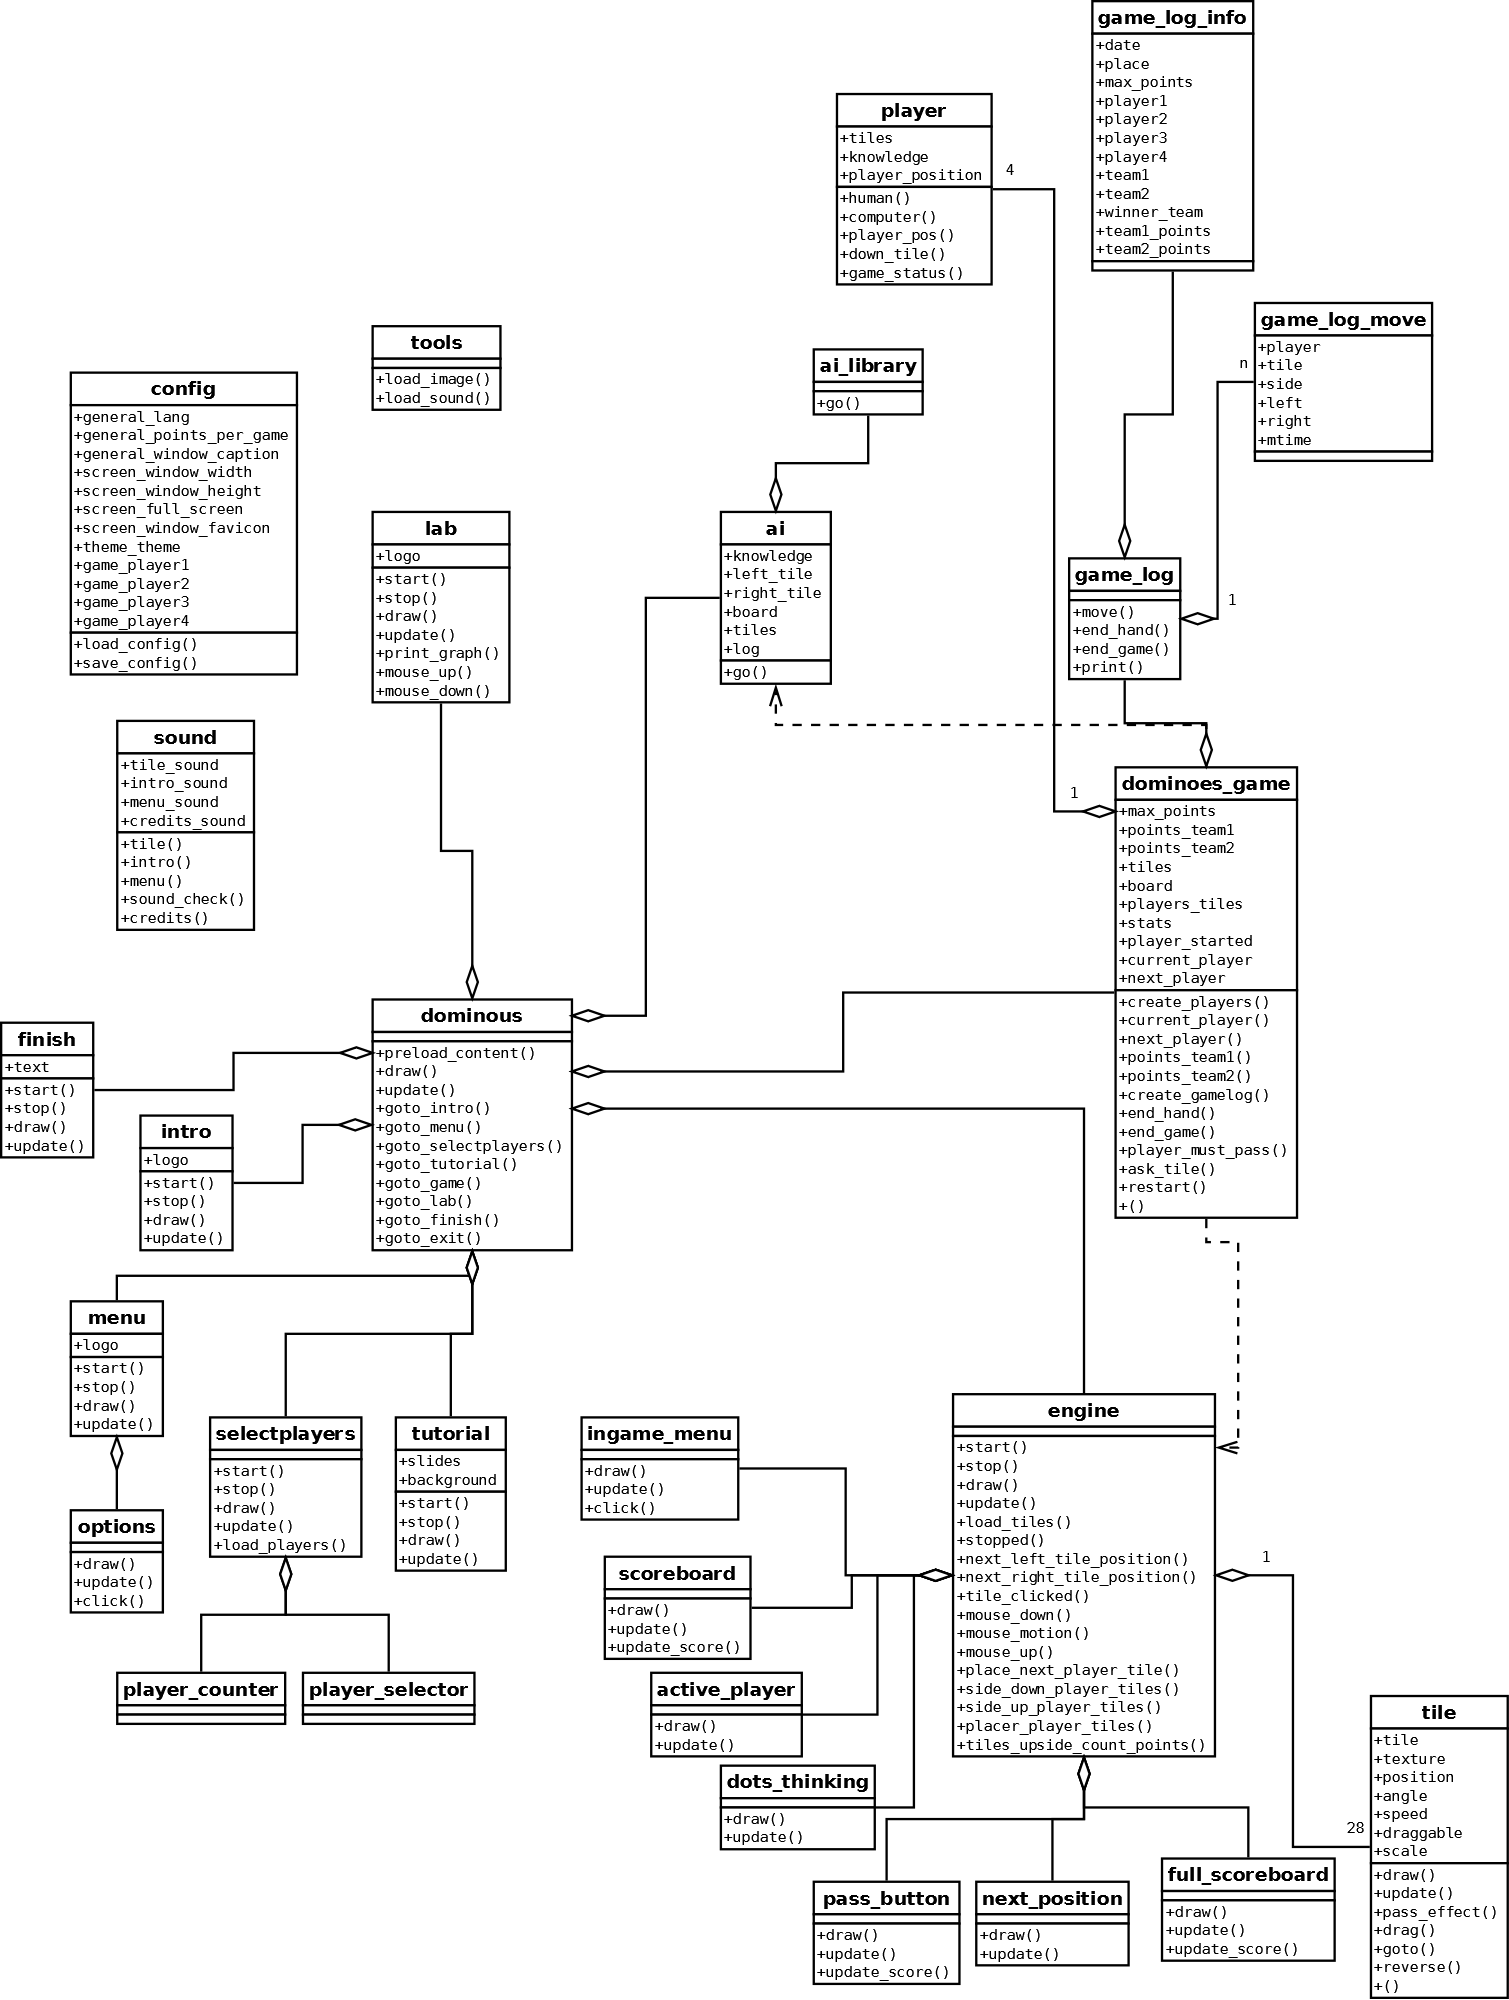
\includegraphics[scale=0.23]{diagrama_clases_diseno.png}
%    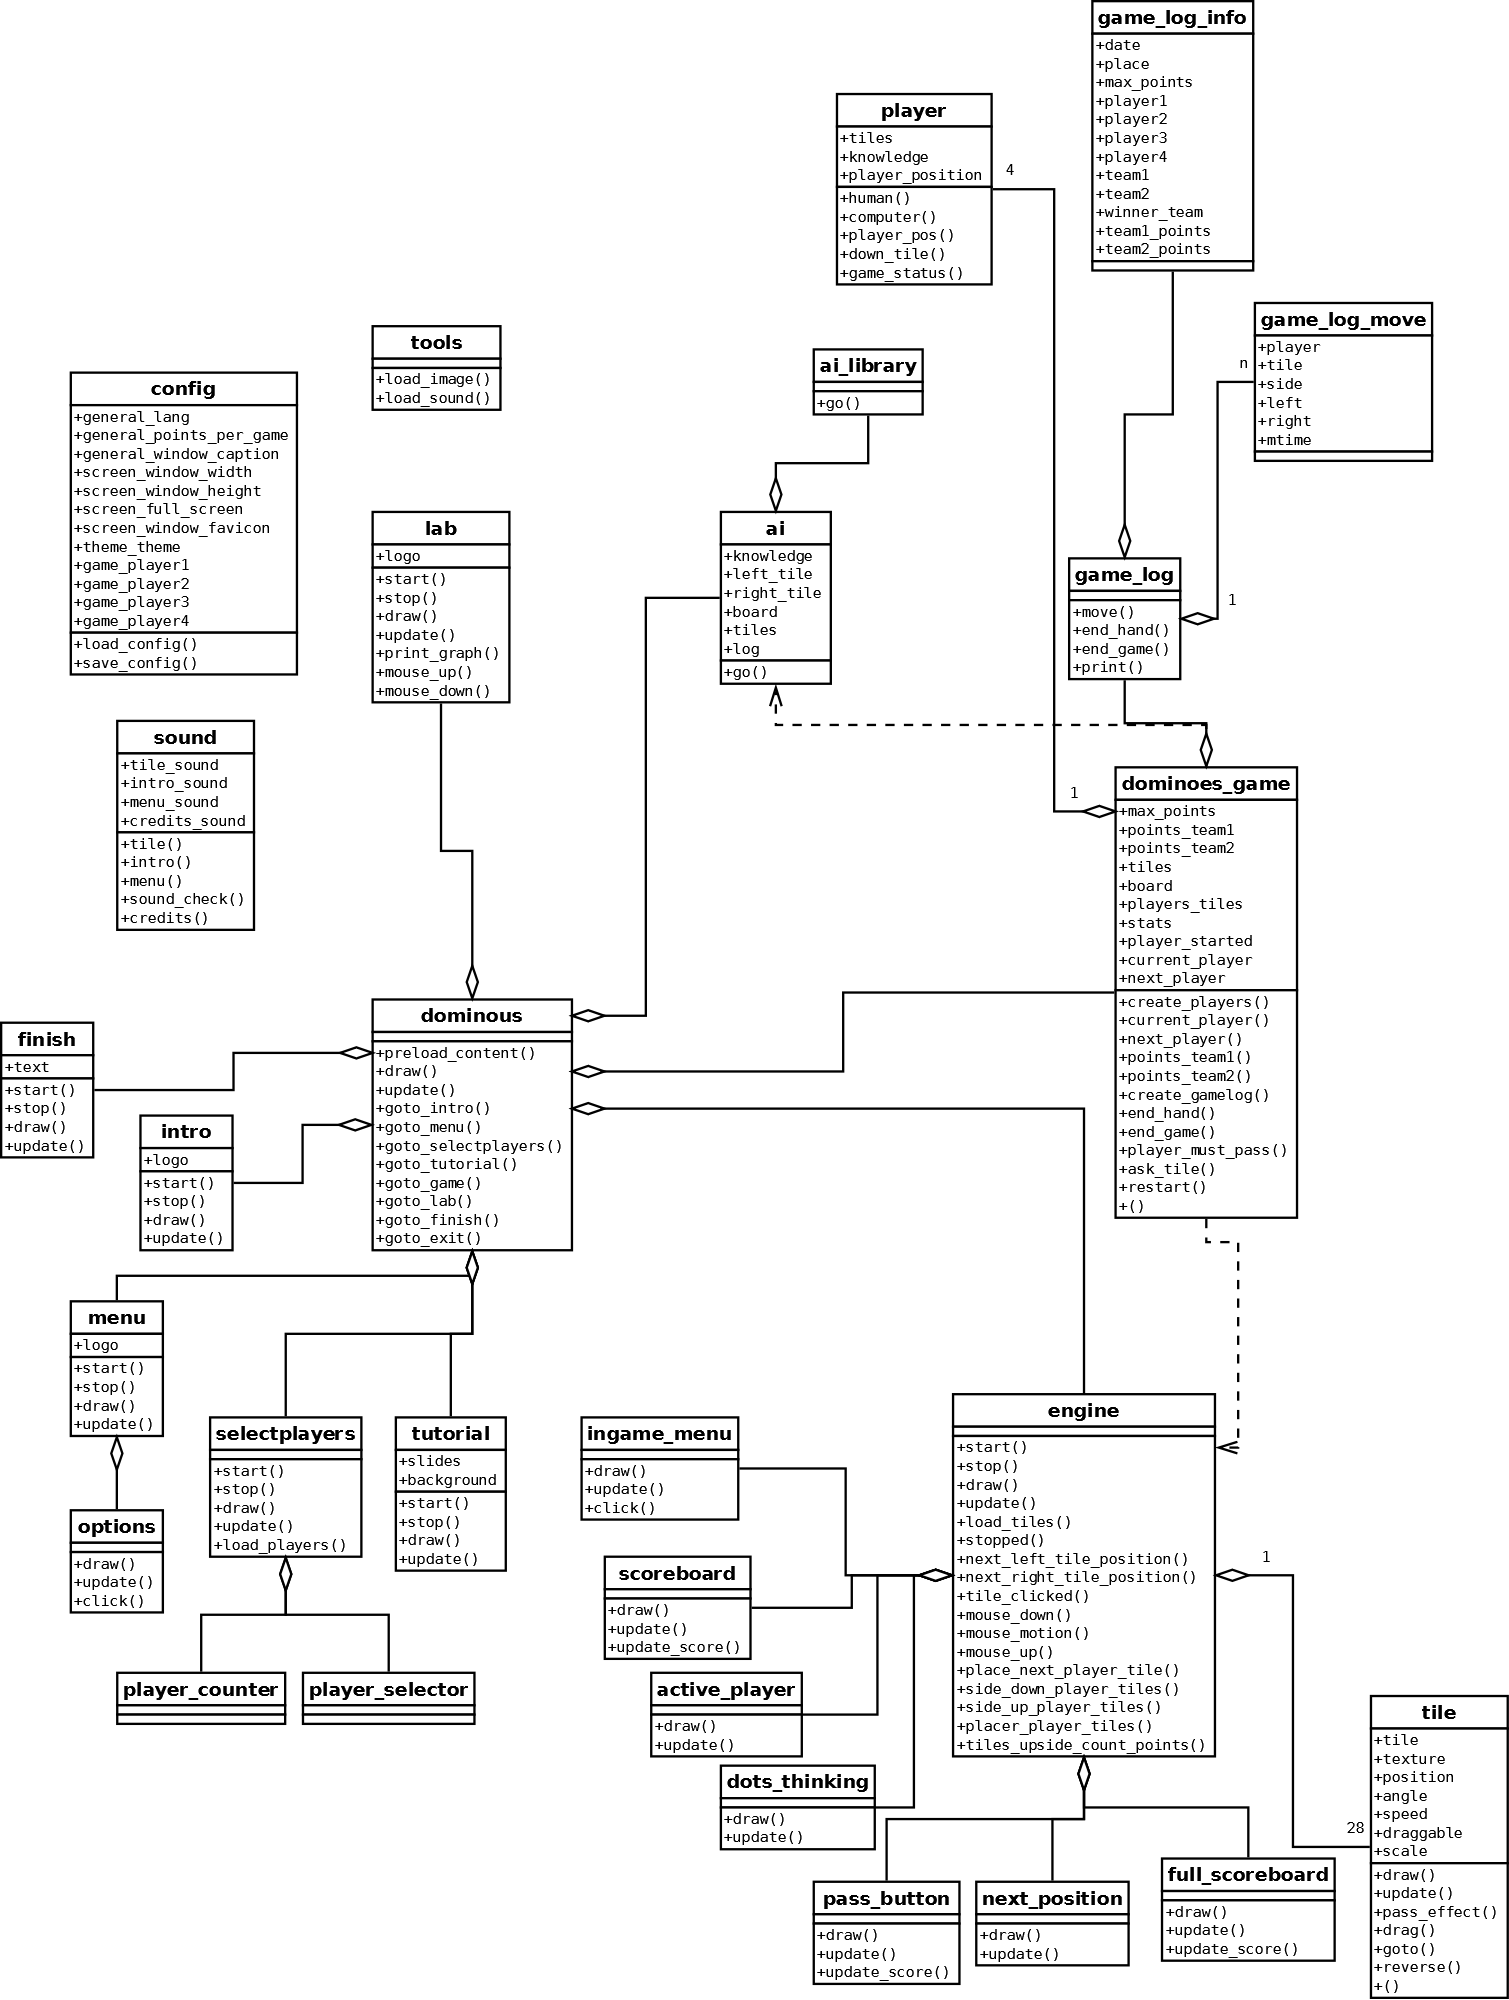
\includegraphics[width=0.9\textwidth]{diagrama_clases_diseno.png}
    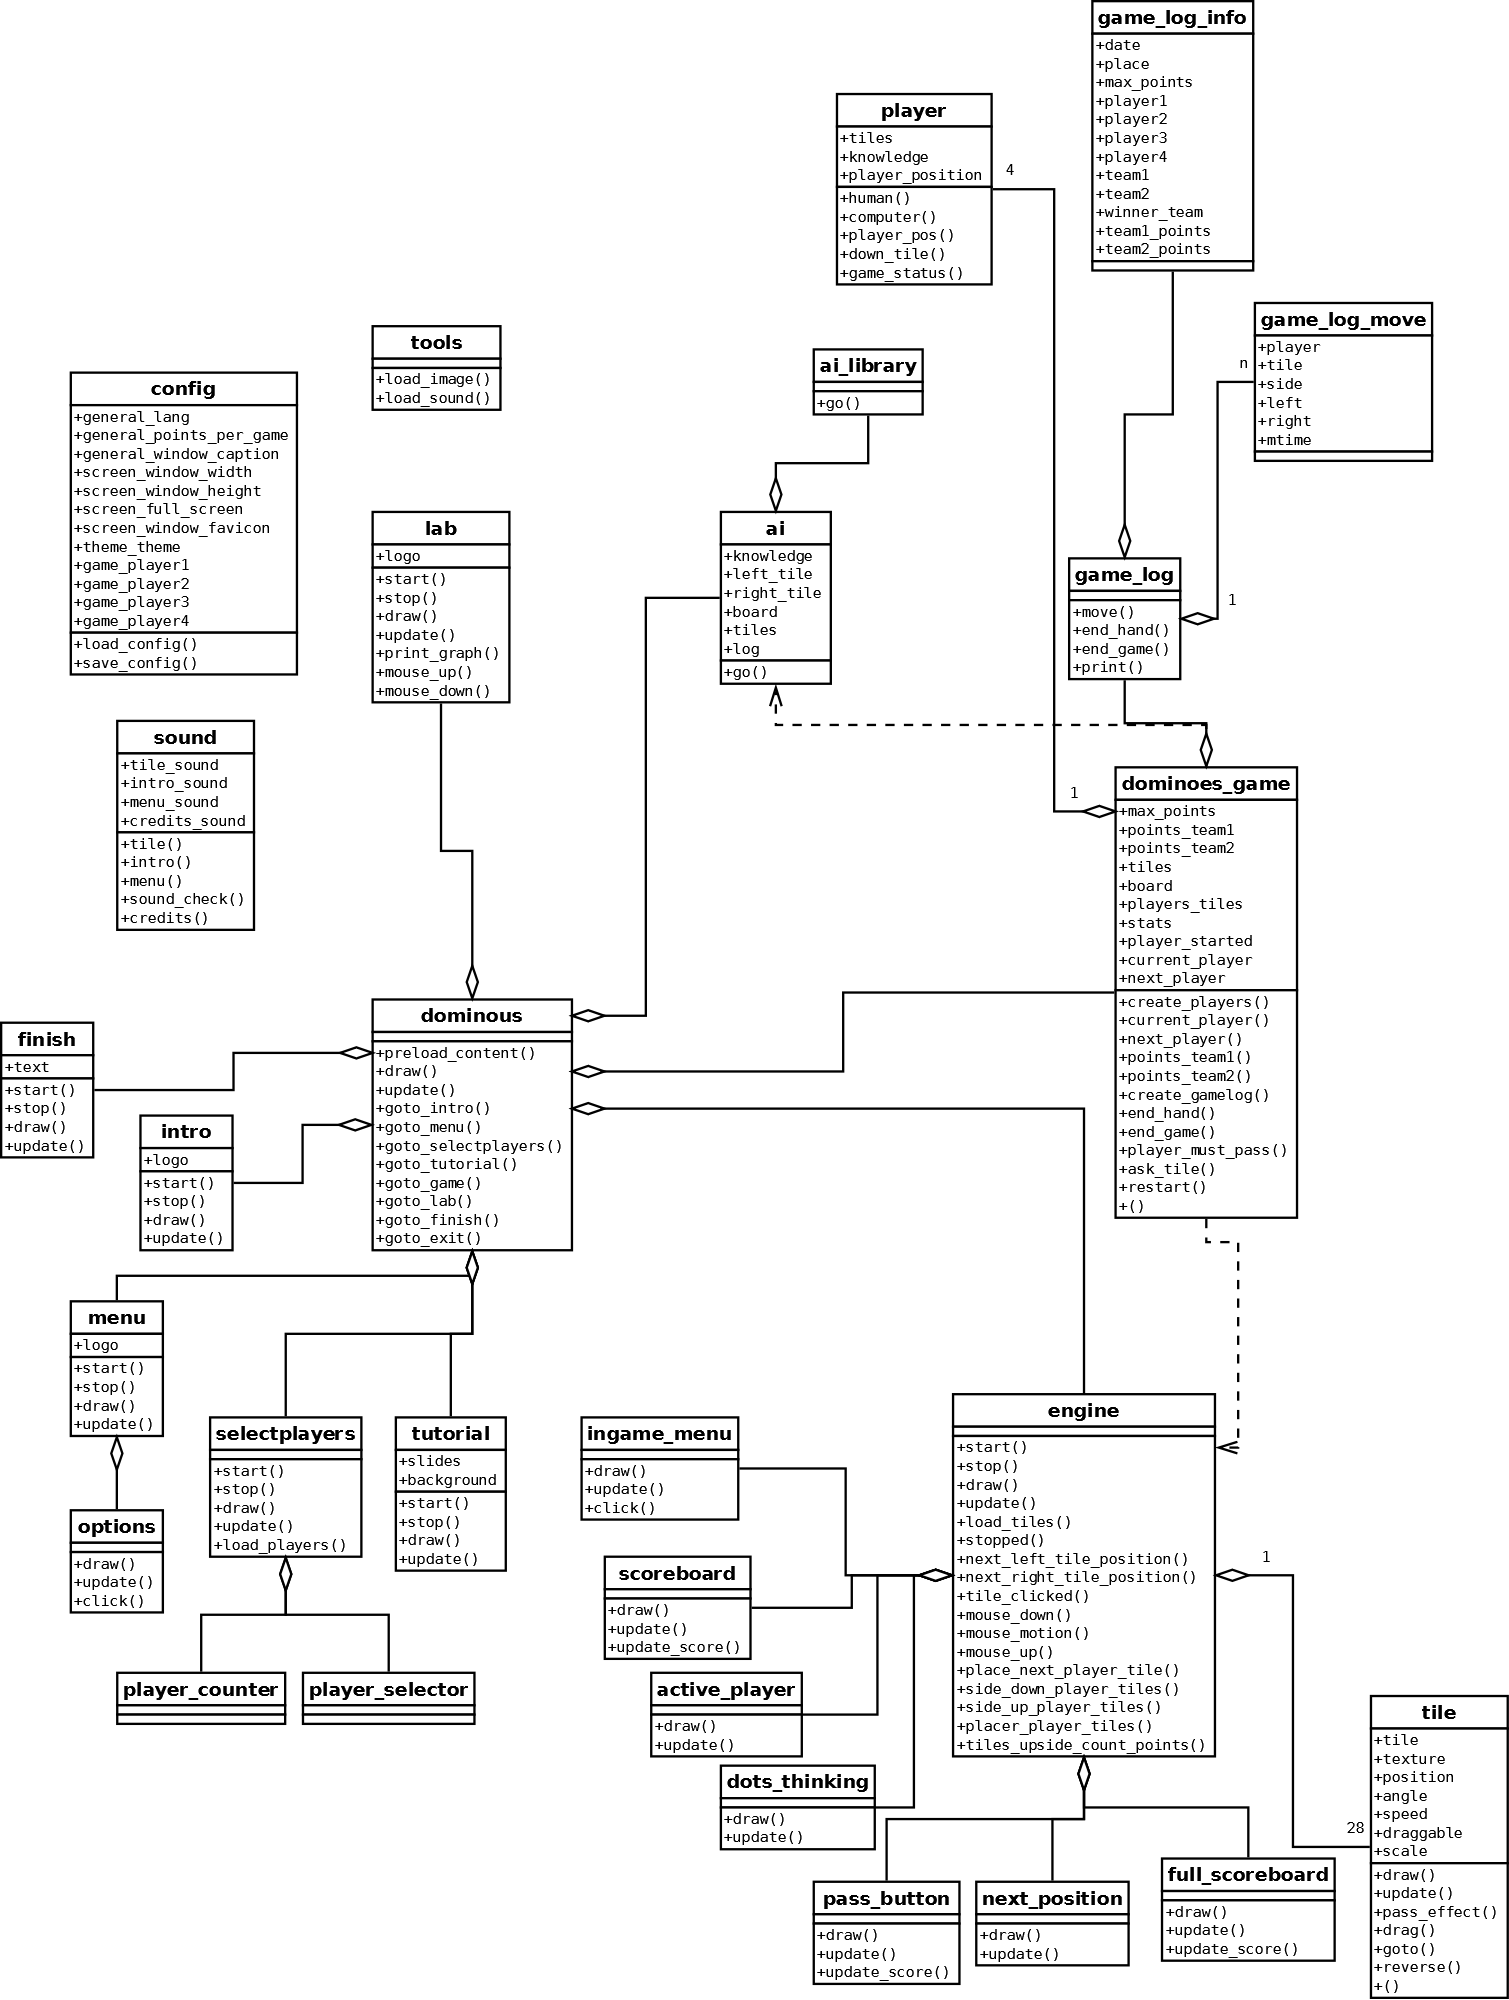
\includegraphics[width=1\textwidth]{diagrama_clases_diseno.png}
  \end{center}
  \caption{Diagrama de diseño del sistema}
\end{figure}


\section{Análisis de las principales clases de la aplicación}

En este apartado realizaremos un repaso a las principales clases que intervienen en el diseño de \textbf{Dominous},
definiendo los métodos y atributos que se requieren para el correcto desarrollo de la aplicación y comentando
todos los apartados cuya funcionalidad merezca ser destacada.

\subsection{Clase dominous}

La clase dominous genera el objeto principal que soporta el peso principal de toda la aplicación. Al inicio de la
ejecución se crea un objeto de esta clase; este objeto va creando --- según las necesidades del flujo que tome
la ejecución de la misma --- los diferentes objetos, controlando y dando paso a la interfaz activa, llamando a
las principales funciones y permitiendo la captura de los eventos de entrada. \\

Al igual que la gran mayoría de videojuegos, para el desarrollo de Dominous se han utilizado dos métodos principales
que permiten controlar la aplicación en tiempo real. Estos dos métodos son:
\begin{description}
    \item[draw] El primer método se encarga de dibujar en pantalla todos los elementos de la interfaz. El funcionamiento
        básico es recorrer todos los objetos activos y pintarlos según la posición, rotación y escala que tengan en
        ese preciso momento. 
    \item[update] El segundo método se ocupa de realizar los cálculos para el movimiento de los elementos gráficos. 
        En cada iteración cambiará el estado de los objetos activos, modificando la imagen o los valores posición,
        rotación y/o escala, estudiando las posibles colisiones, eventos y cualquier otra circunstancia que cambie
        el estado de la aplicación, para que en el siguiente ciclo se dibujen los elementos en su posición correcta.
\end{description}

Una vez que este objeto principal toma el control de la aplicación, su función es llamar a los métodos \comando{draw}
y \comando{update} del objeto encargado de la interfaz que estemos mostrando actualmente, de forma alternativa. \\

Este juego de llamadas a ambos métodos se realizará hasta un máximo de 60 veces por segundo, dependiendo del rendimiento
que se obtenga de los recursos del sistema. De esta forma conseguiremos un máximo de 60 frames o cuadros por segundo,
que serán los encargados de generar la sensación de movimiento. \\

Como vemos, el objeto de la clase dominous no realiza ningún dibujado en pantalla ni cálculos, sino que su único
cometido es redireccionar el flujo de la aplicación al objeto correspondiente.

\subsection{Clase dominoes\_game}

La labor de esta clase es llevar el control de una partida completa de dominó, siguiendo las reglas del \textbf{dominó
internacional}. Dependiendo de la configuración de la partida, creará los jugadores según la selección que se haya
realizado en la pantalla de selección de personajes y comenzará con el bucle principal: \\

Repartirá las fichas entre los diferentes participantes del juego e irá pidiendo fichas a los jugadores de forma
consecutiva, hasta que se de alguna circunstancia de finalización de la mano. \\

Este bucle se repetirá hasta que alguno de los dos equipos alcance o supere los 200 puntos, momento en el cual la partida
se dará por finalizada. \\

Esta clase también mantendrá activo y actualizado un fichero de log con toda la información generada en la partida. Esta
información se utilizará más tarde en el apartado de inteligencia artificial, y almacenará los datos utilizando
la siguiente estructura: \\

Por un lado tenemos la información global de la partida: 

\begin{description}
    \item[date] Fecha de desarrollo de la partida.
    \item[place] Lugar donde tuvo lugar la partida.
    \item[max\_points] Límite superior de puntos necesarios para ganar el encuentro. Como se utilizan las reglas del
        \textbf{dominó internacional}, esta cota estará situada en los doscientos puntos.
    \item[player1] Datos del jugador 1.
    \item[player2] Datos del jugador 2.
    \item[player3] Datos del jugador 3.
    \item[player4] Datos del jugador 4.
    \item[team1] Pareja que forma el equipo 1.
    \item[team2] Pareja que forma el equipo 2.
    \item[points\_team1] Puntos actuales que tiene el equipo 1.
    \item[points\_team2] Puntos actuales que tiene el equipo 2.
    \item[winner\_team] Pareja que finalmente ha sido ganadora de la partida.
\end{description}

Y por otro lado tenemos información relativa a la mano que se está desarrollando actualmente. Esta información se repite
por cada movimiento que se realice en la partida, y se agrupa por manos:

\begin{description}
    \item[player] Jugador que ha realizado el movimiento.
    \item[tile] Ficha que ha colocado.
    \item[side] Lado del tablero por donde ha colocado la ficha.
    \item[left] Cifra, del cero al siete, que se tiene como resultante del movimiento por el lado izquierdo del tablero.
    \item[right] Cifra, del cero al siete, que se tiene como resultante del movimiento por el lado derecho del tablero.
    \item[mtime] Tiempo (en segundos) que ha estado pensando el jugador antes de colocar la ficha.
\end{description}


\section{Sistemas expertos}

En este apartado de la memoria requiere de una especial explicación, ya que a la hora de realizar un videojuego de
dominó goza de gran importancia los diferentes sistemas expertos que participarán en la partida. Estos sistemas expertos,
como bien su nombre indica, simulan el comportamiento de un ser humano experto en una materia, en este caso del juego
de dominó, y su realismo debe hacer sentir al jugador humano que está desempeñando una partida real contra jugadores
también humanos. \\

Enfrentarse a una simulación de inteligencia artificial es una de las empresas más difíciles y complicadas pero a la
vez placenteras y satisfactorias de abarcar en un proyecto de Ingeniería del Software. Los seres humanos utilizan
multitud de métodos y herramientas para razonar y obtener soluciones a problemas concretos, y en muchas ocasiones
este tipo de comportamientos son imposibles de simular, bien por la complejidad computacional que supone, bien por
desconocimiento del funcionamiento exacto que sigue el cerebro para obtener esa solución, o bien por limitaciones de
recursos, ya sea de disco, tiempo de desarrollo o metodologías que simulen ese comportamiento. \\

Por otro lado, aunque el público neófito en la materia pueda suponer que el dominó es un juego de suerte, con un
abanico muy corto de opciones de juego o con una libertad de movimientos muy limitada, nada más lejos de la realidad. \\

El dominó es un juego muy profundo, con normas, técnicas y muchas dosis de psicología, un deporte que obliga al
jugador a estar concentrado al cien por cien durante todo el desarrollo del juego, y un arte con una curva de
aprendizaje poco escarpada, que permite que jugadores nóveles puedan adentrarse en el juego, pero que presenta
mucha complicación convertirse en un gran jugador de dominó. \\

Y, si estas razones que explican la complejidad del mismo no fueran suficientes, no hay más que echarle un vistazo
a los torneos locales o de ámbitos más abiertos para descubrir que las parejas de grandes jugadores sabios y con
una gran compenetración son los que suelen ganar, descartando de forma tajante la posibilidad de que sea la suerte
la que empuje la balanza de la partida hacia un equipo u otro. \\

A la hora de afrontar este problema, el primer paso fue empaparse de cultura y conocimiento sobre el dominó. Las
principales herramientas que se utilizaron fueron:

\begin{description}
    \item[El Libro del dominó] de Benito Ruipérez \cite{mora90}, un libro ameno y profundo sobre el mundo del dominó,
        con multitud de partidas explicadas movimiento a movimiento, trucos, ejemplos, técnicas básicas y avanzadas y
        mucha información.
    \item[Don Manuel Palomo Fernández de Bobadilla] -- jugador amateur de dominó y participante en torneos durante más de cuarenta
        años, con un gran conocimiento de técnicas y métodos de juego, mucha experiencia y una gran facilidad para
        comunicar toda esa sabiduría y conocimiento.
\end{description}

Después de profundizar en el mundo del dominó, y tener cierto conocimiento sobre el mismo --- aunque nada comparado
con el que pueden tener jugadores más experimentados de este juego --- podemos intentar definir las pautas sobre
las que va a llevarse a cabo la simulación del sistema experto de dominó. \\

Lo primero que observamos es que la estrategia que siga cada jugador depende enteramente del rol que desempeñe el mismo.
Como vimos en el capítulo ~\ref{juegoporparejas} es importante definir una estrategia personalizada para cada jugador,
dependiendo del lugar respecto al jugador mano.

\subsection{Modelado}

Tras realizar un análisis del sistema, se han identificado los siguientes hechos necesarios para que el sistema experto razone:

\begin{description}
\item[Ficha]
\item[Turno]
\item[Jugador que manda]
\end{description}

En cuanto al motor de inferencia se ha implementado un sencillo motor basado en prioridades de las reglas.




\chapter{Implementación}
% -*-cap2.tex-*-
% Este fichero es parte de la plantilla LaTeX para
% la realización de Proyectos Final de Carrera, protegido
% bajo los términos de la licencia GFDL.
% Para más información, la licencia completa viene incluida en el
% fichero fdl-1.3.tex

% Copyright (C) 2009 Pablo Recio Quijano 

\section{Implementación}

Una vez terminadas las dos fases previas --- análisis y diseño --- es hora de enfrentarnos a la codificación e implementación
en sí de la aplicación. Este apartado es largo y entretenido, y va descubriendo a cada momento nuevas problemáticas que
no se han tenido en cuenta antes y es necesario resolver, pero también es apasionante, porque vamos viendo de forma
empírica cómo nuestra aplicación va tomando forma y se va haciendo tangible a cada momento que avanza. \\

El desarrollo de Dominous ha presentado muchas características interesantes, problemas, dificultades y otras circunstancias
que creemos interesante destacar, y que se pasamos a comentar a continuación.

\subsection{Entorno gráfico}

El entorno gráfico se puede dividir en dos apartados de diferente complejidad: por un lado tenemos la gestión de menús,
opciones, pantallas y secciones de la aplicación, y por otro lado tenemos la gestión de una partida de dominó, con todas
sus interacciones, animaciones y movimientos de fichas, eventos y demás.

\subsubsection{Sistema de secciones}

Todo el sistema de secciones lo gobierna el objeto principal de la aplicación, llamado \textbf{dominous}. Este objeto posee
diferentes objetos como atributos, y estos atributos son las diferentes secciones de la aplicación. Cuando queremos
que el flujo de la aplicación pase de una sección a otra no tenemos más que llamarla; al llamarla estaremos ejecutando
el siguiente fragmento:

\begin{lstlisting} [caption={Código Python de cambio de sección}, language=Python, numbers=left]
def goto_tutorial(self):
    self.flow.stop()
    self.flow = self.tutorial
    self.flow.start()
\end{lstlisting}

Gracias a este tipo de llamadas podemos subdividir cómodamente la aplicación en módulos muy acotados, a los cuales se aplica
primero una función de inicialización --- por si es necesario que actualicen estructuras, datos o cualquier otra labor
de preparación que puedan requerir --- y una vez se termina también se ejecuta una función de finalización. \\

Y mientras el flujo esté asociado a una sección, todas las funciones de eventos, dibujado y actualización de la pantalla
se disparan dentro de la sección correspondiente. \\

Gracias a esta metodología hemos podido acotar de forma muy cómoda las diferentes secciones (cada una con sus peculiaridades)
y gestionar de forma independiente cada apartado, evitando posibles problemas colaterales, asegurando una buena
integración y minimizando el hecho de que errores de un apartado puedan afectar a otros.

\subsubsection{Gestión de partida}

La gestión de la partida se puede dividir en dos apartados principales. El primero de ellos es la gestión de los diferentes
estados y transiciones en los que se divide la partida, y el segundo es el motor gráfico en sí, que dibuja y mueve
las fichas, el tablero y todos los diferentes elementos interactivos que incluye el juego. \\

La gestión de estados se ha programado con una máquina finita de estados --- o autómata finito --- ya que este tipo de
juegos por turnos se controla de forma cómoda y fácil con este tipo de estructuras. Contamos con un atributo \textbf{status}
de la clase principal; este estado se va comprobando y actualizando en los diferentes estados, tal y como se ve en la
estructura siguiente:

\begin{lstlisting} [caption={Autómata finito de estados}, language=Python, numbers=left]
"""
Status = 0 - game start, reset all, create players
    1 - fade in
    2 - deal tiles
    if game is over:
        999 - end game, goto menu
    if hand is over:
        99 - end hand
        100 - move tiles to center
        101 - show full screen scoreboard
        goto 1
    else:
        3 - draw available positions
        4 - ask tile next player
        if next player is human:
            if player must pass:
                20 - human player must pass
                21 - waiting to click pass button
                22 - human pressed pass button
                23 - pass effect
                goto 5
            else:
                6 - start drag n drop player tile
                7 - dragging tile
                8 - mousedown released
                if player can place tile here:
                    goto 5
                else:
                    goto 6
        else:
            if computer must pass:
                23 - pass effect
            else:
                5 - move tile to its place
            goto 3
"""
\end{lstlisting}

Así, siguiendo este diagrama de flujo con las posibles transiciones entre los diferentes estados, podemos definir y acotar
los posibles movimientos que se llevan a cabo a lo largo de la partida. \\

Por otro lado, el motor gráfico que participa de la partida consta de varios apartados y, probablemente, uno de los más costosos y
laboriosos fue el del método que decide en qué lugar se coloca una ficha en el tablero. \\

Como vemos en el gráfico~\ref{fig:tiles-position} existen multitud de posiciones y orientaciones posibles a la hora de colocar
la nueva ficha --- hasta un total de 20 diferentes posiciones, dependiendo de las siguientes variables:
\begin{itemize}
    \item Naturaleza de la ficha que vamos a colocar --- recordemos que las fichas dobles se colocan de forma
            perpendicular al sentido del flujo de las fichas, mientras que las fichas que no son dobles continúan con
            el sentido de las fichas.
    \item Orientación de la ficha de enganche.
    \item Sentido de las fichas en el tablero.
    \item Posición de la ficha de enganche en el tablero respecto a los límites del mismo.
    \item Número de fichas colocadas en el tablero --- si estamos colocando la primera ficha, ésta debe situarse en
            el centro justo del tablero.
    \item Tamaño de las fichas y del área de juego.
\end{itemize}

\begin{figure}[h]
  \begin{center}
    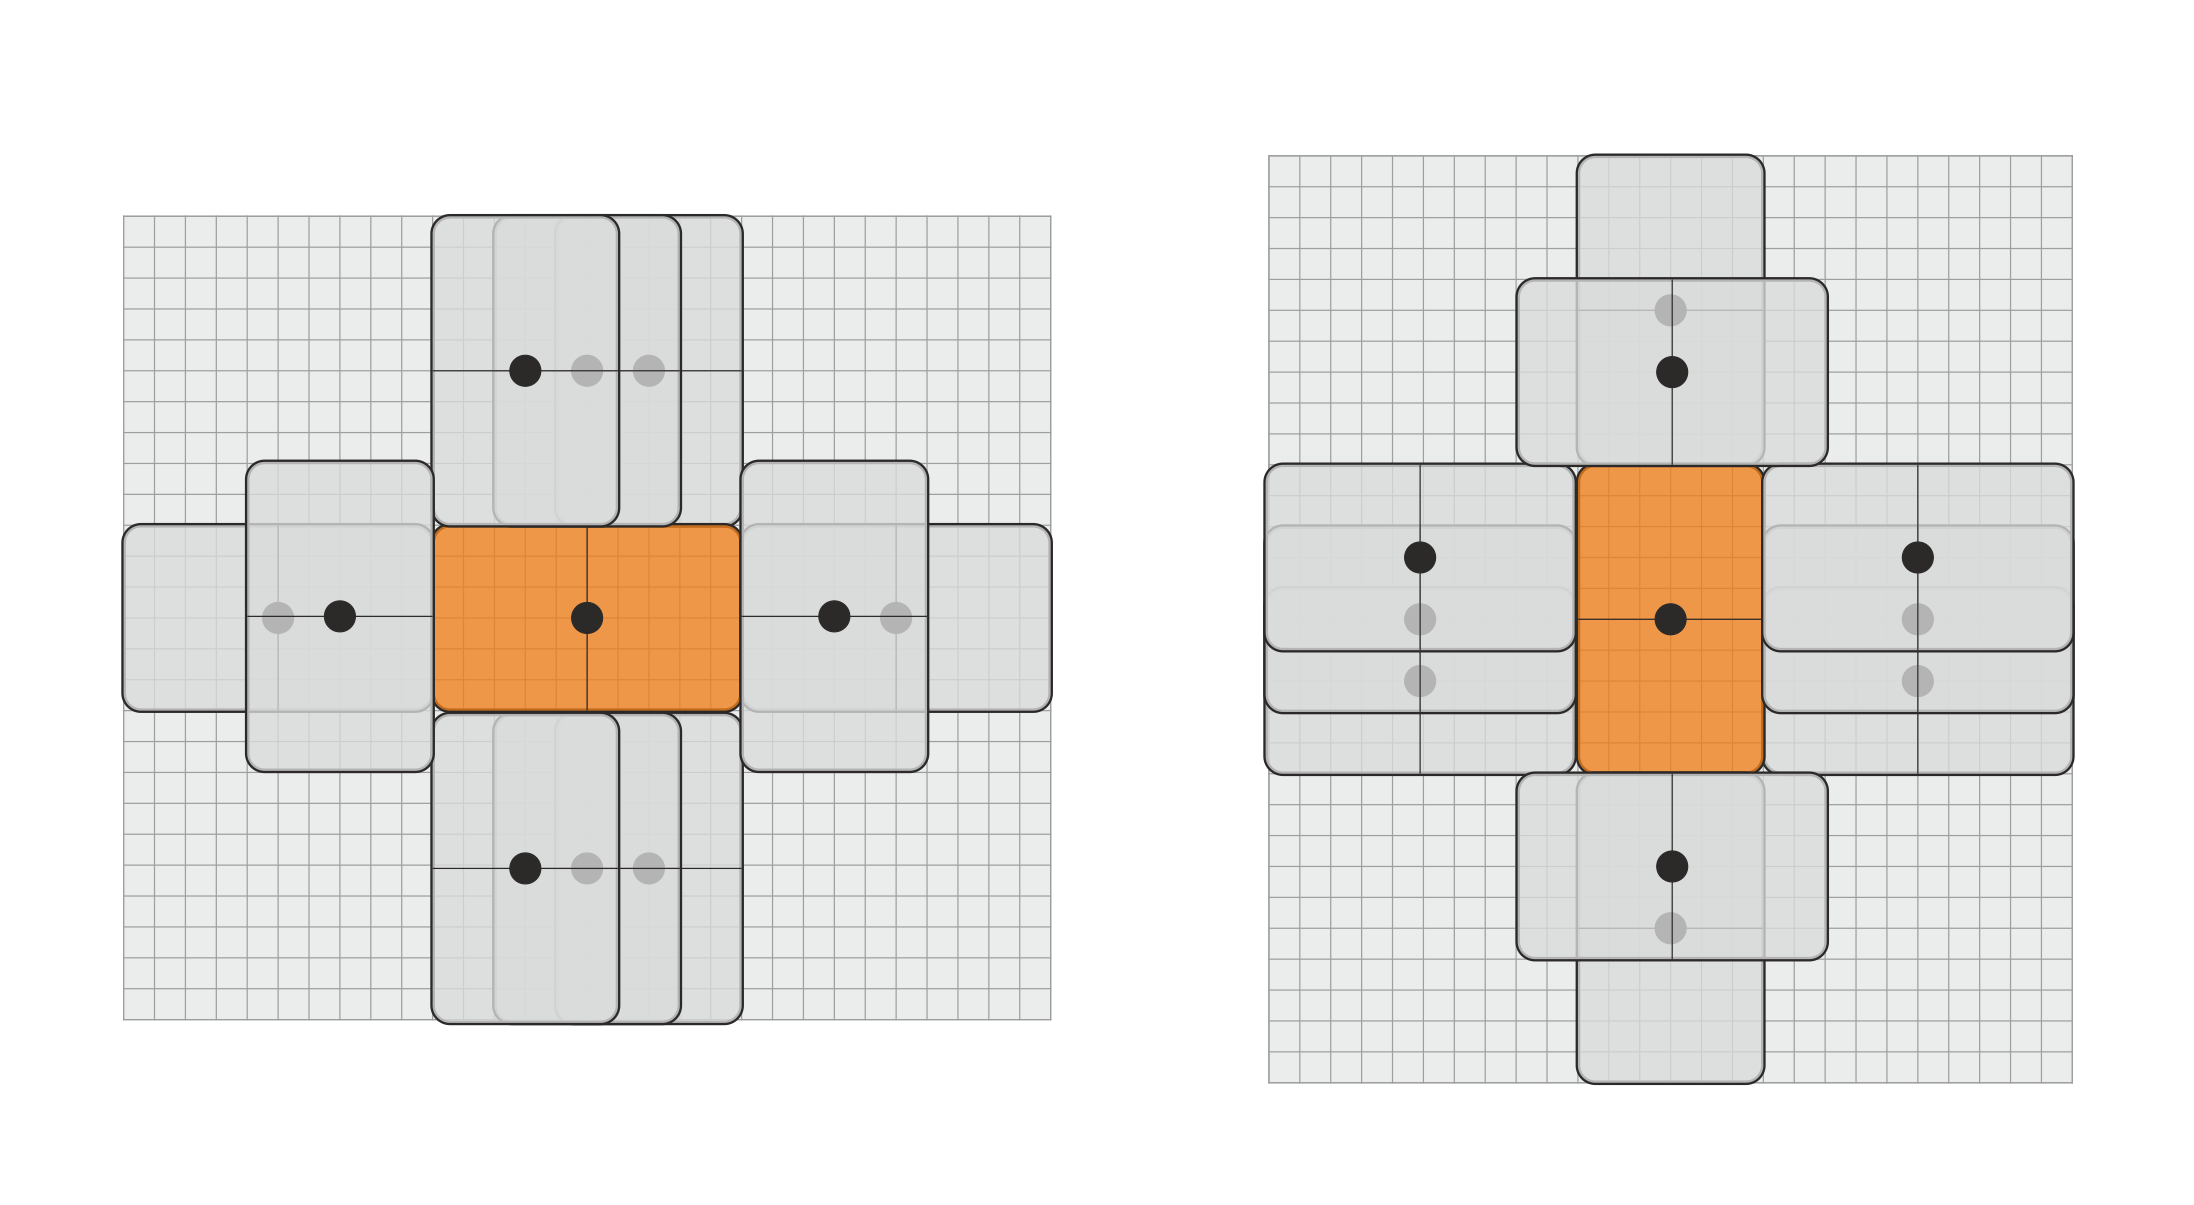
\includegraphics[scale=0.9]{tiles_position.png}
  \end{center}
  \caption{Diferentes posiciones en las que se puede colocar una ficha en el tablero}
  \label{fig:tiles-position}
\end{figure}

Para saber dónde colocar las fichas se necesita información de todas estas variables, y dependiendo del caso, optar por
una posición u otra. Dado que existen multitud de circunstancias y posibles opciones, se decidió encapsular en un método
y realizar todos los cálculos y comprobaciones para luego mover directamente la ficha.

\subsection{Interfaz de sonido}

La interfaz de sonido se ha diseñado de tal forma que se gestione de forma independiente para que su uso sea sencillo,
realizando llamadas al objeto \textbf{sound} con los métodos que estimemos oportunos en cada momento, y el propio
sistema se encarga de realizar diferentes cálculos y comprobaciones:

\begin{itemize} 
    \item Por ejemplo, a la hora de ejecutar un determinado fragmento musical, controla si ya se está escuchando música
        en ese momento; si es ese el caso realiza un pequeño fundido de la pista actual, e inicia la ejecución de la
        nueva, evitando así los desagradables clicks que se podrían escuchar cuando se para y se inicia la canción.
    \item O también, para ejecutar un sonido de ficha de dominó sobre el tablero, el sistema realiza la precarga de todos
        los sonidos --- similares pero no iguales --- y dispara uno aleatoriamente, evitando que cada apartado tenga
        que gestionarlo de forma autónoma
\end{itemize}


\subsection{Configuración de la aplicación}

La configuración de la aplicación (y almacenaje de la misma) se realiza mediante ficheros de tipo \textbf{INI}. Un archivo
INI consiste en un simple archivo de texto ASCII que contiene dos tipos de entradas:

\begin{description}
    \item[Secciones] permiten agrupar parámetros relacionados. Por ejemplo: "Parámetros de red".
    \item[Valores] definen parámetros y su valor. Primero se define el nombre del parámetro y después su valor separado por
            el signo de igualdad (=).
    \item[Comentarios] permiten explicar el propósito de una sección o parámetro. Los comentarios comienzan con el carácter
            punto y coma (;).
\end{description}

El significado de secciones y valores no está bien definido y cada aplicación puede reaccionar de manera diferente ante:

\begin{itemize}
    \item Secciones duplicadas.
    \item Parámetros duplicados.
    \item El carácter de barra invertida (\textbackslash). A veces se usa para romper una línea en dos.
    \item Valores. Los valores pueden consistir en texto, números, listas separadas por comas, etc. Esto depende de la aplicación.
\end{itemize}

Las ventajas de este tipo de ficheros es su estandarización y comodidad a la hora de leer y guardar valores en fichero,
de tal forma que podemos guardar información por defecto sobre el juego de la siguiente forma:

\begin{lstlisting} [caption={Fichero INI de ejemplo}, language=Python, numbers=left]
config.add_section('General')
config.set('General', 'name', 'Dominous')
config.set('General', 'window_caption', 'Dominous')
config.set('General', 'lang', 'en')
config.set('General', 'points_per_game', '200')
config.add_section('Screen')
config.set('Screen', 'window_width', '800')
config.set('Screen', 'window_height', '600')
config.set('Screen', 'full_screen', 'False')
config.set('Screen', 'window_fav', os.path.join('images', 'fav.png'))
config.add_section('Theme')
config.set('Theme', 'theme', 'spanish')
config.add_section('Game')
config.set('Game', 'player2', 'easy')
config.set('Game', 'player3', 'easy')
config.set('Game', 'player4', 'easy')
# write our configuration file to file
with open(file, 'wb') as configfile:
    config.write(configfile)
\end{lstlisting}

Y más tarde leerlo simplemente con:

\begin{lstlisting} [caption={Código Python de lectura de fichero INI},language=Python, numbers=left]
config = ConfigParser.RawConfigParser()
config.read(file)
config_default = {
    'name': config.get('General', 'name'),
    'window_caption': config.get('General', 'window_caption'),
    'window_width': config.getint('Screen', 'window_width'),
    'window_height': config.getint('Screen', 'window_height'),
    'full_screen': config.get('Screen', 'full_screen'),
    'window_favicon': config.get('Screen', 'window_fav'),
    'tile_width': 525,
    'tile_height': 270,
    'scale': 0.2,
    'theme': config.get('Theme', 'theme'),
    'lang': config.get('General', 'lang'),
    'points_per_game': config.get('General', 'points_per_game'),
    'gametype': 'human',
    'gametype_current': 'single',
    'player1': 'easy',
    'player2': 'easy',
    'player3': 'easy',
    'player4': 'easy',
    'speed': '1',
}
\end{lstlisting}

Todo ello encapsulado dentro del módulo \textbf{config.py} de la aplicación.

Con esto conseguimos un sistema para almacenar la configuración del sistema mediante un método portable, cómodo, sencillo y 
editable por el usuario mediante cualquier tipo de editor de texto (en caso de que existiera cualquier tipo de problema).

\subsection{Inteligencia Artificial}

En Dominous, el Sistema Experto de Inteligencia Artificial se reparte entre varios módulos, simplificando la implementación
de las diferentes partes. Según la estructura clásica en las que se divide un Sistema Experto, podemos ver que cada
apartado genera información o conocimiento para la Inteligencia Artificial:

\begin{description}
    \item[Base de conocimientos] Contiene conocimiento modelado extraído del diálogo con un experto --- Esta base de
        conocimiento se almacena, por un lado en la biblioteca de funciones y herramientas para desempeñar una partida,
        y físicamente se almacena en el módulo de IA
    \item[Base de hechos (Memoria de trabajo)] contiene los hechos sobre un problema que se ha descubierto durante el análisis
        --- Los hechos se van creando y almacenando gracias al módulo de \textbf{Gestión de Partida de Dominó}, que
        gobierna la partida y guarda toda la información, movimientos, pasos y tiempos al colocar las fichas.
    \item[Motor de Inferencia] Modela el proceso de razonamiento humano --- gracias a la biblioteca de funciones podemos
        crear un motor de inferencia fácilmente, utilizando pequeñas reglas y dotando de peso o importancia a cada una,
        modelando exactamente el proceso de razonamiento que queramos, e incluso ofertando la posibilidad de crear
        cuantos queramos, de una forma fácil y rápida.
    \item[Módulos de justificación] Explica el razonamiento utilizado por el sistema para llegar a una determinada conclusión
        --- ya que en el dominó no se puede evaluar por sí mismo la efectividad o conveniencia de un movimiento, esta
        justificación llega del conocimiento del experto en valorar con mayor o menor peso una regla.
    \item[Interfaz de usuario] es la interacción entre el Sistema Experto y el usuario, y se realiza mediante el lenguaje
        natural --- y, en el caso de Dominous, la interfaz se comunica con el usuario mediante el módulo del motor
        gráfico del juego, que muestra fichas, movimientos y jugadores.
\end{description}

Pasemos a describir cada apartado para conocer a fondo la implementación del sistema experto.

\subsubsection{Base de conocimientos}

La base de conocimiento se obtiene desde el módulo \textbf{Gestión de Partida de Dominó}, que almacena la información
de forma global, esto es, relativa a toda la partida:

\begin{lstlisting} [caption={Información global de la partida}, language=Python, numbers=left]
self.info = {
    "date" : date,
    "place" : place,
    "max_points" : max_points,
    "player1" : player1,
    "player2" : player2,
    "player3" : player3,
    "player4" : player4,
    "team1" : player1 + " " + player3,
    "team2" : player2 + " " + player4,
    "description" : description,
    "winner_team" : "",
    "team1_points" : 0,
    "team2_points" : 0,
}
\end{lstlisting}

El identificador de cada campo es bastante descriptivo

Y también se almacena información de la mano actual y de cada movimiento de la siguiente forma:

\begin{lstlisting} [caption={Información de la mano actual}, language=Python, numbers=left]
movement = {
    'player' : player,
    'tile' : tile,
    'side' : side,
    'left' : left,
    'right' : right,
    'mtime' : mtime,
}
\end{lstlisting}

Entre los campos almacenados vemos uno que nos resultará de mucho interés en posteriores usos de esta información, y es
el campo \textbf{mtime}. Este campo almacena el tiempo que ha estado el jugador pensando antes de colocar una ficha,
y gracias a que el dominó es un juego de caballeros podemos utilizar esta información para elaborar una estrategia
para conseguir la victoria. \\

Los posibles valores que puede presentar este campo son:

\begin{description}
    \item[0] El usuario no ha requerido tiempo para decidir qué ficha colocaba.
    \item[1] El usuario ha pensado entre diferentes opciones, y ha necesitado de cierto tiempo para decidir la ficha.
    \item[2] El usuario ha utilizado una cantidad de tiempo considerable para decidir la ficha a colocar.
\end{description}

\subsubsection{Base de Hechos}

La Base de Hechos se ha modularizado en pequeñas funciones o reglas, de tal forma que pueden ser fácilmente reutilizadas en
el Sistema Experto de cualquier jugador de Dominous. La estructura básica de una regla es la siguiente:

\begin{lstlisting} [caption={Estructura básica de regla}, language=Python, numbers=left]
class nombre_de_la_regla:
    def __init__(self):
        # inicializamos los atributos que sean necesarios
        pass
    def go(self, left_tile, right_tile, board, tiles, log):
        return ficha, lado, tiempo_pensando
\end{lstlisting}

Como vemos la estructura es sencilla, implementada mediante clases Python, y tiene una inicialización para definir los
atributos que sean necesarios, y por otra parte un método que, para una situación concreta de estado de la partida
(tablero, fichas propias, posición del jugador y toda la información generada por la partida). \\

Veamos un ejemplo práctico. Vamos a definir una regla que intente colocar sobre el tablero una ficha doble, cualquiera
que tengamos. Esta regla se implementaría de la siguiente forma:

\begin{lstlisting} [caption={Regla para colocar ficha doble}, language=Python, numbers=left]
class put_any_double:
    def __init__(self):
        pass
    def go(self, left_tile, right_tile, board, tiles, log):
        for item in tiles:
            if item[0] == item[1]:
                if item[0] == left_tile or item[1] == left_tile:
                    tiles.remove(item)
                    return item, "left", 1
                    break
                elif item[0] == right_tile or \
                    item[1] == right_tile or \
                    left_tile == None:
                    tiles.remove(item)
                    return item, "right", 1
                    break
        return None, "pass", 0
\end{lstlisting}

En la inicialización no requerimos dar de alta ningún atributo, y el método \textbf{go} simplemente comprueba que, para
alguna de nuestras fichas dobles, algún lado de la mesa tenga ese mismo valor. Si lo tiene hemos conseguido realizar
esta regla, devolvemos el valor y listo. Y si no, devolvemos una señal de que no hemos tenido éxito y salimos. \\

Gracias a este sistema, simplificamos mucho el desarrollo de nuevos Sistemas Expertos, ya que:
\begin{itemize}
    \item Es muy sencillo crear nuevas reglas. Como ya vimos en El Libro del dominó de Benito Ruipérez \cite{mora90},
        muchas reglas, funciones o herramientas se basan en frases o hechos que, si se cumplen, \emph{interesa}
        \footnote{Como vemos, debemos ser cuidadosos al emplear verbos como \emph{interesa} o \emph{debemos} al hablar
        de colocar fichas. El juego del Dominó es lo suficientemente complejo y goza de muchas estrategias como para poder
        simplificarlo o decir objetivamente que debemos realizar una acción.} cumplirlos.
        Por poner un caso simple, al comenzar la partida \emph{interesa} comenzar con un doble --- o, mejor dicho, hay
        estrategias interesadas en comenzar con un doble. Para emplear este razonamiento en estas estrategias simplemente
        tenemos que añadir esta regla con el peso suficiente, y ya lo tendremos implementado.
    \item Es fácil crear nuevos sistemas, creando pilas de reglas con pesos que se van disparando si pueden cumplirse.
        Así se van creando diferentes jugadores y dotamos al juego de más variedad y diversión.
\end{itemize}

Los jugadores poseen una lista de elementos, utilizando normalmente la nomenclatura \textbf{self.knowledge}, y van
añadiendo las reglas que estimen oportunas como si fuera una lista clásica de Python, utilizando el método \textbf{append}. \\

Si estamos desarrollando un jugador simple, podemos definir su base de conocimiento de la siguiente forma:

\begin{lstlisting} [caption={Base de conocimiento simple}, language=Python, numbers=left]
self.knowledge = []
self.knowledge.append([put_any_double()])
self.knowledge.append([put_anyone()])
\end{lstlisting}

Como vemos, estamos definiendo que el jugador intente, inicialmente, colocar una ficha doble. Si esto no es posible,
intentará colocar una ficha cualquiera. \\

Así, con solamente tres líneas podemos comenzar a desarrollar una inteligencia artificial a nuestro gusto, que juegue
y valore cada regla con la importancia que estimemos oportuna. \\

Por otro lado, también podemos utilizar reglas con el mismo peso, dotando de aleatoriedad al jugador y permitiendo
que se comporte de diferente modo en situaciones similares. De este modo, si queremos definir a un jugador un poco
más complejo, su base de conocimiento podría escribirse así:

\begin{lstlisting} [caption={Base de conocimiento compleja}, language=Python, numbers=left]
self.knowledge = []
self.knowledge.append([
    put_any_double(),
    weight_matrix()
])
self.knowledge.append([put_anyone()])
\end{lstlisting}

En un primer momento se ejecutará, aleatoriamente, una regla entre \textbf{put\_any\_double()} y \textbf{weight\_matrix()}.
Si no hay suerte con la primera, se intentará con la segunda, y si no hay éxito con ninguna se ejecutará el siguiente
conjunto de reglas --- en este caso, \textbf{put\_anyone()}, es decir, intentar colocar una ficha cualquiera.

El Motor de Inferencia se desarrolla de forma muy sencilla, ya que se utilizan estructuras muy simples proporcionadas
por el mismo lenguaje Python. \\

\subsubsection{Motor de Inferencia}

El Motor de Inferencia es el encargado de elegir una regla de entre todas las reglas definidas en la Base de Conocimiento
del jugador concreto. Este motor, antes de evaluar cualquier regla, realiza diferentes comprobaciones para acelerar
los tiempos de cálculo en ciertos casos especiales. Así, las reglas no se evaluarán bajo las siguientes circunstancias:
\begin{itemize}
    \item El jugador no puede colocar ninguna ficha --- si ninguna de las fichas que posee el jugador son candidatas
        a utilizarse en el tablero, el Motor de Inferencia pasará automáticamente el turno al siguiente jugador.
    \item El jugador solo puede colocar una ficha ---  en el caso de que solamente una ficha sea candidata a colocarse
        en juego, el sistema la colocará automáticamente, dando la información de que el jugador ha estado poco tiempo
        pensando qué ficha colocar, y pasará el turno al siguiente jugador.
\end{itemize}

Solamente en el caso de que más de una ficha sea candidata a colocarse, el Motor de Inferencia hará uso de la Base
de Conocimiento y aplicará las reglas del sistema experto.

\subsection{Música y efectos}

La música también juega un papel importante en un videojuego, y no debe ser elegida a la ligera, sino
        debe buscarse una razón y un estilo que encaje con los objetivos definidos. Esta aplicación está orientada a un
        público muy general, y el ritmo del juego es tranquilo y pausado, así que se eligió el jazz como estilo base
        para acompañar al juego.

\begin{figure}[h]
  \label{jamendo}
  \begin{center}
    
\includegraphics[scale=0.8]{jamendo.jpg}
  \end{center}
  \caption{La música se obtuvo de Jamendo, un servicio de música libre}
\end{figure}

        Gracias a la enorme comunidad de músicos que publican sus obras con \emph{licencias libres}
        --- permitiendo que sus obras se utilicen y se adapten a otros entornos --- no fue nada complicado buscar
        un conjunto de canciones que se adaptaran al ritmo y velocidad que se disfruta en Dominous. \\

        En cuanto a los efectos de sonido la cosa estuvo un poco más complicada. Al inicio se buscaron sonidos que
        pudieran encajar con las acciones de colocar la ficha, y se probó con efectos de sonido clásicos de click --- sonidos
        cortos que informan de una acción --- pero se descubrió que, aunque dotaban de la suficiente información
        al usuario, no quedaban bien con la estructura y estilo de Dominous. \\

        La solución que se tomó fue grabar sonidos reales de fichas de dominó golpeando una mesa. Una vez se contó con
        un buen grupo de sonidos, se eligió uno como candidato un golpe seco, limpio y con sonoridad. Pero descubrimos
        que escuchar siempre el mismo sonido era molesto para el usuario (y muy poco realista), así que se optó por mejorar
        la solución final: elegir un gran conjunto de sonidos diferentes de fichas de dominó y ejecutar aleatoriamente
        uno de ellos cada vez que la ficha golpeaba la mesa. \\
        
        Así conseguimos una sonoridad y aleatoriedad agradable para el usuario.


\chapter{Pruebas}
% -*-cap2.tex-*-
% Este fichero es parte de la plantilla LaTeX para
% la realización de Proyectos Final de Carrera, protegido
% bajo los términos de la licencia GFDL.
% Para más información, la licencia completa viene incluida en el
% fichero fdl-1.3.tex

% Copyright (C) 2009 Pablo Recio Quijano 

\section{Pruebas}

La fase de prueba es de las más importantes de un proyecto software~\cite{art}. El objetivo de este paso es, como razón
última, la verificación de que el proyecto cumple con todos los requisitos iniciales que se plantearon al comienzo 
del desarrollo. Según la metodología clásica de desarrollo de pruebas existen diferentes enfoques a la hora de realizar
este tipo de pruebas de software, siendo todos complementarios~\cite{beizer_software_1990}, pero para el caso
concreto que tenemos entre manos debemos tener en cuenta la naturaleza del proyecto. \\

Los videojuegos presentan dos facetas distintas que deben ser abordadas de diferentes maneras cuando se realiza la fase
de pruebas:
\begin{itemize}
    \item Por un lado tenemos las pruebas clásicas que se realizan a cualquier desarrollo de software, como pueden
            ser las pruebas unitarias o de integración, destinadas a verificar el correcto funcionamiento del
            código.
    \item Y por otro lado, al requerir de una interacción directa con el usuario (y estar destinado a divertir,
            entretener y proporcionar un rato ameno al mismo) se deben realizar varios tipos de pruebas orientadas
            a comprobar que se cumplen requisitos más abstractos como puede ser el testeo o análisis de la jugabilidad
            o usabilidad de la aplicación, interfaces, medir el entretenimiento que proporciona la aplicación (relacionado
            directamente con el desarrollo de la inteligencia artificial de los contrincantes, entre otros)
\end{itemize}

El primer conjunto de pruebas se pueden realizar con comprobaciones de código, compilación (o en este caso concreto,
interpretación) del mismo y diferentes métodos, pero el segundo conjunto de pruebas es necesario que se desarrollen
con diferentes tipos de usuarios reales manejando la aplicación y realizando cuestionarios que nos ayuden a valorar
el éxito o fracaso de estos apartados. \\

Para los apartados de pruebas unitarias y de integración se va a trabajar principalmente con los tres módulos que
forman el núcleo fuerte de la aplicación (y sobre las que cae el peso de la misma):

\begin{itemize}
    \item Sistema de gestión de partida de dominó
    \item Sistema de inteligencia artificial
    \item Motor gráfico de la aplicación
\end{itemize}

\subsection{Pruebas unitarias}

Durante la fase de implementación se fueron realizando pruebas unitarias no automatizadas de cada conjunto o subconjunto
de módulos que se iban desarrollando, evitando así encontrar errores en las pruebas de integración que no sean propiamente
de integración sino de errores en la codificación de los diferentes módulos. \\

Una herramienta cuyo uso ha resultado muy interesante y útil ha sido \textbf{PyFlakes}. Esta herramienta es un programa que
analiza otros programas escritos en Python y detecta un gran conjunto de errores analizando el código fuente. Existen otras
herramientas de análisis automático de código Python, como PyChecker o PyLint, pero se decidió utilizar PyFlakes
principalmente por la rapidez de análisis y seguridad ante caídas, ya que no requiere ejecutar el código, sino que realiza
un análisis mediante \emph{parseo} del código. \\

En cuanto a los diferentes módulos que conforman Dominous, existen varios casos inherentes a cada módulo que deben
tratarse de forma individual (ya que dependen de la naturaleza del módulo) y de forma manual (ya que no se puede abordar su
solución de forma automática).

\subsubsection{Sistema de gestión de partida de dominó}

En este módulo las pruebas unitarias están claras: el módulo debe velar por el correcto cumplimiento de todas y cada
una de las reglas del dominó internacional. Para ello debe vigilarse cada movimiento de los jugadores, repasando
el estado del juego y las diferentes posibilidades que tiene el jugador, entrándose en modo error cuando se realiza
una acción ilegal. \\

En este momento del desarrollo se tuvo que tomar una decisión respecto a cómo contemplar los errores o incumplimiento de
normas que puedan producirse (de forma intencionada o no) por parte de los jugadores:

\begin{itemize}
    \item Una opción era permitir que los jugadores incumplan las normas y actuar en consecuencia contra el jugador.
            En ningún momento se puede permitir que los jugadores coloquen fichas en lugares donde está prohibido
            ese movimiento, por lo que, de todas las normas que posee el dominó las únicas candidatas a entrar en este
            grupo son las que hacen del dominó un \textbf{juego de señores}, es decir, todas aquellas que están destinadas
            a dotar de información a los demás jugadores de forma obligatoria (como puede ser la falta de un palo mediante
            acortar el tiempo que transcurre en su turno).

            Para esta opción teníamos nuevamente otras dos opciones:
            \begin{itemize}
                \item Podemos permitir y \emph{mirar hacia otro lado}, permitiendo que los jugadores engañen de forma
                        clara a los demás jugadores, incluyendo compañeros, o
                \item Podemos actuar como jueces y penalizar a los jugadores que cometan este tipo de faltas.
            \end{itemize}
    \item La otra opción es no permitir este tipo de acciones, volviendo hacia atrás en la acción del jugador y
            pidiendo de nuevo que actúe, hasta que la acción satisfaga las reglas del juego del dominó.
\end{itemize}

Finalmente se decidió que, dado que esta aplicación tiene como requisito el favorecer el aprendizaje del juego del dominó,
no existe cabida alguna a jugadas deshonrosas o que puedan llevar a equivocación al usuario que desea aprender a jugar. \\

Por lo tanto, cuando un jugador intenta realizar una acción equivocada, se deshace esa acción y se le pide de nuevo que
mueva ficha hasta que ese movimiento sea correcto, momento en el cual se continúa con naturalidad la partida.


\subsubsection{Sistema de Inteligencia Artificial}

El juego del dominó es un juego con un amplio universo de acciones y con conocimiento limitado de la situación de la partida,
por lo que no se puede estimar que una acción sea óptima (puede haber varias opciones válidas). Pero a pesar de esto sí existe
un requisito que debe cumplirse (y se exige el cumplimiento) a la hora de realizar un movimiento, y es o pasar o colocar una
ficha cualquiera que pueda colocarse. \\

Esta acción se definió y se tomó como opción por defecto (también llamado fallback) en caso de que todas las demás reglas
de Inetligencia Artificial no se cumplan, y antes de que el sistema quede colgado o no se pueda continuar, se toma esta acción y se continúa
con la partida.


\subsection{Pruebas de integración}

Según se iban desarrollando módulos y éstos cumplían las pruebas unitarias desarrolladas para estos apartados, era necesario
integrar los diferentes módulos para corroborar y contrastar el correcto funcionamiento de la conjunción de ambos módulos.

\begin{figure}[h]
  \begin{center}
    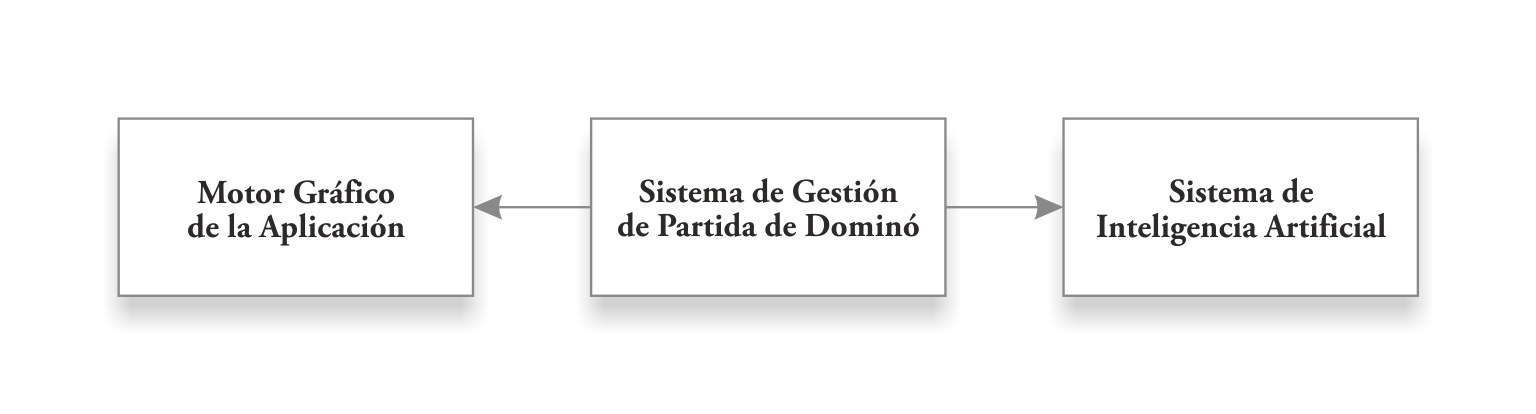
\includegraphics[scale=1.3]{pruebas_integracion.png}
  \end{center}
  \caption{Esquema de relaciones entre módulos para las pruebas de integración}
  \label{pruebas_integracion}
\end{figure}

\subsubsection{Sistema de Gestión de Partida de Dominó y Sistema de Inteligencia Artificial}

Una vez definida la interfaz de comunicación entre el Sistema de Gestión de Partida de Dominó y Sistema de Inteligencia
Artificial, para comprobar la consistencia de esta integración se desarrolló un jugador de dominó muy simple que debía
cumplir con dos premisas:

\begin{enumerate}
    \item El jugador debe cumplir con éxito las especificaciones de la interfaz.
    \item El jugador debe poner una ficha cualquiera (si puede colocar una ficha) o debe pasar (si no existe la posibilidad
            de mover).
\end{enumerate}

Durante el desarrollo del Sistema de Gestión de Partida de Dominó se fue comprobando el éxito de la comunicación entre ambos
módulos, de tal modo que cuando se realizó la integración con los dos sistemas totalmente finalizados no se encontraron
problemas graves, obteniéndose una integración suave y sin errores costosos de solventar.

\subsubsection{Sistema de Gestión de Partida de Dominó y Motor gráfico de la aplicación}

La integración fue más costosa que la comentada anteriormente, ya que no se pudo realizar un sistema de pruebas que
cumpliera las especificaciones de integración, pero gracias a que el Sistema de Gestión de Partida de Dominó contaba
con un gran número de métodos de todo tipo para obtener información del estado del tablero, jugadores y otros,
se pudo realizar la integración de forma sencilla y sin retrasarnos en demasía en la estimación de tiempos.


\subsection{Pruebas de Jugabilidad, usabilidad y experiencia de usuario}

La jugabilidad en Dominous abarca dos ámbitos diferenciados: por un lado se desea que el juego transcurra fluido, sin
parones bruscos o bajadas en la velocidad de cálculo y dibujado de la pantalla, y por otro lado que el jugador, al mover
fichas y desenvolverse por el juego y los menús. \\

El desempeño o velocidad de la aplicación está asegurado por varios factores:

\begin{itemize}
    \item Utilización de una librería de bajo nivel como es PyGame, cuya velocidad está garantizada y testeada en profundidad.
    \item La naturaleza propia de la aplicación, que se desarrolla a un ritmo bajo, no necesita de grandes cálculos ni
            uso avanzado de la CPU.
    \item El motor de inteligencia artificial es rápido, y en casos en los que las posibilidades del usuario se limiten
            a pasar o colocar una única ficha, el motor salta todas las comprobaciones de reglas que sabe que van a
            fallar --- redundando así en una mayor velocidad y rendimiento.
\end{itemize}

\begin{figure}[h]
  \begin{center}
    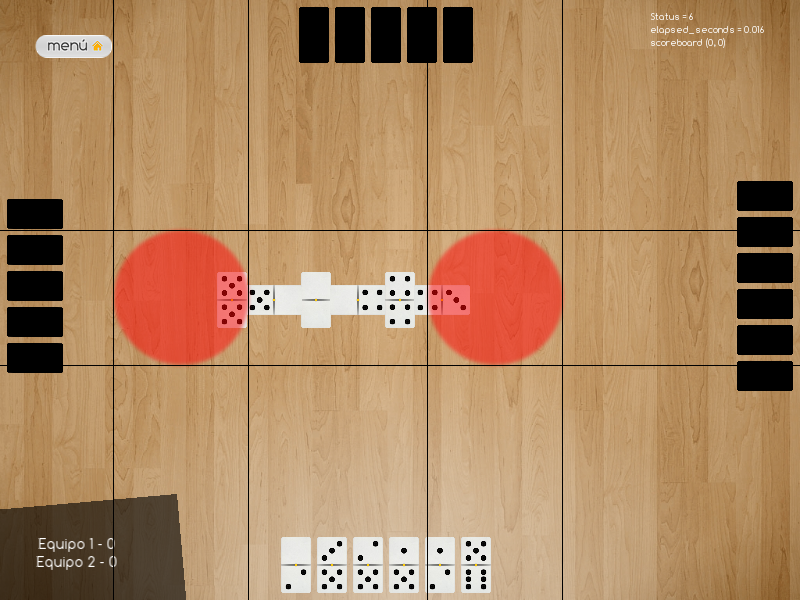
\includegraphics[scale=0.8]{superficie_drop.png}
  \end{center}
  \caption{Superficie sobre la cual el usuario puede dejar la ficha satisfactoriamente}
  \label{superficie_drop}
\end{figure}


La jugabilidad de la aplicación, dado que la acción más común que realizará el usuario será mover las fichas,
se trabajó haciendo que el movimiento de arrastrar y soltar la ficha sea satisfactorio, cuidando que la ficha siga
al cursor de forma fiel, el error de soltar una ficha en un lugar equivocado no sea frustrante --- sino que se convierta
en un hecho más de la partida ---, que la zona donde el usuario suelta la ficha sea grande y no se produzcan errores
no deseados y funcionalidades y pequeñas mejoras que buscan que el jugador se divierta con la aplicación. \\

\begin{figure}[h]
  \begin{center}
    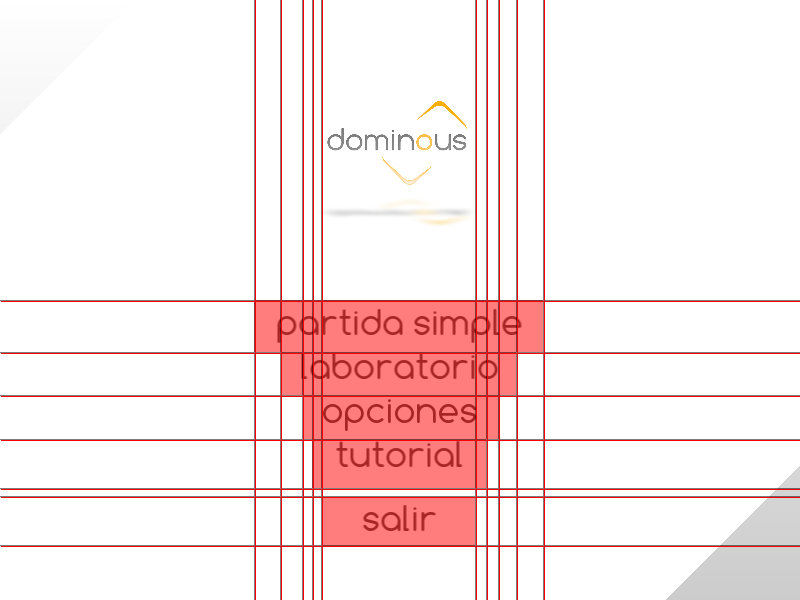
\includegraphics[scale=0.8]{superficie_click.png}
  \end{center}
  \caption{Como vemos, la superficie en la cual el usuario puede realizar click de forma satisfactoria es más amplia que el simple texto que incluye}
  \label{superficie_click}
\end{figure}

Dado que la aplicación está orientado a un público adulto --- que, probablemente, no goce de una habilidad muy desarrollada
con los dispositivos de entrada --- la zona de click sobre menús y demás elementos de la interfaz se ha agrandado, con lo
cual las posibilidades de éxito del click aumentan, así como la satisfacción del usuario con la herramienta. \\

Por último, se han realizado numerosas pruebas con usuarios reales durante el desarrollo del proyecto, recibiendo
feedback real y realizando y estudiando pequeñas modificaciones que hagan que el mismo disfrute de la experiencia de
jugar a este producto. \\

Los usuarios sobre los que se han realizado las diferentes pruebas son los siguientes:

\begin{description}
    \item[Sujeto 1] Mujer, 28 años, estudios universitarios de la rama de letras, nivel de informática usuario alto, con conocimientos
        de ofimática, poca experiencia en videojuegos, bajo nivel de las reglas y normas del dominó internacional.
    \item[Sujeto 2] Hombre, 63 años, estudios universitarios de economía, nivel de informática usuario medio, nula experiencia en
        videojuegos, jugador experimentado de dominó.
    \item[Sujeto 3] Hombre, 30 años, estudios universitarios de Informática, alto nivel de informática usuario, amplia experiencia
        en videojuegos, nivel medio de conocimiento del juego de dominó.
    \item[Sujeto 4] Hombre, 31 años, estudios universitarios de Informática, alto nivel de informática usuario, amplia experiencia
        en videojuegos, nivel bajo de conocimiento del juego de dominó.

\end{description}

Se analizó el uso de la aplicación por parte de los sujetos con las siguientes circunstancias:

\begin{itemize}
    \item Todas las pruebas se realizaron en un ordenador portátil con ratón, ejecutándose la aplicación en un entorno Windows 7.
    \item Se les proporcionó la aplicación ya en ejecución, mostrándoles la pantalla de inicio.
    \item No se les facilitó ningún tipo de información adicional sobre cómo funciona la aplicación.
\end{itemize}

Por otra parte, los objetivos a cumplir eran los siguientes:

\begin{description}
    \item[Objetivo 1] Comenzar una partida simple, jugar una mano, salir al menú principal y cerrar la aplicación.
    \item[Objetivo 2] Cambiar el tema gráfico, seleccionando el tema \textbf{fruits} comenzar una partida simple,
            jugar una mano, salir al menú principal y cerrar la aplicación.
    \item[Objetivo 3] Seleccionar el modo \textbf{solo computadora} en velocidad rápida, visualizar una mano, salir
            al menú principal y cerrar la aplicación.
    \item[Objetivo 4] Entrar en \textbf{laboratorio}, hacer que compitan dos equipos diferentes y comentar con el
            entrevistador cuál de los dos equipos ha conseguido más victorias.
\end{description}

Y los éxitos de objetivos y resultados obtenidos se detallan a continuación:

\begin{description}
    \item[Objetivo 1] Todos los sujetos fueron capaces de completar con éxito el objetivo 1. Cabe destacar que los sujetos
            tres y cuatro salieron al menú principal activando el menú de juego con la tecla \textbf{escape}, y el
            sujeto cuatro salió de la aplicación cerrando directamente la ventana de la misma, sin hacer uso del
            botón salir que se encuentra en el menú principal de Dominous.
    \item[Objetivo 2] Todos los sujetos fueron capaces de completar con éxito el objetivo 2, aunque el usuario dos
            necesitó de información acerca de qué es un tema gráfico --- la información se le proporcionó debido a que el
            bajo nivel de conocimiento informático no permitía el éxito de este objetivo.
    \item[Objetivo 3] Todos los sujetos fueron capaces de completar con éxito este objetivo, pero se produjeron los
            siguientes hechos meritorios de ser comentados:
            \begin{itemize}
                \item El usuario dos se sintió desconcertado cuando se iban produciendo los movimientos automáticos
                    de los jugadores, y preguntó que qué utilidad podía tener ver una partida a esta velocidad y sin
                    participar.
                \item El usuario uno de frustró y preguntó cómo podía salir de la aplicación, a pesar de que la interfaz
                    para volver al menú principal era la misma que en el modo de juego simple.
            \end{itemize}
    \item[Objetivo 4] Los usuarios uno, tres y cuatro completaron con éxito este objetivo. El usuario dos no fue
            capaz de comprender el significado de la gráfica o de las barras, y no entendió el uso que podía tener el
            enfrentar a dos equipos si no puedes ver el transcurso de las partidas.
\end{description}


\chapter{Conclusiones}
% -*-cap2.tex-*-
% Este fichero es parte de la plantilla LaTeX para
% la realización de Proyectos Final de Carrera, protegido
% bajo los términos de la licencia GFDL.
% Para más información, la licencia completa viene incluida en el
% fichero fdl-1.3.tex

% Copyright (C) 2009 Pablo Recio Quijano 

\section{Resultados obtenidos}

Primer simulador de dominó libre.

Aplicación de lo aprendido en la carrera. En especial, ampliación de los conceptos de IA estudiados ¿Llegaste a hacer la asignatura?.

Aprendizaje del juego de dominó.

Primer proyecto que realizo de manera íntegra.

\section{Trabajos futuros}

Juego en red.

Servidor web para compartir sistemas expertos.

Analizador de partidas con aprendizaje automático.



%\backmatter % Apéndices, bibliografia ...

\appendix

\chapter{Manual de instalación}
% -*-cap2.tex-*-
% Este fichero es parte de la plantilla LaTeX para
% la realización de Proyectos Final de Carrera, protejido
% bajo los términos de la licencia GFDL.
% Para más información, la licencia completa viene incluida en el
% fichero fdl-1.3.tex

% Copyright (C) 2009 Pablo Recio Quijano 

\section{Apéndices}


\chapter{Manual de usuario}
% -*-cap2.tex-*-
% Este fichero es parte de la plantilla LaTeX para
% la realización de Proyectos Final de Carrera, protegido
% bajo los términos de la licencia GFDL.
% Para más información, la licencia completa viene incluida en el
% fichero fdl-1.3.tex

% Copyright (C) 2009 Pablo Recio Quijano 

% MANUAL DE USUARIO

% FIXME
% subir al apartado de ficheros de RedIRIS los manuales

\section{Ejecución}

En este capítulo veremos el funcionamiento de la aplicación desde el punto de vista de un usuario final que ejecutará el
videojuego con la intención de disfrutar de las opciones que ofrece. \\

Si el programa está instalado, se ejecuta con:

\begin{lstlisting} [language=Bash, numbers=left]
user@machine:~$ python dominous.py
\end{lstlisting}

o con un simple doble click si nos encontramos en un entorno windows. \\

\section{Menú principal}

El menú principal ofrece las siguientes opciones:

\begin{figure}[h]
  \label{screenshots_menu}
  \begin{center}
    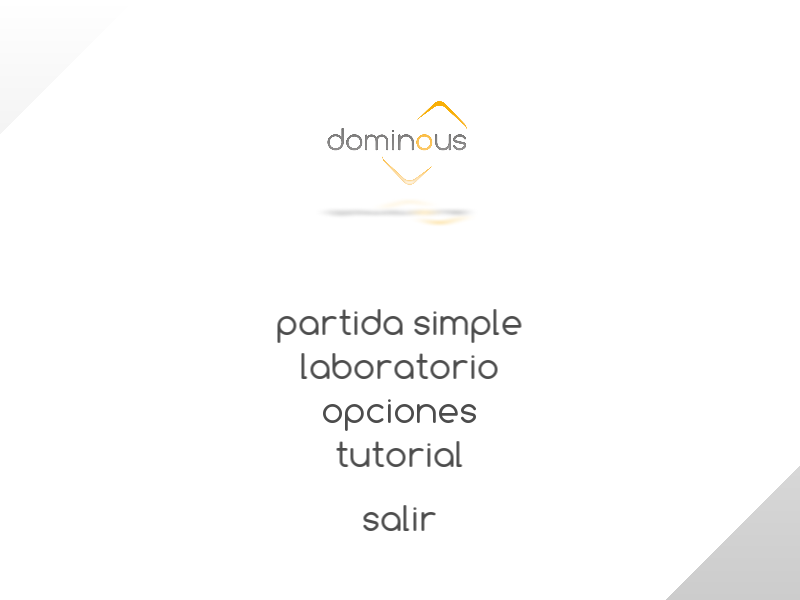
\includegraphics[scale=0.8]{screenshots_menu.png}
  \end{center}
  \caption{Menú principal de Dominous}
\end{figure}

\begin{description}
    \item[Partida simple] Será la poción más utilizada, ya que permite al usuario disfrutar de una partida de dominó.
    \item[Laboratorio] El modo laboratorio enfrenta a dos equipos controlados por el ordenador a cien partidas, para
            intentar dilucidar qué equipo es mejor.
    \item[Opciones] Las opciones del juego nos permite configurar la partida a nuestras necesidades, como veremos en el
            siguiente apartado.
    \item[Tutorial] Nos muestra un conjunto de diapositivas o transparencias con información rápida sobre cómo jugar,
            qué nos ofrece Dominous y unas breves nociones de juego del dominó.
    \item[Salir] Cierra y sale del juego.
\end{description}

Para movernos entre las distintas opciones simplemente debemos utilizar el ratón e ir clicando en las diferentes secciones,
pulsando el botón volver para retornar al menú principal en cualquier momento. Continuemos el manual mostrando la sección
tutorial y viendo las opciones que nos ofrece.

\section{Opciones}

Las opciones de juego, tal y como hemos comentado previamente, nos permite adaptar diferentes opciones de Dominous según
nuestras necesidades. Las opciones que se muestran son las siguientes:

\begin{figure}[h]
  \label{screenshots_options}
  \begin{center}
    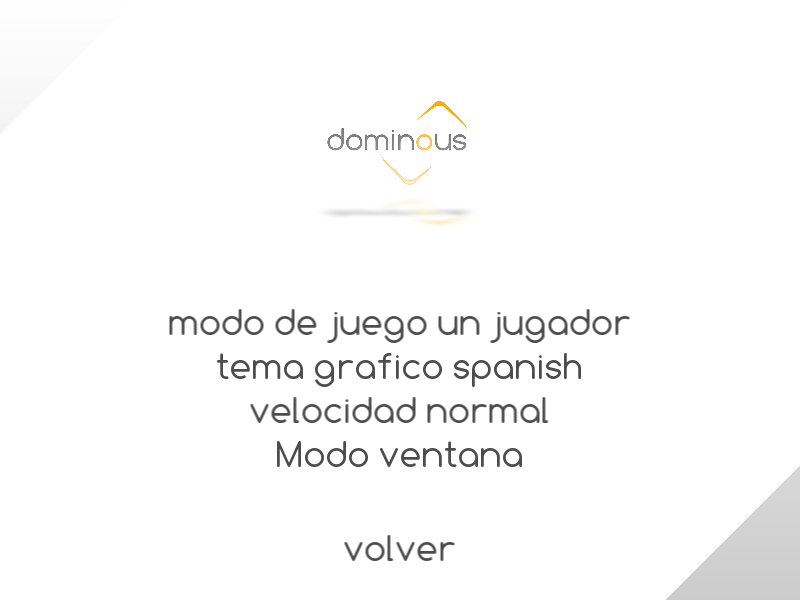
\includegraphics[scale=0.8]{screenshots_options.png}
  \end{center}
  \caption{Pantalla de opciones de juego}
\end{figure}

\begin{description}
    \item[Modo de juego] Podemos seleccionar si, en el modo de juego \textbf{partida simple}, queremos participar nosotros
        como jugador activo o simplemente queremos observar cómo el ordenador desarrolla la partida completa, controlando
        él mismo a todos los jugadores. 
    \item[Tema gráfico] Esta opción nos permite seleccionar el aspecto gráfico de la partida. El aspecto gráfico permite
        cambiar la visualización de fichas, mesa de juego y otros elementos, al estilo de los temas gráficos que poseen
        los sistemas operativos.
    \item[Velocidad de juego] Dominous posee tres tipos de velocidades de juego:
        \begin{itemize}
            \item Velocidad normal --- el juego se desarrolla a una velocidad pausada, con movimientos de fichas que permiten
                seguir el transcurso de la partida con comodidad, y se muestra información sobre el tiempo que emplea cada
                jugador mientras piensa la jugada a ejecutar.
            \item Velocidad rápida --- las fichas se mueven a la misma velocidad que en el modo normal, pero los jugadores
                colocan la ficha inmediatamente en cuanto les toca su turno.
            \item Velocidad extra rápida --- el movimiento de las fichas es acelerado y los jugadores no emplean tiempo
                pensando la jugada
        \end{itemize}
    \item[Modo ventana] Lorem ipsum dolor
\end{description}

\begin{figure}[h]
  \label{screenshots_themes}
  \begin{center}
    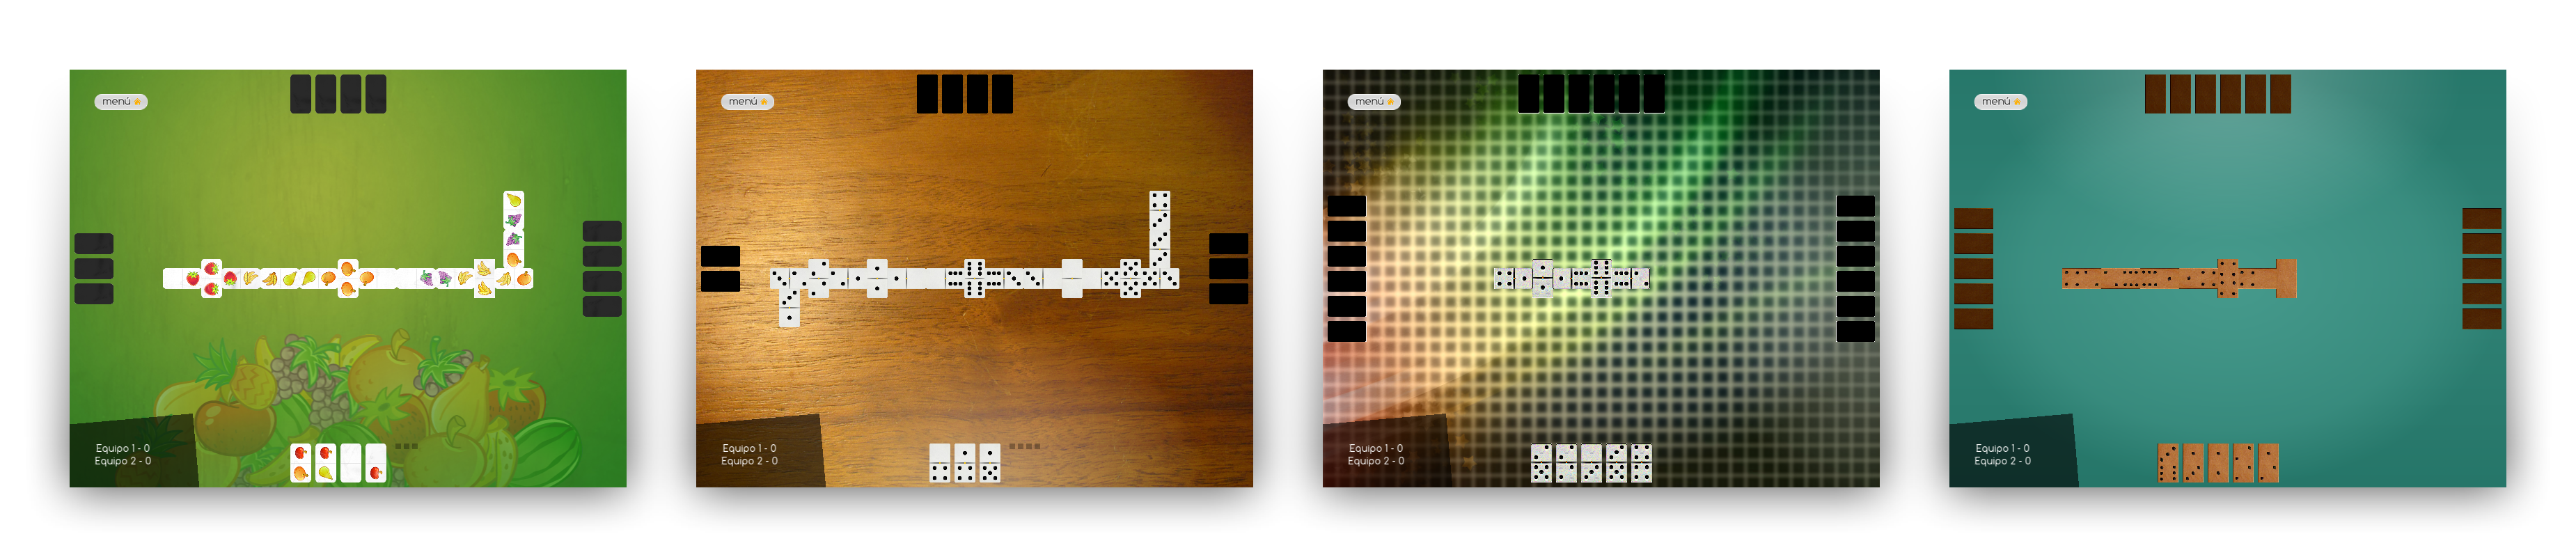
\includegraphics[scale=0.15]{screenshots_themes.png}
  \end{center}
  \caption{Diferentes temas gráficos que vienen de serie con Dominous}
\end{figure}

\section{Tutorial}

El tutorial de juego sirve de ayuda a los nuevos jugadores de Dominous, presentando de forma resumida todas las opciones
que posee Dominous y evitando que, en un primer uso, sea necesario leer todo el manual de usuario.

\begin{figure}[h]
  \label{screenshots_tutorial}
  \begin{center}
    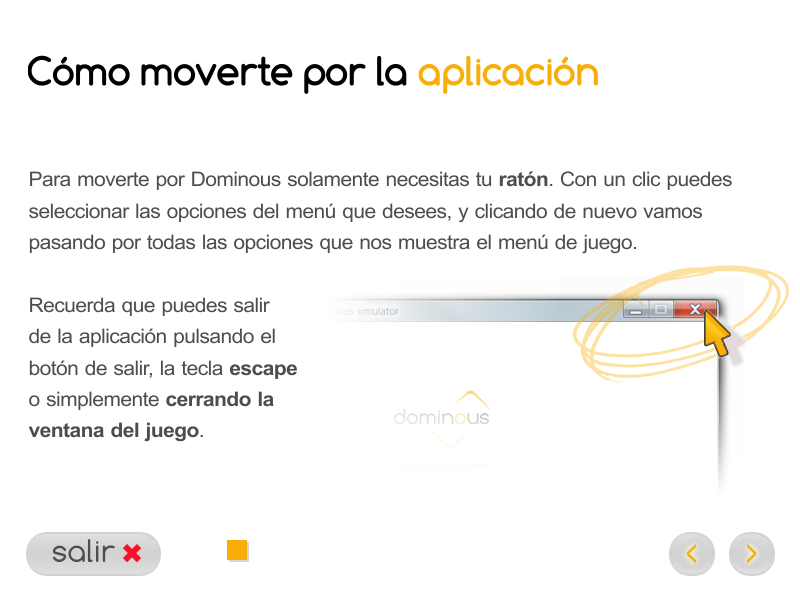
\includegraphics[scale=0.8]{screenshots_tutorial.png}
  \end{center}
  \caption{Modo tutorial, con instrucciones básicas de juego}
\end{figure}

\begin{itemize}
    \item Las primeras capturas informan sobre la interfaz de Dominous: cómo moverte por las opciones, salir del juego, jugar
        una partida, colocar fichas, entrar y salir de una partida de dominó, y diferentes elementos que se muestran a la
        hora de disfrutar de una partida.
    \item Luego se nos informa del modo Laboratorio, describiendo cada uno de los elementos que aparecen en pantalla como
        son las barras de información o la gráfica de partidas ganadas.
    \item Por último se pretende dar al usuario novel de unas nociones básicas de dominó: cómo jugar, cuántas fichas existen,
        breve explicación sobre el modo de juego por parejas y cierres.
\end{itemize}




%\addcontentsline{toc}{chapter}{Software usado}
%\chapter*{Software utilizado}
%% -*-programas.tex-*-
% Este fichero es parte de la plantilla LaTeX para
% la realización de Proyectos Final de Carrera, protegido
% bajo los términos de la licencia GFDL.
% Para más información, la licencia completa viene incluida en el
% fichero fdl-1.3.tex

% Copyright (C) 2009 Pablo Recio Quijano 
Es usual en un PFC referenciar que software has usado para la
realización del mismo. Aprovecharé este apartado para que conozcas
alguna herramienta que puede serte de ayuda para realizar tus
documentos en \LaTeX{}

\section*{Emacs + Auc\TeX}

Emacs es uno de los programas de edición más usados por
desarrolladores de software, ya que es bastante versatil admitiendo
gran cantidad de ``plugins'' o extensiones que permiten ampliar aun
más sus funcionalidades.\\

Uno de estos plugins es Auc\TeX \cite{pdf:auctex}, el cual incluye
rutas para ciertos comandos, resaltado de sintaxis, previsualización
del documento, menú matemático en el cual podemos acceder e insertar
la gran mayoria de los símbolos matemáticos, para no tener que
memorizarlos. Podemos ver un ejemplo de Emacs + Auc\TeX en la figura
\ref{auctex}

\figura{Auctex.png}{scale=0.6}{Emacs + Auc\TeX}{auctex}{h}

Por ejemplo, para cerrar un entorno $\backslash$\texttt{begin()}, con su
respectivo $\backslash$\texttt{end()}, utilizaremos el atajo
\comando{C-c M-]}, para añadir un $\backslash$\texttt{item}, tenemos
el atajo \comando{C-c C-j}, y así unos cuantos, que una vez que nos
habituamos a ellos, son bastante cómodos.\\

Además, es bastante configurable, con indentado automático, corrector
ortográfico y demás. El fichero adjunto a este documento,
\emph{conf\_emacs} incluye una configuración con varias de estas
opciones.

\section*{Doxygen}

Realmente, \programa{Doxygen} \cite{website:doxygen} no es una herramienta
que vayamos a utilizar para realizar documentos \LaTeX{}
directmaente. Sin embargo, para la documentación de código si es
bastante util.\\

Esta herramienta realiza una documentación automática de código
fuente. Es decir, para nuestro PFC, podemos utilizar para generar la
documentación de las APIs de nuestras bibliotecas y demás. Puede generar
esta documentación en varios formatos, y entre ellos, \LaTeX, de forma
que podemos utilizar ese código generado en nuestra memoria de forma
automática.

\section*{GNU Make}

\programa{GNU Make} es el programa de recompilación y de control de
dependencias por excelencia. Se puede utilizar para compilar proyectos
software en diversos códigos, o como en el caso de este documento,
para compilar documentos \LaTeX{} con diversas opciones.\\

Para más información \cite{pdf:make}

\section*{Dia}

\programa{Dia} es un editor de gráficos vectoriales el cual incluye
distintas plantillas para distintos tipos de gráficos, como pueden ser
UML, ERe, diagramas de flujo, esquemas Cisco de red y un larguísimo
etcétera. Podemos ver el interfaz en la figura \ref{dia}

\figura{dia.png}{scale=0.6}{Interfaz de Dia}{dia}{h}

Estos diagramas podemos exportarlos a diversos formatos de imagen
(\texttt{.png}, \texttt{.eps}, ...) o a formato \texttt{.tex}, como
vimos anteriormente.


%\addcontentsline{toc}{chapter}{Instalación de \LaTeX}
%\chapter*{Instalación de \LaTeX}
%% -*-instalacion.tex-*-
% Este fichero es parte de la plantilla LaTeX para
% la realización de Proyectos Final de Carrera, protejido
% bajo los términos de la licencia GFDL.
% Para más información, la licencia completa viene incluida en el
% fichero fdl-1.3.tex

% Copyright (C) 2009 Pablo Recio Quijano 

Veamos que tenemos que hacer para instalar \LaTeX{} con todas sus
capacidades en un sistema basado en Debian, como Ubuntu.
Primero hay que tener en cuenta que \LaTeX{} es relativamente pesado
con respecto a otros compiladores. \\

Nosotros vamos a utilizar la distribución de \LaTeX{} incluida en los
repositorios de Ubuntu llamada \programa{texlive}. Si la buscas en
tu gestor de paquetes, encontrarás infinidad de paquetes aparte
del principal. Existen otras distribuciones como Te\TeX\\

Si instalas solo los básicos, es decir instalas \programa{texlive} y
los programas necesarios para él, no podrás compilar este documento,
ya que faltarian paquetes tales como \programa{supertabular} y
varios. Por eso, si no tienes problema de espacio en el disco duro te
recomiendo que instales el paquete \programa{texlive-full}, que
instala \negrita{todos} los paquetes de \programa{texlive}, incluyendo
documentación en todos los idiomas disponibles. Si buscas no tener
problemas de dependencias, este es tu método.\\

\begin{lstlisting}[style=consola]
  sudo apt-get install texlive-full
\end{lstlisting}

En caso de querer ser un poco más concreto, en principio puedes
trabajar con la más básica (\programa{texlive} y sus dependencias) y
en función de los paquetes que te vayan faltando, los instalas.

% TO-DO: paquetes concretos e instalación en otros sistemas

\clearpage
\addcontentsline{toc}{chapter}{Bibliografia y referencias}
\bibliographystyle{plain}
\bibliography{bibliografia}

% This is set up to run with pdflatex.
%---------The file header---------------------------------------------
%---------------------------------------------------------------------
\chapter*{\rlap{GNU Free Documentation License}}
\phantomsection  % so hyperref creates bookmarks
\addcontentsline{toc}{chapter}{GNU Free Documentation License}
%\label{label_fdl}

 \begin{center}

       Version 1.3, 3 November 2008


 Copyright \copyright{} 2000, 2001, 2002, 2007, 2008  Free Software Foundation, Inc.
 
 \bigskip
 
     <http://fsf.org/>
  
 \bigskip
 
 Everyone is permitted to copy and distribute verbatim copies
 of this license document, but changing it is not allowed.
\end{center}


\begin{center}
{\bf\large Preamble}
\end{center}

The purpose of this License is to make a manual, textbook, or other
functional and useful document ``free'' in the sense of freedom: to
assure everyone the effective freedom to copy and redistribute it,
with or without modifying it, either commercially or noncommercially.
Secondarily, this License preserves for the author and publisher a way
to get credit for their work, while not being considered responsible
for modifications made by others.

This License is a kind of ``copyleft'', which means that derivative
works of the document must themselves be free in the same sense.  It
complements the GNU General Public License, which is a copyleft
license designed for free software.

We have designed this License in order to use it for manuals for free
software, because free software needs free documentation: a free
program should come with manuals providing the same freedoms that the
software does.  But this License is not limited to software manuals;
it can be used for any textual work, regardless of subject matter or
whether it is published as a printed book.  We recommend this License
principally for works whose purpose is instruction or reference.


\begin{center}
{\Large\bf 1. APPLICABILITY AND DEFINITIONS\par}
\phantomsection
\addcontentsline{toc}{section}{1. APPLICABILITY AND DEFINITIONS}
\end{center}

This License applies to any manual or other work, in any medium, that
contains a notice placed by the copyright holder saying it can be
distributed under the terms of this License.  Such a notice grants a
world-wide, royalty-free license, unlimited in duration, to use that
work under the conditions stated herein.  The ``\textbf{Document}'', below,
refers to any such manual or work.  Any member of the public is a
licensee, and is addressed as ``\textbf{you}''.  You accept the license if you
copy, modify or distribute the work in a way requiring permission
under copyright law.

A ``\textbf{Modified Version}'' of the Document means any work containing the
Document or a portion of it, either copied verbatim, or with
modifications and/or translated into another language.

A ``\textbf{Secondary Section}'' is a named appendix or a front-matter section of
the Document that deals exclusively with the relationship of the
publishers or authors of the Document to the Document's overall subject
(or to related matters) and contains nothing that could fall directly
within that overall subject.  (Thus, if the Document is in part a
textbook of mathematics, a Secondary Section may not explain any
mathematics.)  The relationship could be a matter of historical
connection with the subject or with related matters, or of legal,
commercial, philosophical, ethical or political position regarding
them.

The ``\textbf{Invariant Sections}'' are certain Secondary Sections whose titles
are designated, as being those of Invariant Sections, in the notice
that says that the Document is released under this License.  If a
section does not fit the above definition of Secondary then it is not
allowed to be designated as Invariant.  The Document may contain zero
Invariant Sections.  If the Document does not identify any Invariant
Sections then there are none.

The ``\textbf{Cover Texts}'' are certain short passages of text that are listed,
as Front-Cover Texts or Back-Cover Texts, in the notice that says that
the Document is released under this License.  A Front-Cover Text may
be at most 5 words, and a Back-Cover Text may be at most 25 words.

A ``\textbf{Transparent}'' copy of the Document means a machine-readable copy,
represented in a format whose specification is available to the
general public, that is suitable for revising the document
straightforwardly with generic text editors or (for images composed of
pixels) generic paint programs or (for drawings) some widely available
drawing editor, and that is suitable for input to text formatters or
for automatic translation to a variety of formats suitable for input
to text formatters.  A copy made in an otherwise Transparent file
format whose markup, or absence of markup, has been arranged to thwart
or discourage subsequent modification by readers is not Transparent.
An image format is not Transparent if used for any substantial amount
of text.  A copy that is not ``Transparent'' is called ``\textbf{Opaque}''.

Examples of suitable formats for Transparent copies include plain
ASCII without markup, Texinfo input format, LaTeX input format, SGML
or XML using a publicly available DTD, and standard-conforming simple
HTML, PostScript or PDF designed for human modification.  Examples of
transparent image formats include PNG, XCF and JPG.  Opaque formats
include proprietary formats that can be read and edited only by
proprietary word processors, SGML or XML for which the DTD and/or
processing tools are not generally available, and the
machine-generated HTML, PostScript or PDF produced by some word
processors for output purposes only.

The ``\textbf{Title Page}'' means, for a printed book, the title page itself,
plus such following pages as are needed to hold, legibly, the material
this License requires to appear in the title page.  For works in
formats which do not have any title page as such, ``Title Page'' means
the text near the most prominent appearance of the work's title,
preceding the beginning of the body of the text.

The ``\textbf{publisher}'' means any person or entity that distributes
copies of the Document to the public.

A section ``\textbf{Entitled XYZ}'' means a named subunit of the Document whose
title either is precisely XYZ or contains XYZ in parentheses following
text that translates XYZ in another language.  (Here XYZ stands for a
specific section name mentioned below, such as ``\textbf{Acknowledgements}'',
``\textbf{Dedications}'', ``\textbf{Endorsements}'', or ``\textbf{History}''.)  
To ``\textbf{Preserve the Title}''
of such a section when you modify the Document means that it remains a
section ``Entitled XYZ'' according to this definition.

The Document may include Warranty Disclaimers next to the notice which
states that this License applies to the Document.  These Warranty
Disclaimers are considered to be included by reference in this
License, but only as regards disclaiming warranties: any other
implication that these Warranty Disclaimers may have is void and has
no effect on the meaning of this License.


\begin{center}
{\Large\bf 2. VERBATIM COPYING\par}
\phantomsection
\addcontentsline{toc}{section}{2. VERBATIM COPYING}
\end{center}

You may copy and distribute the Document in any medium, either
commercially or noncommercially, provided that this License, the
copyright notices, and the license notice saying this License applies
to the Document are reproduced in all copies, and that you add no other
conditions whatsoever to those of this License.  You may not use
technical measures to obstruct or control the reading or further
copying of the copies you make or distribute.  However, you may accept
compensation in exchange for copies.  If you distribute a large enough
number of copies you must also follow the conditions in section~3.

You may also lend copies, under the same conditions stated above, and
you may publicly display copies.


\begin{center}
{\Large\bf 3. COPYING IN QUANTITY\par}
\phantomsection
\addcontentsline{toc}{section}{3. COPYING IN QUANTITY}
\end{center}


If you publish printed copies (or copies in media that commonly have
printed covers) of the Document, numbering more than 100, and the
Document's license notice requires Cover Texts, you must enclose the
copies in covers that carry, clearly and legibly, all these Cover
Texts: Front-Cover Texts on the front cover, and Back-Cover Texts on
the back cover.  Both covers must also clearly and legibly identify
you as the publisher of these copies.  The front cover must present
the full title with all words of the title equally prominent and
visible.  You may add other material on the covers in addition.
Copying with changes limited to the covers, as long as they preserve
the title of the Document and satisfy these conditions, can be treated
as verbatim copying in other respects.

If the required texts for either cover are too voluminous to fit
legibly, you should put the first ones listed (as many as fit
reasonably) on the actual cover, and continue the rest onto adjacent
pages.

If you publish or distribute Opaque copies of the Document numbering
more than 100, you must either include a machine-readable Transparent
copy along with each Opaque copy, or state in or with each Opaque copy
a computer-network location from which the general network-using
public has access to download using public-standard network protocols
a complete Transparent copy of the Document, free of added material.
If you use the latter option, you must take reasonably prudent steps,
when you begin distribution of Opaque copies in quantity, to ensure
that this Transparent copy will remain thus accessible at the stated
location until at least one year after the last time you distribute an
Opaque copy (directly or through your agents or retailers) of that
edition to the public.

It is requested, but not required, that you contact the authors of the
Document well before redistributing any large number of copies, to give
them a chance to provide you with an updated version of the Document.


\begin{center}
{\Large\bf 4. MODIFICATIONS\par}
\phantomsection
\addcontentsline{toc}{section}{4. MODIFICATIONS}
\end{center}

You may copy and distribute a Modified Version of the Document under
the conditions of sections 2 and 3 above, provided that you release
the Modified Version under precisely this License, with the Modified
Version filling the role of the Document, thus licensing distribution
and modification of the Modified Version to whoever possesses a copy
of it.  In addition, you must do these things in the Modified Version:

\begin{itemize}
\item[A.] 
   Use in the Title Page (and on the covers, if any) a title distinct
   from that of the Document, and from those of previous versions
   (which should, if there were any, be listed in the History section
   of the Document).  You may use the same title as a previous version
   if the original publisher of that version gives permission.
   
\item[B.]
   List on the Title Page, as authors, one or more persons or entities
   responsible for authorship of the modifications in the Modified
   Version, together with at least five of the principal authors of the
   Document (all of its principal authors, if it has fewer than five),
   unless they release you from this requirement.
   
\item[C.]
   State on the Title page the name of the publisher of the
   Modified Version, as the publisher.
   
\item[D.]
   Preserve all the copyright notices of the Document.
   
\item[E.]
   Add an appropriate copyright notice for your modifications
   adjacent to the other copyright notices.
   
\item[F.]
   Include, immediately after the copyright notices, a license notice
   giving the public permission to use the Modified Version under the
   terms of this License, in the form shown in the Addendum below.
   
\item[G.]
   Preserve in that license notice the full lists of Invariant Sections
   and required Cover Texts given in the Document's license notice.
   
\item[H.]
   Include an unaltered copy of this License.
   
\item[I.]
   Preserve the section Entitled ``History'', Preserve its Title, and add
   to it an item stating at least the title, year, new authors, and
   publisher of the Modified Version as given on the Title Page.  If
   there is no section Entitled ``History'' in the Document, create one
   stating the title, year, authors, and publisher of the Document as
   given on its Title Page, then add an item describing the Modified
   Version as stated in the previous sentence.
   
\item[J.]
   Preserve the network location, if any, given in the Document for
   public access to a Transparent copy of the Document, and likewise
   the network locations given in the Document for previous versions
   it was based on.  These may be placed in the ``History'' section.
   You may omit a network location for a work that was published at
   least four years before the Document itself, or if the original
   publisher of the version it refers to gives permission.
   
\item[K.]
   For any section Entitled ``Acknowledgements'' or ``Dedications'',
   Preserve the Title of the section, and preserve in the section all
   the substance and tone of each of the contributor acknowledgements
   and/or dedications given therein.
   
\item[L.]
   Preserve all the Invariant Sections of the Document,
   unaltered in their text and in their titles.  Section numbers
   or the equivalent are not considered part of the section titles.
   
\item[M.]
   Delete any section Entitled ``Endorsements''.  Such a section
   may not be included in the Modified Version.
   
\item[N.]
   Do not retitle any existing section to be Entitled ``Endorsements''
   or to conflict in title with any Invariant Section.
   
\item[O.]
   Preserve any Warranty Disclaimers.
\end{itemize}

If the Modified Version includes new front-matter sections or
appendices that qualify as Secondary Sections and contain no material
copied from the Document, you may at your option designate some or all
of these sections as invariant.  To do this, add their titles to the
list of Invariant Sections in the Modified Version's license notice.
These titles must be distinct from any other section titles.

You may add a section Entitled ``Endorsements'', provided it contains
nothing but endorsements of your Modified Version by various
parties---for example, statements of peer review or that the text has
been approved by an organization as the authoritative definition of a
standard.

You may add a passage of up to five words as a Front-Cover Text, and a
passage of up to 25 words as a Back-Cover Text, to the end of the list
of Cover Texts in the Modified Version.  Only one passage of
Front-Cover Text and one of Back-Cover Text may be added by (or
through arrangements made by) any one entity.  If the Document already
includes a cover text for the same cover, previously added by you or
by arrangement made by the same entity you are acting on behalf of,
you may not add another; but you may replace the old one, on explicit
permission from the previous publisher that added the old one.

The author(s) and publisher(s) of the Document do not by this License
give permission to use their names for publicity for or to assert or
imply endorsement of any Modified Version.


\begin{center}
{\Large\bf 5. COMBINING DOCUMENTS\par}
\phantomsection
\addcontentsline{toc}{section}{5. COMBINING DOCUMENTS}
\end{center}


You may combine the Document with other documents released under this
License, under the terms defined in section~4 above for modified
versions, provided that you include in the combination all of the
Invariant Sections of all of the original documents, unmodified, and
list them all as Invariant Sections of your combined work in its
license notice, and that you preserve all their Warranty Disclaimers.

The combined work need only contain one copy of this License, and
multiple identical Invariant Sections may be replaced with a single
copy.  If there are multiple Invariant Sections with the same name but
different contents, make the title of each such section unique by
adding at the end of it, in parentheses, the name of the original
author or publisher of that section if known, or else a unique number.
Make the same adjustment to the section titles in the list of
Invariant Sections in the license notice of the combined work.

In the combination, you must combine any sections Entitled ``History''
in the various original documents, forming one section Entitled
``History''; likewise combine any sections Entitled ``Acknowledgements'',
and any sections Entitled ``Dedications''.  You must delete all sections
Entitled ``Endorsements''.

\begin{center}
{\Large\bf 6. COLLECTIONS OF DOCUMENTS\par}
\phantomsection
\addcontentsline{toc}{section}{6. COLLECTIONS OF DOCUMENTS}
\end{center}

You may make a collection consisting of the Document and other documents
released under this License, and replace the individual copies of this
License in the various documents with a single copy that is included in
the collection, provided that you follow the rules of this License for
verbatim copying of each of the documents in all other respects.

You may extract a single document from such a collection, and distribute
it individually under this License, provided you insert a copy of this
License into the extracted document, and follow this License in all
other respects regarding verbatim copying of that document.


\begin{center}
{\Large\bf 7. AGGREGATION WITH INDEPENDENT WORKS\par}
\phantomsection
\addcontentsline{toc}{section}{7. AGGREGATION WITH INDEPENDENT WORKS}
\end{center}


A compilation of the Document or its derivatives with other separate
and independent documents or works, in or on a volume of a storage or
distribution medium, is called an ``aggregate'' if the copyright
resulting from the compilation is not used to limit the legal rights
of the compilation's users beyond what the individual works permit.
When the Document is included in an aggregate, this License does not
apply to the other works in the aggregate which are not themselves
derivative works of the Document.

If the Cover Text requirement of section~3 is applicable to these
copies of the Document, then if the Document is less than one half of
the entire aggregate, the Document's Cover Texts may be placed on
covers that bracket the Document within the aggregate, or the
electronic equivalent of covers if the Document is in electronic form.
Otherwise they must appear on printed covers that bracket the whole
aggregate.


\begin{center}
{\Large\bf 8. TRANSLATION\par}
\phantomsection
\addcontentsline{toc}{section}{8. TRANSLATION}
\end{center}


Translation is considered a kind of modification, so you may
distribute translations of the Document under the terms of section~4.
Replacing Invariant Sections with translations requires special
permission from their copyright holders, but you may include
translations of some or all Invariant Sections in addition to the
original versions of these Invariant Sections.  You may include a
translation of this License, and all the license notices in the
Document, and any Warranty Disclaimers, provided that you also include
the original English version of this License and the original versions
of those notices and disclaimers.  In case of a disagreement between
the translation and the original version of this License or a notice
or disclaimer, the original version will prevail.

If a section in the Document is Entitled ``Acknowledgements'',
``Dedications'', or ``History'', the requirement (section~4) to Preserve
its Title (section~1) will typically require changing the actual
title.


\begin{center}
{\Large\bf 9. TERMINATION\par}
\phantomsection
\addcontentsline{toc}{section}{9. TERMINATION}
\end{center}


You may not copy, modify, sublicense, or distribute the Document
except as expressly provided under this License.  Any attempt
otherwise to copy, modify, sublicense, or distribute it is void, and
will automatically terminate your rights under this License.

However, if you cease all violation of this License, then your license
from a particular copyright holder is reinstated (a) provisionally,
unless and until the copyright holder explicitly and finally
terminates your license, and (b) permanently, if the copyright holder
fails to notify you of the violation by some reasonable means prior to
60 days after the cessation.

Moreover, your license from a particular copyright holder is
reinstated permanently if the copyright holder notifies you of the
violation by some reasonable means, this is the first time you have
received notice of violation of this License (for any work) from that
copyright holder, and you cure the violation prior to 30 days after
your receipt of the notice.

Termination of your rights under this section does not terminate the
licenses of parties who have received copies or rights from you under
this License.  If your rights have been terminated and not permanently
reinstated, receipt of a copy of some or all of the same material does
not give you any rights to use it.


\begin{center}
{\Large\bf 10. FUTURE REVISIONS OF THIS LICENSE\par}
\phantomsection
\addcontentsline{toc}{section}{10. FUTURE REVISIONS OF THIS LICENSE}
\end{center}


The Free Software Foundation may publish new, revised versions
of the GNU Free Documentation License from time to time.  Such new
versions will be similar in spirit to the present version, but may
differ in detail to address new problems or concerns.  See
http://www.gnu.org/copyleft/.

Each version of the License is given a distinguishing version number.
If the Document specifies that a particular numbered version of this
License ``or any later version'' applies to it, you have the option of
following the terms and conditions either of that specified version or
of any later version that has been published (not as a draft) by the
Free Software Foundation.  If the Document does not specify a version
number of this License, you may choose any version ever published (not
as a draft) by the Free Software Foundation.  If the Document
specifies that a proxy can decide which future versions of this
License can be used, that proxy's public statement of acceptance of a
version permanently authorizes you to choose that version for the
Document.


\begin{center}
{\Large\bf 11. RELICENSING\par}
\phantomsection
\addcontentsline{toc}{section}{11. RELICENSING}
\end{center}


``Massive Multiauthor Collaboration Site'' (or ``MMC Site'') means any
World Wide Web server that publishes copyrightable works and also
provides prominent facilities for anybody to edit those works.  A
public wiki that anybody can edit is an example of such a server.  A
``Massive Multiauthor Collaboration'' (or ``MMC'') contained in the
site means any set of copyrightable works thus published on the MMC
site.

``CC-BY-SA'' means the Creative Commons Attribution-Share Alike 3.0
license published by Creative Commons Corporation, a not-for-profit
corporation with a principal place of business in San Francisco,
California, as well as future copyleft versions of that license
published by that same organization.

``Incorporate'' means to publish or republish a Document, in whole or
in part, as part of another Document.

An MMC is ``eligible for relicensing'' if it is licensed under this
License, and if all works that were first published under this License
somewhere other than this MMC, and subsequently incorporated in whole
or in part into the MMC, (1) had no cover texts or invariant sections,
and (2) were thus incorporated prior to November 1, 2008.

The operator of an MMC Site may republish an MMC contained in the site
under CC-BY-SA on the same site at any time before August 1, 2009,
provided the MMC is eligible for relicensing.


\begin{center}
{\Large\bf ADDENDUM: How to use this License for your documents\par}
\phantomsection
\addcontentsline{toc}{section}{ADDENDUM: How to use this License for your documents}
\end{center}

To use this License in a document you have written, include a copy of
the License in the document and put the following copyright and
license notices just after the title page:

\bigskip
\begin{quote}
    Copyright \copyright{}  YEAR  YOUR NAME.
    Permission is granted to copy, distribute and/or modify this document
    under the terms of the GNU Free Documentation License, Version 1.3
    or any later version published by the Free Software Foundation;
    with no Invariant Sections, no Front-Cover Texts, and no Back-Cover Texts.
    A copy of the license is included in the section entitled ``GNU
    Free Documentation License''.
\end{quote}
\bigskip
    
If you have Invariant Sections, Front-Cover Texts and Back-Cover Texts,
replace the ``with \dots\ Texts.'' line with this:

\bigskip
\begin{quote}
    with the Invariant Sections being LIST THEIR TITLES, with the
    Front-Cover Texts being LIST, and with the Back-Cover Texts being LIST.
\end{quote}
\bigskip
    
If you have Invariant Sections without Cover Texts, or some other
combination of the three, merge those two alternatives to suit the
situation.

If your document contains nontrivial examples of program code, we
recommend releasing these examples in parallel under your choice of
free software license, such as the GNU General Public License,
to permit their use in free software.

%---------------------------------------------------------------------


\end{document}
